\documentclass[12pt,a4paper,twoside]{report}

% ==========================================
% 1. GRAPHICAL LAYOUT (FIXED HEADERS & MARGINS)
% ==========================================
\usepackage[footskip=0.8cm, hmargin={20mm,20mm}, top=25mm, bottom=25mm]{geometry}
\usepackage[T1]{fontenc}
\usepackage{setspace}
\usepackage[compact]{titlesec}
%\usepackage{parskip}
%\setlength{\parskip}{0.4em} % Aggiungi piccolo spazio tra un paragrafo e l'altro
\usepackage{fancyhdr}

\pagestyle{fancy}
\fancyhf{} % Clear header and footer fields

% Define Chapter mark: updates \leftmark and resets \rightmark
\renewcommand{\chaptermark}[1]{\markboth{\MakeUppercase{CH.\ \thechapter\ --\ #1}}{}}

% Headers layout
\fancyhead[LO]{\footnotesize \textsl{\rightmark}} % Odd (Right) pages: Section Title
\fancyhead[RE]{\footnotesize \textsl{\leftmark}}  % Even (Left) pages: Chapter Title
\fancyhead[LE,RO]{\footnotesize \thepage}         % Page numbers on outer corners

% Footers and lines
\fancyfoot{}
\renewcommand{\headrulewidth}{0.3pt}
\renewcommand{\footrulewidth}{0pt}
\setlength{\headwidth}{15cm}

% ==========================================
% 2. LANGUAGE & BASIC TOOLS
% ==========================================
\usepackage[english]{babel}
\babelhyphenation[english]{hadron-ther-a-py radio-bi-ol-o-gy radiopro-tec-tion re-flect-ance stoi-chi-o-met-ric sub-de-tec-tor trans-port-abil-i-ty}
\usepackage{xcolor}
\usepackage{float}
\usepackage{graphicx}
\usepackage{etoolbox}
\usepackage{lipsum}

% ==========================================
% 3. MATHEMATICS & PHYSICS PACKAGES
% ==========================================
\usepackage{amsmath, amssymb, amsfonts}
\usepackage{braket}
\usepackage{mathcomp}
\usepackage{siunitx}
\newcommand{\matr}[1]{\boldsymbol{#1}}
\newcommand{\transp}[1]{{#1}^{\mathsf{T}}}
\newcommand{\vect}[1]{\boldsymbol{#1}}

% ==========================================
% 4. GRAPHICS, DIAGRAMS & TABLES
% ==========================================
\graphicspath{{images/}}
\usepackage[export]{adjustbox}
\usepackage{subcaption}
\usepackage{caption}
\captionsetup[figure]{labelfont={bf},name={Figure}}
\captionsetup[table]{labelfont={bf},name={Table}}

\usepackage{longtable}
\usepackage[version=4]{mhchem}
\usepackage{tikz-feynman}
\tikzfeynmanset{warn luatex=false, compat=1.1.0}

\usepackage{tabularx}
\usepackage{array}
\newcolumntype{P}[1]{>{\centering\arraybackslash}p{#1}}
\newcolumntype{M}[1]{>{\centering\arraybackslash}m{#1}}
\renewcommand{\arraystretch}{1.3}
\usepackage{multirow}
\usepackage{pdflscape}
\usepackage{tablefootnote}

% ==========================================
% 5. CITATIONS & BIBLIOGRAPHY
% ==========================================
\usepackage[backend=biber,
style=numeric-comp,
sorting=none,
url=false,
isbn=false,
doi=false,
eprint=false,
giveninits=true]{biblatex}
\usepackage[style=american]{csquotes}

\newbibmacro{string+doiurlisbn}[1]{%
	\iffieldundef{doi}{%
		\iffieldundef{url}{%
			\iffieldundef{isbn}{%
				\iffieldundef{issn}{#1}{%
					\href{http://books.google.com/books?vid=ISSN\thefield{issn}}{#1}%
				}%
			}{%
				\href{http://books.google.com/books?vid=ISBN\thefield{isbn}}{#1}%
			}%
		}{%
			\href{\thefield{url}}{#1}%
		}%
	}{%
		\href{http://dx.doi.org/\thefield{doi}}{#1}%
	}%
}
\DeclareFieldFormat{title}{\usebibmacro{string+doiurlisbn}{\mkbibemph{#1}}}
\DeclareFieldFormat[article,book,inbook,incollection,inproceedings,conference,thesis,mastersthesis,phdthesis,report,misc,online,unpublished]{title}{%
	\usebibmacro{string+doiurlisbn}{\mkbibquote{#1}}%
}
\renewbibmacro{in:}{}
\addbibresource{bibliography.bib}

% ==========================================
% 6. DOCUMENT MACROS & HYPERREF
% ==========================================
\newenvironment{dedication}{
	\clearpage
	\thispagestyle{empty}
	\vspace*{\stretch{1}}
	\itshape
	\raggedleft
}{%
	\par
	\vspace{\stretch{3}}
	\clearpage
}

\AtBeginDocument{
	\renewcommand\figureautorefname{Fig.}
	\renewcommand\chapterautorefname{Ch.}
	\renewcommand\sectionautorefname{Sec.}
	\renewcommand\subsectionautorefname{Sec.}
	\renewcommand\subsubsectionautorefname{Sec.}
	\renewcommand\equationautorefname{Eq.}
	\renewcommand\tableautorefname{Tab.}
}

\usepackage[bookmarks=true]{hyperref} % Forza la creazione dei segnalibri (l'indice laterale nel visualizzatore PDF)
\hypersetup{
	colorlinks=true,         % Attiva i colori per i link (invece dei riquadri colorati)
	linkcolor=blue,          % Colore dei link interni (indice, figure, tabelle, sezioni)
	citecolor=blue,          % Colore delle citazioni bibliografiche
	urlcolor=blue,           % Colore dei collegamenti ipertestuali esterni (siti web)
	bookmarksnumbered=false,  % Include i numeri delle sezioni (es. 1.1, 2.3.1) nell'indice laterale del PDF
	pdfpagemode=UseOutlines, % Impone al lettore PDF di aprire automaticamente i segnalibri all'avvio del file
	breaklinks=true,         % Permette ai link molto lunghi (es. URL nella bibliografia) di andare a capo senza rompersi
	pdfstartview=FitH,       % Allinea la pagina del PDF alla larghezza dello schermo all'apertura del file
	%
	% Metadati
	pdftitle={TO BE DECIDED}, % Titolo della tesi
	pdfauthor={Simone Pasquini}, % Nome e cognome
	pdfsubject={Master's Thesis}, % Oggetto del documento (es. Tesi di Laurea Triennale/Magistrale)
	pdfkeywords={FOOT,Hadrontherapy,Particle Therapy,Charged Particle,Nuclear Physics,Kalman Filter,Tracking Algorithm,Vertex Tracker,Microstrip Silicon Detector,Data Analysis,C++,ROOT,Nuclear Fragmentation,Projectile Fragmentation,Target Fragmentation} % Parole chiave separate da virgola (utile per l'indicizzazione)
}

% ==========================================
% MAIN DOCUMENT BODY
% ==========================================
\begin{document}

	\pagenumbering{roman}
	\setcounter{page}{1}
	\begin{titlepage}
	\thispagestyle{empty} % Standard clean page layout without fancy rules
	
	\begin{figure}[H]
		\vspace{-1.0cm} 
		\centering
		
\includegraphics[scale=1.6]{./images/uniboLogo.pdf}
	\end{figure}
	
	\vspace{3mm}
	
	\begin{center}
		{\bf DEPARTMENT OF PHYSICS AND ASTRONOMY "A. RIGHI"}
	\end{center}
	
	\vspace{3mm}
	
	\begin{center}
		{\bf \large SECOND CYCLE DEGREE}
	\end{center}
	
	\vspace{0.7mm}
	
	\begin{center}
		{\bf \large PHYSICS}
	\end{center}
	
	\vspace{15mm}
	
	\begin{center}
		{\huge{\bf Optimization of the tracking system for the FOOT experiment}}
	\end{center}
	
	\vspace{45mm} \par \noindent
	\begin{tabular*}{\textwidth}{@{\extracolsep{\fill}}l r}
		% --- LEFT COLUMN: SUPERVISORS ---
		\begin{tabular}[t]{@{}l}
			\large\bfseries Supervisor\\[2mm]
			\large \bf Prof. Mauro Villa\\[5mm]
			\large\bfseries Co-supervisor\\[2mm]
			\large \bf Dr. Giacomo Ubaldi
		\end{tabular} &
		% --- RIGHT COLUMN: CANDIDATE ---
		\begin{tabular}[t]{r@{}}
			\large\bfseries Defended by\\[2mm]
			\large \bf Simone Pasquini
		\end{tabular}
	\end{tabular*}
	
	\vfill
	
	\begin{center}
		% Manually drawn, perfectly centered line replacement
		\rule{\textwidth}{1pt} 
		\vspace{3mm}\\
		{\bf Graduation Session October 2026}\\
		\vspace{2mm}
		{\bf Academic Year 2025/2026}
	\end{center}
	
\end{titlepage}
	\onehalfspacing
	\newgeometry{top=4cm,bottom=4cm,left=3cm,right=3cm}
	
	% ==========================================
	% EPIGRAPH - QUOTATION
	% ==========================================
	%	\cleardoublepage
	%	\thispagestyle{empty} 
	%	\hspace{0pt}
	%	\vfill
	%	\begin{flushright}
	%		\textit{The important thing is not to stop questioning. Curiosity has its own reason for existing. One cannot help but be in awe when one contemplates the mysteries of eternity, of life, of the marvellous structure of reality. It is enough if one tries to comprehend only a little of this mystery every day.}\\
	%		\vspace{0.3em}
	%		\large{Albert Einstein}
	%	\end{flushright}
	%	\vfill
	%	\hspace{0pt}
	
	\chapter*{Abstract}
\addcontentsline{toc}{chapter}{Abstract}
Nuclear fragmentation processes induced by charged particle beams represent a critical scientific frontier for both particle therapy in oncology and radiation shielding design in human space exploration. The FragmentatiOn Of Target (FOOT) experiment, approved by the Istituto Nazionale di Fisica Nucleare (INFN), was designed to measure double-differential nuclear fragmentation cross sections with unprecedented accuracy—targeting uncertainties below 10\% for target fragmentation and below 5\% for projectile fragmentation. To overcome the experimental challenge of detecting short-range (10–100 $\mu\text{m}$) target fragments, FOOT employs an inverse kinematics approach. This thesis focuses on the hardware, firmware, and software optimizations of the FOOT tracking system, aiming to maximize acquisition rates, refine detector alignment, and optimize spatial and momentum reconstruction.

On the hardware and firmware front, this work contributes to the upgrade of the Vertex Tracker (VT) detector, transitioning from MIMOSA-28 sensors to advanced MIMOSIS-2.1 Monolithic Active Pixel Sensors (MAPS). MIMOSIS-2.1 features a global shutter readout that drastically reduces frame readout time from 185.6 $\mu\text{s}$ down to 5 $\mu\text{s}$. To handle the associated high-rate Trigger and Data Acquisition (TDAQ) demands, a dedicated Trigger Board (TrgBox) firmware was developed in VHDL and implemented on an Intel Cyclone V System-on-Chip (SoC) FPGA hosted on a Terasic DE10-Nano board. The firmware incorporates a First-Word Fall-Through (FWFT) configurable FIFO readout logic, enhanced busy signal management, and C++ driver software interfacing the FPGA registers with the central DAQ. Validation tests performed at the Beam Test Facility (BTF) in Frascati demonstrated stable clock distribution, zero event loss, and reliable operation up to trigger rates of 20 kHz.

On the software side, offline track reconstruction algorithms within the SHOE (Software for Hadrontherapy Optimization Experiment) framework were systematically optimized. Using experimental data collected during the CNAO 2025 campaign with a 200 MeV/u $^{12}\text{C}$ beam impinging on a 5 mm graphite target, detailed pull distribution analyses were conducted for the MIMOSA-28 VT and the Microstrip Silicon Detector (MSD). A dedicated $\chi^2$ minimization algorithm was developed to identify and correct physical longitudinal ($z$-axis) misalignments in the VT planes, leading to an updated geometry model in SHOE. Furthermore, to resolve position error overestimation in the analog readout of the MSD, a non-linear position-finding algorithm based on Turchetta’s integral $f(\eta)$ method was implemented, utilizing a sum of error functions (erf) to linearize charge sharing across the 150 $\mu\text{m}$ readout pitch.

The combined hardware and software enhancements yielded a marked improvement in global track fitting quality. The implementation of the $f(\eta)$ algorithm suppressed unphysical position uncertainties, shifted the reduced $\chi^2$ peak of global track fits from over-estimated values to 0.86, and significantly flattened the $p$-value distribution by removing poorly fitted track artifacts. Ultimately, evaluating the reconstructed momentum using GENFIT and a 10-iteration forward-backward Kalman Filter demonstrated momentum resolutions of approximately 3.34\% for $^{12}\text{C}$ primary ions and 2.96\% for $^4\text{He}$ secondary fragments. These results fully satisfy the 3–5\% momentum precision requirement of the FOOT experiment, laying the foundation for high-precision cross section measurements in upcoming data campaigns.


	\tableofcontents
	
	\listoffigures
	\addcontentsline{toc}{chapter}{List of Figures}
	\clearpage
	
	\listoftables
	\addcontentsline{toc}{chapter}{List of Tables}
	\clearpage

	\pagenumbering{arabic}
	\setcounter{page}{1}
	\pagestyle{fancy} % REQUIRED: Re-activate fancy style after \pagenumbering resets it!
	
	\chapter*{Introduction}\label{ch:introduction}
\addcontentsline{toc}{chapter}{Introduction}
\lipsum[1] % remove this line and write your own introduction
	
	\chapter{Interactions of charged particles with matter}\label{ch:interaction_charged_particles}
The clinical methods and the research studies developed in Particle Therapy (PT, or hadrontherapy) and Space Radiation Protection (SRP) strongly depend on deterministic codes and Monte Carlo simulations, whose aim is to emulate the physics processes characterizing such applications. To comprehensively model the phenomena underlying PT and SRP, including the biological effects produced by ionizing radiation, scientists have implemented algorithms based on the physics principles of particle interaction. Thus, the aim of this chapter is to outline the relevant interaction mechanisms between charged particles and matter, emphasizing the physics processes that dominate the PT and SRP energy ranges.

Before delving into the details of charged particles interactions with matter, it is important to recall that at the energy ranges of PT ($100$--$800\,\mathrm{MeV/u}$) and of SRP ($100$--$400\,\mathrm{MeV/u}$) charged particles are moderately relativistic. Indeed, for a charged particle with kinetic energy $E_\text{kin}$, total energy $E_\text{tot}$, mass $m$ and momentum $p$, the particle velocity $\beta$ in units of light speed $c$ is given by \autoref{eq:particle_velocity}:
\begin{equation}
	\beta
	=
	\frac{v}{c}
	=
	\frac{pc}{E_{\text{tot}}}
	=
	\frac{\sqrt{E_{\text{tot}}^2-m^2c^4}}
	{E_{\text{kin}}+mc^2}
	=
	\frac{\sqrt{E_{\text{kin}}^2+2E_{\text{kin}}mc^2}}
	{E_{\text{kin}}+mc^2}.
	\label{eq:particle_velocity}
\end{equation}
As particles with the same energy per nucleon have the same $\beta$ (this stems directly from \autoref{eq:particle_velocity}), it is possible to compute $\beta$ values simply using the proton mass ($938\,\mathrm{MeV/c}^2$) and kinetic energy, obtaining $\beta\simeq0.6$ at $200\,\mathrm{MeV/u}$ and $\beta\simeq0.8$ at $800\,\mathrm{MeV/u}$.

A charged particle can interact with matter following various electromagnetic and nuclear processes, which will be detailed in the following paragraphs:
\begin{itemize}
	\item inelastic collisions with atomic electrons (see \autoref{ssec:bethe_bloch});
	\item elastic scattering with nuclei (multiple coulomb scattering, see \autoref{ssec:multiple_coulomb_scattering});
	\item inelastic nuclear reactions (see \autoref{sec:nucl_interactions});
	\item Cherenkov radiation emission and bremsstrahlung (see \autoref{ssec:cherenkov_bremsstrahlung}).
\end{itemize}
The inelastic collisions with atomic electrons represent the dominant interaction mechanism undergone by charged particles, as the high cross section values ($\simeq\100\,\mathrm{Mb}$) show.\footnote{The barn (b) is the unit of measurement of cross section. Specifically, $1\,\mathrm{b}=10^{-24}\,\mathrm{cm}^{2}$.} Due to the large cross sections, a large number of collision occurs between the incoming charged particles and the atomic electrons, making any cross-section-based analytical treatment impractical. For this reason, an energy-based study is preferred: rather than studying whether a particle has interacted or not, scientists analyze the energy released by the particle inside the medium. These continuous electromagnetic energy losses slow down the incoming particle, which comes to rest once its kinetic energy zeroes. It should be noted that the inelastic collisions with atomic electrons make the interaction dynamics of charged particles and photons profoundly different: photons can only be absorbed when interacting with matter\footnote{To be precise, photon have also a non-zero probability to loose energy during a scattering process without necessarily being absorbed, as in Compton scattering. However, photon energy losses occur through one-shot, discrete events instead of continuous interactions.} rather than unceasingly loosing energy, as charged particles do. The very particle-photon diversity produces longitudinal energy deposition profiles, whose dissimilarities truly embody the contrast between PT and conventional photon-based radiotherapy, as detailed in \autoref{ch:applications}.

Contrary to the inelastic collisions with atomic electrons, the nuclear elastic scattering (which involves nuclei despite being an electromagnetic process) does not lead to significant energy losses, as the nuclei involved in elastic collisions usually have comparable masses to those of the incident particles. This implies that the elastic nuclear interactions transfer less energy compared to the collisions with atomic electrons. Nevertheless, the elastic scattering with nuclei produces electromagnetic deflections which broaden the beam lateral profile. The typical cross section of this process is approximately $\simeq\1\,\mathrm{b}$, lower than the former case.

Inelastic nuclear reactions (which include nuclear fragmentations) affect both the longitudinal and transverse profiles of the energy deposition, due to the fact that these processes lead to beam reductions and subsequent creation of secondary particles. Nuclear interactions are less probable than the aforementioned electromagnetic collisions, possessing cross sections of $10$--$100\,\mathrm{mb}$.

Finally, Cherenkov and bremsstrahlung energy losses are negligible in both PT and SRP applications. More details are provided in \autoref{ssec:cherenkov_bremsstrahlung}.
\section{Electromagnetic interactions}\label{sec:em_interactions}
\subsection{Inelastic collisions with atomic electrons}\label{ssec:bethe_bloch}
When a relativistic charged particle moves through matter, it exerts a Coulomb force on the atomic electrons of the medium, leading to numerous excitation and ionization processes \cite{Christodoulides2016}. Excitation allows orbital electrons to jump to higher atomic level, while ionization strips the electron away from the atom. If ejected electrons have sufficient energy, they may further ionize the medium and, in that case, they are referred to as $\delta$-rays. Most frequently the energy losses are small (for $90\%$ of all collisions the energy losses are less than $100\,\mathrm{eV}$) \cite{passageParticleMatter}. As previously mentioned, the amount of energy lost due to Coulomb interactions with nuclei is even smaller \cite{10.1063/1.369844}, hence it is overlooked in the following discussion. The rate of average energy loss\footnote{Due to ionization events.} per unit path length by a charged particle is given by the relativistic Bethe-Bloch formula (or stopping power formula), reported in \autoref{eq:bethe_bloch}:
\begin{equation}
	\begin{split}
		\left\langle-\frac{dE}{dx} \right\rangle=\frac{\rho Z}{A}\frac{4\pi N_Am_ec^2}{M_U}&\left(\frac{e^2}{4\pi\epsilon_0m_ec^2}\right)^2\cdot\\
		&\cdot\frac{z^2}{\beta^2}\left[\ln{\left(\frac{2m_ec^2\beta^2}{I\left(1-\beta^2\right)}\right)}-\beta^2-\frac{\delta}{2}-\frac{C}{Z}\right]
	\end{split}
	\label{eq:bethe_bloch}
\end{equation}
whose parameters are summarized in \autoref{tab:bethe_bloch}; note both the negative sign in $\left\langle-\frac{dE}{dx} \right\rangle$ (which represents the energy loss of the charged particle) and the quadratic dependence on the atomic number of the beam particles $z$.
\subsection{Multiple coulomb scattering}\label{ssec:multiple_coulomb_scattering}
\subsection{Cherenkov and bremsstrahlung}\label{ssec:cherenkov_bremsstrahlung}

%PUT THE FOLLOWING BETWEEN THE ELECTROMAGNETIC AND NUCLEAR INTERACTION SECTIONS!
%The electromagnetic interactions described in the preceding section are well understood from both theoretical and experimental perspectives. Nuclear interactions are also a crucial aspect of transport, but are not nearly as well understood from the theoretical perspective. Interactions between a projectile and atoms of the target are ultimately described by quantum electrodynamics (QED), the most accurate physical theory yet devised; by contrast, nuclear interactions are many-body problems that defy present-day calculational methods at the most fundamental level. That is, the particles that participate in nuclear interactions are themselves composites (nuclei contain nucleons, and nucleons contain quarks and gluons), and the fundamental theory that describes these interactions is quantum chromodynamics (QCD), which is only tractable in the limit of interactions with large momentum transfers. QCD has not yet been successfully applied to nucleus–nucleus collisions at the energies of interest here. The lack of a fundamental theory has led to the development of many semi-empirical models to describe nucleus–nucleus interactions, and considerable effort continues to be put into development of these models and benchmarking them (10) against the limited set of pertinent data that are available (2).
%https://www.frontiersin.org/journals/oncology/articles/10.3389/fonc.2016.00065/full


\section{Nuclear interactions}\label{sec:nucl_interactions}
TO BE DECIDED


%YOU CAN ADD A DEDICATED SECTION OR SUBSECTION WHICH DESCRIBES THE IMPORTANCE OF CROSS SECTION MEASUREMENT IN PS AND SRP. the information is in Are Further Cross Section Measurements Necessary for Space Radiation Protection or Ion Therapy Applications? Helium Projectiles paper.
% here you have to write (citing the FOOT CDR AT PAGE 8) that studies [reference 17] have shown that scaling by 20% the cross section for inealstic processes in a Monte Carlo transport code (SHIELDIT) modified the RBE calculation by 3%. Here write also the reason why we need such stringent reqiurements on the cross section: such stringnt requirements will translate to stronger constraints in TPS and allow them to take a leap from conservative treatments ("RANGE VERIFICATION PAPER") to predictive ones. here you can re-cite (ALREADY IN BIBLIOGRAPHY) the 3-5% requirement of dose delivery uncertainty on the paper "https://www.tandfonline.com/doi/full/10.1080/0284186X.2016.1246801%" on my desktop. Here you can also mention the current nuclear models used to simulate nuclear interaction - here follow range verification paper.
%check also this: https://agenda.infn.it/event/37490/contributions/209898/attachments/109868/156241/SpaceRadioprotection_20230913.pdf it summarises the main points of the double differential cross section paper.

% in PT section: check SRP section, where this paper might be helpful: https://journals.aps.org/prc/pdf/10.1103/17nq-3ddt
%The dose to the planning target
%volume (PTV) in the patient should
%be delivered with an uncertainty of
%less than 5% at the 2σ level (ICRU level (ICRU σ level (ICRU
%Report 2σ level (ICRU 4 1976)

% in SRP section: use this file:///C:/Users/Simone/Desktop/Towards_sustainable_human_space_exploration-priori.pdf and file:///C:/Users/Simone/Desktop/20200001895.pdf and https://link.springer.com/content/pdf/10.1140/epjp/s13360-023-04572-3.pdf
% use also this paper (https://journals.aps.org/prc/pdf/10.1103/17nq-3ddt) to cite the paper number [10]:sively used for dose evaluations in these contexts [26,27].
%Fragmentation cross sections on a hydrogen target are essential to compute the dose deposited by fragments in both
%patients and astronauts with the required accuracy, as hydrogen, alongside carbon and oxygen, is one of the most abundant
%elements in the human body. While further data on hydrogen fragmentation for various ion beams are still needed,
%the fragmentation of 16O is of particular interest. This ion is
%increasingly utilized in PT facilities alongside p,
%4He, and 12C
%[1]. Simultaneously, 16O is the most abundant species among
%the HZE (high atomic number Z and energy E) components of
%cosmic rays after carbon [2,3], and it contributes significantly
%to the total dose, exceeded only by 56Fe and 28Si [2]. Since
%measuring 16O fragmentation directly on a liquid hydrogen
%target is experimentally challenging (see Sec. III B), the cross
%sections can be derived via stoichiometric subtraction from
%measurements on C2H4 and C targets.
%Notably, fragmentation cross sections of 16O on C2H4 are
%also of direct interest for RPS applications. In this context,
%light materials seem to be particularly effective as shields
%against space radiation [2,7], and liquid hydrogen has the
%maximum performance as shield material. However, hydrogen
%is not a practical shield material, being a low temperature
%liquid, so polyethylene (C2H4) can be a good compromise
%[9,10]. The better shielding performance of light materials
%arises from their ability to maximize energy loss per unit mass,
%minimizing the production of secondary particles, which constitute a significant portion of the dose equivalent behind thick
%shields [9]. While aluminum shielding can lead to an increase
%in dose equivalent beyond approximately 20 g/cm2 due to
%secondary particle buildup, polyethylene has been shown to
%monotonically reduce the dose equivalent with increasing
%thickness [10]. As shown in [10], significant discrepancies
%remain in the calculated dose beyond the shielding when
%different nuclear interaction models are employed. Accurate
%fragmentation cross sections for these specific beam-target
%combinations are essential to constrain and reduce such
%uncertainties.
%
%
% then there is also:NASA limits: the Risk of ExposureInduced Death (REID) from
%cancer must not exceed the 3%, at a
%95% confidence level (C.L.).

% IN "RANGE VERIFICATION" paper there is the citation that conservative treatments are used nowadays because of the uncertainties arising from fragment unwanted energy deposits. in the same paper there are a lot of nuclear interaction models. you can also consider this paper at page 9 to cite which nuclear models FOOT used as comparisons to its results: https://journals.aps.org/prc/pdf/10.1103/17nq-3ddt

\chapter{Applications}\label{ch:applications}
\section{Particle therapy}\label{sec:particle_therapy}
\section{Space radiation protection}\label{sec:space_radiation_protection}






	
	\chapter{The FOOT experiment}\label{ch:foot_experiment}
\section{Scientific motivation}\label{sec:foot_motivation}
Measuring the impact of nuclear fragmentation processes is essential to improve the reliability of Treatment Planning Systems (TPS) for Particle Therapy (PT) as well as to optimize the shielding structures of spacecraft for Space Radiation Protection (SRP) \cite{measurement_impact_foot}. The absence of a fundamental theory describing nuclear interactions has led scientists to develop semi-empirical models using deterministic transport codes and Monte Carlo simulations \cite{Kramer2010,Sommerer_2006,Sato2009-db,Bohlen2010-em,Bolst2017-db}, to characterize nucleus-nucleus interactions. Nevertheless, due to the lack of fragmentation cross section data, these computational approaches are poorly constrained, and their validity is compromised by a limited experimental accuracy \cite{measurement_impact_foot}.

Nowadays, the scarcity of both projectile and target fragmentation data represents one of the main challenges in PT and SRP research. In recent years, some experiments attempted to measure \ce{^{12}C} projectile fragmentation, however only few energy-target combinations have been explored \cite{DeNapoli_2012,PhysRevC.89.064615,PhysRevC.93.064601}. On the other hand, target fragmentation, which is the only relevant nuclear process occurring in proton therapy, has been almost completely neglected so far, except for some available measurements of light fragment ($Z<3$) \cite{foot_cdr}. Proton-induced target fragmentation was addressed several years ago by \cite{articleLETPainting}, however, it was abandoned in the following years, as the short-range emission ($10$--$100\,\mu\mathrm{m}$, see \autoref{tab:target_range}) of target fragments makes their detection particularly ambitious, achievable only through unconventional experimental techniques.

In addition to the experimental challenges associated with both projectile and target fragmentation in \ce{^{12}C} therapy and target fragmentation in proton therapy, the poor data availability of \ce{^{16}O} and \ce{^{4}He} beams for PT \cite{Tommasino2016-af} contributes to hinder the potential attractiveness of these two ion species. Indeed, despite being less convenient in aerobic conditions due to the excessive nuclear fragmentation in the entrance channel and after the Bragg peak, \ce{^{16}O} proves more effective than \ce{^{12}C} and protons in damaging hypoxic tumors (see ?? OER). Regarding \ce{^{4}He}, its limited multiple Coulomb scattering offers a more precise dose release compared to protons (see \autoref{ssec:multiple_coulomb_scattering}). Furthermore, \ce{^{4}He} inherent stability reduces the projectile fragmentation probability with respect to \ce{^{12}C}, an important condition in the treatment of pediatric tumors \cite{articleIndelicato}. Lastly, the production of \ce{^{4}He} beams is more cost-effective than higher-LET radiations \cite{Marafini_2017,Rovituso_2017}.
\section{Goals and applications}\label{sec:foot_aim}
To compensate for the above-mentioned data deficit, the FOOT (FragmentatiOn Of Target) experiment aims to precisely measure nuclear fragment double differential cross sections in both fragment production angle and kinetic energy, addressing the critical scarcity of reliable fragmentation cross section data. Funded by INFN (National Institute for Nuclear Physics, Italy), the The FOOT experiment focuses on ions with nuclear charge number $Z\leq8$ and kinetic energies $100$--$800\,\mathrm{MeV/u}$, relevant for both PT and SRP. Specifically, the FOOT approach is to track and identify all charged fragments produced in ion collisions, measure the relative kinematic quantities through a fixed-target experimental setup (see \autoref{sec:experimental_setup}) and utilize this information not only to obtain elemental cross section measurements, but also differential ones. As outlined in (?? double diff), the exact knowledge of differential cross sections is required by the transport codes used to propagate radiation through human tissues (for PT and SRP) and shielding materials (for SRP). In particular, the FOOT experiment was conceived to measure:
\begin{itemize}
	\item differential cross sections either with respect to the kinetic energy ($d\sigma/dE_{\text{kin}}$) or with respect to the angle ($d\sigma/d\Omega$) for the target fragmentation process, with an accuracy better than $10\%$;
	\item double differential cross sections ($d^2\sigma/d\Omega\cdot dE_{\text{kin}}$) for the projectile fragmentation process with an accuracy better than $5\%$ \cite{measurement_impact_foot}.
\end{itemize}\noindent
To assess the validity of FOOT data taking campaigns, the measured experimental cross sections will be comprehensively compared with the nuclear interaction models outlined in \autoref{ssec:monte_carlo_codes}. Possible discrepancies between theoretical predictions and experimental estimations could pave the way for unprecedented improvements in the deterministic codes and Monte Carlo simulation tools used to assess radiation-induced risks in both PT and SRP.

The FOOT experimental program (schematized in \autoref{tab:foot_program}) will fill the gaps of fragmentation cross section in order to enhance the PT and SRP sectors, two fields which are separated only on the surface. Conversely, they are profoundly interconnected by the same fragmentation physics, sharing similar energies, irradiation beams and target materials, as detailed in the following sections.
\subsection{Particle therapy}\label{ssec:particle_therapy}
As seen in (?? ssec PT), when the irradiation beam interacts with the atomic nuclei of the patient tissues, nuclear fragments are generated. These secondary particles release unwanted energy deposits along the beam path and beyond the Bragg Peak, potentially damaging healthy tissues located in the vicinity of the tumor. Hence, nuclear fragmentation may induce alterations in the dose distribution originally determined in TPS, resulting in possible radiation-induced hazards whose biological consequences have yet to be fully assessed. In this landscape, the FOOT experiment plays a key role in optimizing TPS by comprehensively measuring differential cross section of the target fragmentation in proton-Nucleus (p-N) interactions (relevant for proton therapy) and both target and projectile fragmentation in Nucleus-Nucleus (N-N) reactions (pertinent to ion therapy). To achieve this objective, FOOT analyzes the interactions of \ce{^{4}He}, \ce{^{12}C} and \ce{^{16}O} beams with thin targets made of graphite (\ce{C}), polyethylene (\ce{C2H4}) or methyl methacrylate (PMMA, \ce{C5O2H8}), materials composed by the most abundant elements in human tissues.\footnote{The chemical composition of a $70\,\mathrm{kg}$ man is: $61\%$ \ce{^{16}O}, $23\%$ \ce{^{12}C} and $10\%$ \ce{^{1}H}. These three elements alone constitute approximately $94\%$ of the total body mass \cite{haynes2016crc}.} Specifically, the FOOT detector measures target fragmentation through an innovative inverse kinematic approach (see \autoref{sec:inv_dir_kin}), which addresses the challenging detection of very short-range target fragments. In addition to the fragmentation of target, FOOT can measure projectile fragmentation induced by heavy ions applying a direct reconstruction technique to the interactions of \ce{^{4}He}, \ce{^{12}C} and \ce{^{16}O} beams with the aforementioned targets, as schematized in \autoref{tab:foot_program}. Summarizing, the FOOT experiment investigates both target and projectile fragments produced in the relevant PT range $100$--$400\,\mathrm{MeV/u}$, aiming to keep the dose-delivery uncertainty below the required limit of $3$--$5\%$ for radiotherapy applications \cite{vanDeMerwe02012017,Thwaites_2013,PLESKAC2012130}.
\begin{table}[H]
	\centering
	{\footnotesize
		\begin{tabular}{M{2.8cm} M{1.cm} M{1.cm} M{2.8cm} M{2.4cm} M{2.3cm}}
			\hline
			\textbf{Fragmentation} &
			\textbf{Field} &
			\textbf{Beam} &
			\textbf{Target} &
			\textbf{$E_\text{kin}\,[\mathrm{MeV/u}]$} &
			\textbf{Kinematic} \\
			\hline
			Target &
			PT &
			\ce{^{12}C} &
			\ce{C, C2H4} &
			200 &
			Inverse \\
			Target &
			PT &
			\ce{^{16}O} &
			\ce{C, C2H4} &
			200 &
			Inverse \\
			\hline
			Projectile &
			PT &
			\ce{^{4}He} &
			\ce{C, C2H4, PMMA} &
			250 &
			Direct \\
			Projectile &
			PT &
			\ce{^{12}C} &
			\ce{C, C2H4, PMMA} &
			400 &
			Direct \\
			Projectile &
			PT &
			\ce{^{16}O} &
			\ce{C, C2H4, PMMA} &
			500 &
			Direct \\
			\hline
			Projectile &
			SRP &
			\ce{^{4}He} &
			\ce{C, C2H4, PMMA} &
			800 &
			Direct \\
			Projectile &
			SRP &
			\ce{^{12}C} &
			\ce{C, C2H4, PMMA} &
			800 &
			Direct \\
			Projectile &
			SRP &
			\ce{^{16}O} &
			\ce{C, C2H4, PMMA} &
			800 &
			Direct \\	
			\hline
	\end{tabular}}
	\caption[FOOT physics program]{FOOT physics program, extrapolated from \cite{measurement_impact_foot}.}
	\label{tab:foot_program}
\end{table}
\subsection{Space radiation protection}\label{ssec:space_radiation_protection}
Alongside PT, nuclear fragmentation is hugely pertinent to the field of SRP (see ?? ssec SRP), which focuses on developing protective materials that shield against ionizing radiation coming from cosmic sources, mainly Solar Particle Events (SPE),\footnote{SPE are mainly composed of protons emitted from the sun during coronal mass ejections and solar flares. Their energy spectrum reaches the GeV region, however their unpredictable fluctuations could deposit lethal doses to astronauts \cite{measurement_impact_foot}.} Galactic Cosmic Rays (GCR)\footnote{When supernovae within the Milky Way Galaxy explode, they generate GCRs, ionized particles composed of high energy protons ($\simeq86\%$), helium ($\simeq12\%$) and heavier nuclei ($\simeq1\%$) up to \ce{^{56}Fe}, called HZE (High Energetic Charged (Z) nuclei). Their energy spectrum is very wide, ranging from MeV to TeV, however it is peaked between $100$--$800\,\mathrm{MeV/u}$ \cite{measurement_impact_foot}.} and geomagnetically trapped particles.\footnote{The geomagnetically trapped particles are mainly protons and electrons confined by the Earth magnetic field in two regions named Van Allen belts. Geomagnetically trapped protons can reach up to a few hundreds MeV in the inner belt \cite{measurement_impact_foot}.} Contrary to PT, the interaction of these cosmic sources with the spacecraft hull produces fragments which pose a threat not only to human health \cite{articleSustainableSpaceExploration}, but also to the electronic equipment deployed in long-term space missions \cite{RevModPhys.83.1245,wrbanek2020spaceradiation}. Consequently, national space agencies such as ESA and NASA are increasingly supporting nuclear fragmentation measurements \cite{Luoni2025}, driven by their arising interest in space missions beyond the Low Earth Orbit, which include manned missions to Mars \cite{DURANTE20142}. To fill the existing gaps in SRP experimental data \cite{Norbury2012} and upgrade the Monte Carlo transport codes currently used in SRP \cite{HEINBOCKEL20111079}, the FOOT experiment will study the fragmentation cross sections of protons, \ce{^{4}He}, \ce{^{12}C} and \ce{^{16}O} (some of the most abundant particles in space, see ??ssec SRP??) interacting with different types of shielding materials in the range $100$--$800\,\mathrm{MeV/u}$, precisely where light SPE protons, Van Allen trapped protons and GCR are found. In particular, the FOOT experiment will measure differential cross section using low-$Z$ target materials containing \ce{H} and \ce{C}. These light targets are presently among the preferred solutions for shielding applications in space, especially concerning the fabrication of spacecraft hulls. Indeed, light materials such as polyethylene are considered promising alternatives to the currently used aluminum, as they minimize the production of secondary particles (fragments, neutrons, protons, etc.) resulting from nuclear interactions (see \autoref{eq:brad_peters}), while maximizing the energy loss per unit mass (see \autoref{eq:bethe_bloch}) \cite{articleShielding,Rizzo2023-ol,SLABA20171}.
\section{Inverse and direct kinematics}\label{sec:inv_dir_kin}
The main experimental challenge of the FOOT experiment is measuring target fragmentation induced by proton-Nucleus collisions (p-N). Indeed, as seen in \autoref{tab:target_range}, the kinetic energies at which target fragments are produced are so low (few MeV) that fragments remain trapped within the target itself, irrespective of its thinness. The short range ($10$--$100\,\mu\mathrm{m}$) of target fragments compromises their detection, making it unfeasible to achieve the cross section accuracy requirements indicated in \autoref{sec:foot_aim}. Therefore, instead of investigating target fragmentation through a direct p-N collision where the target nuclei are at rest, FOOT implements an inverse kinematic approach (already explored in \cite{PhysRevC.88.024606,PhysRevC.41.520}), where protons (\ce{H}) are at rest, and the studied reaction becomes N-p, as schematized in \autoref{fig:inverse_kin}. Naturally, to evaluate the relevant physical quantities of target fragments in the original frame of reference where nuclei are at rest (p-N reaction), relativistic transformations are applied.
\begin{figure}[H]
	\centering
	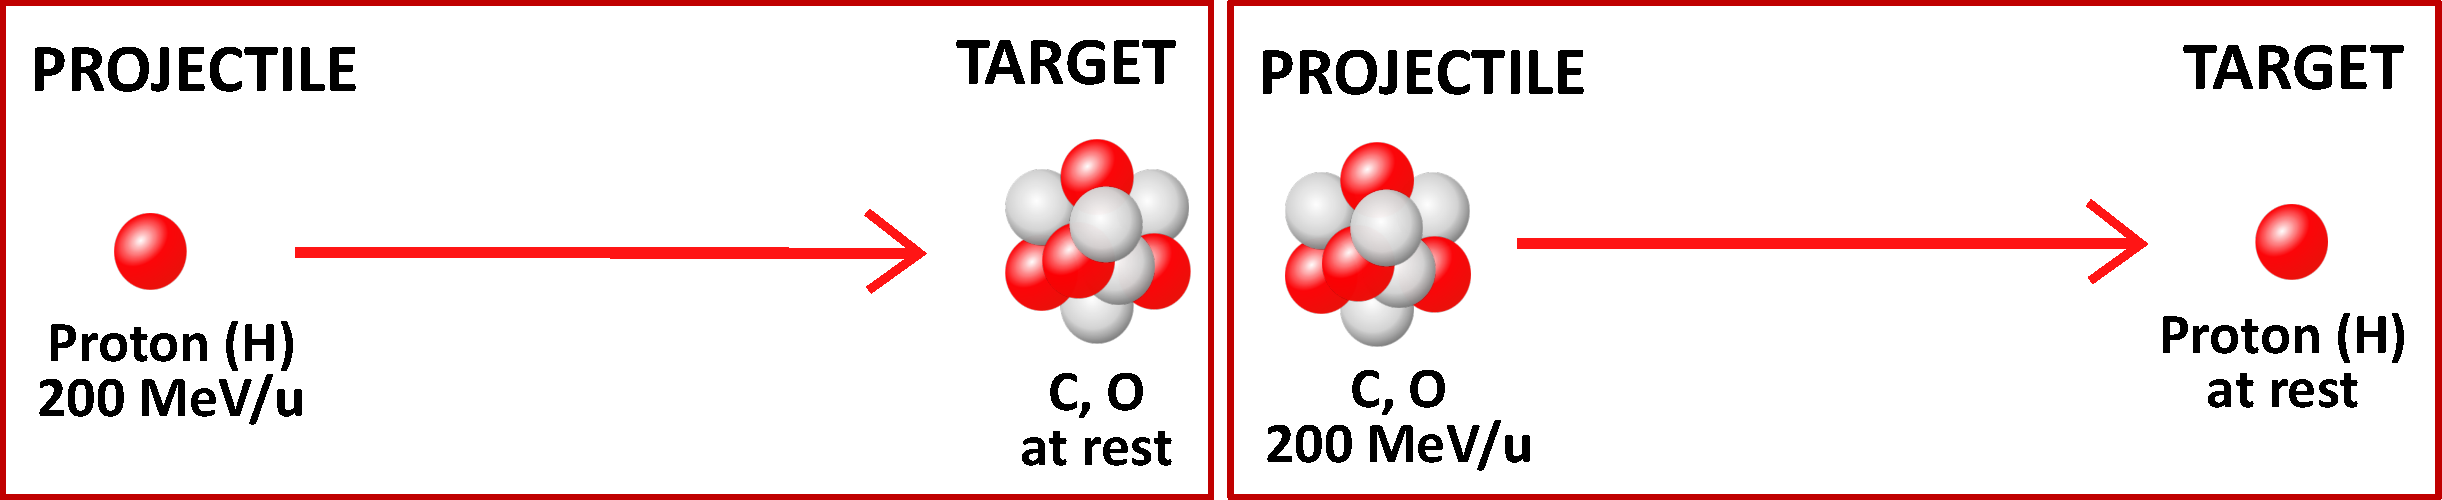
\includegraphics[width=0.98\linewidth]{inverse_kin.pdf}
	\caption[Direct and inverse kinematics]{On the left, a p-N reaction (direct kinematic), with the colliding nucleus at rest. On the right, a N-p reaction (inverse kinematic), with the colliding proton (\ce{H}) at rest.}
	\label{fig:inverse_kin}
\end{figure}
Actually, the inverse kinematic approach followed by the FOOT experiment is slightly more complicated than the one illustrated in \autoref{fig:inverse_kin}. Indeed, rather than using a fixed target composed of protons (\ce{H}), a fixed, hydrogen-enriched target is employed, still irradiated with \ce{^{4}He}, \ce{^{12}C} or \ce{^{16}O} beams. Solid hydrogenated materials (such as polyethylene, i.e., \ce{C2H4}) are preferred to pure hydrogen targets, primarily for technical reasons. Indeed, a dedicated liquid or gaseous hydrogen target requires extreme cryogenic conditions (around $T\simeq20\,\mathrm{K}$ for liquid \ce{H}) and cautious handling (due to \ce{H} flammability), both leading to potential safety and stability issues. Furthermore, liquid and gaseous \ce{H} need to be operated at pressures causing very low target densities, which result in inefficient measurements and, consequently, excessively long beam times with increased experimental costs \cite{17nq-3ddt}. Hence, to circumvent these technical difficulties, the hydrogen contribution to the N-p differential cross section is determined through a weighted subtraction method employing mono-atomic (e.g. graphite, \ce{C}) and composite targets (e.g. \ce{C2H4} or \ce{C5O2H8}). For example, \autoref{eq:c2h4} exploits complementary data acquired on \ce{C2H4} and \ce{C} targets:
\begin{equation}
	\begin{aligned}
		\left(\frac{d\sigma}{d\Omega}\right)_{\ce{H}}
		&=
		\frac{1}{4}
		\left[
		\left(\frac{d\sigma}{d\Omega}\right)_{\ce{C2H4}}
		-
		2\left(\frac{d\sigma}{d\Omega}\right)_{\ce{C}}
		\right],
		\\[0.5ex]
		\left(\frac{d\sigma}{dE_{\text{kin}}}\right)_{\ce{H}}
		&=
		\frac{1}{4}
		\left[
		\left(\frac{d\sigma}{dE_{\text{kin}}}\right)_{\ce{C2H4}}
		-
		2\left(\frac{d\sigma}{dE_{\text{kin}}}\right)_{\ce{C}}
		\right],
	\end{aligned}
	\label{eq:c2h4}
\end{equation}
where differential cross sections for producing a specific fragment $\text{k}$ with kinetic energy $E_{\text{kin}}$ and emission angle $\Omega$ are used. In \autoref{eq:c2h4}, the numbers $4$ and $2$ derive from the stoichiometric coefficients of \ce{C2H4}. The cross sections obtained from the difference method in \autoref{eq:c2h4} are compatible with the cross sections on pure hydrogen target, as shown by FLUKA simulations \cite{Ferrari:2005zk,BOHLEN2014211} presented in \cite{foot_cdr}, proving the validity of inverse kinematic.

Naturally, both PT and SRP applications require fragmentation cross section measurements for the original p-N interaction, therefore relativistic boost are eventually applied to \autoref{eq:c2h4}. These Lorentz transformations worsen the resolution on cross section measurements, not only because the kinematic quantities used to perform the boost (energy and momentum of the primary beam) have a limited precision, but also for the subtraction method itself. Indeed, the uncertainty propagation in \autoref{eq:c2h4} results in a quadratic sum of the errors obtained from each individual target measurement. That is the reason why reaching FOOT experimental goals on cross sections (see \autoref{sec:foot_aim}) demands high accuracy starting with the physical quantities of the primary ions (e.g., in-target impact point, incoming direction, energy and momentum) and of the emitted fragments (in-target production point, emission angle, energy and momentum).

Despite inevitably introducing additional uncertainties, the proposed inverse kinematic approach provides cross section measurements which would have been impossible otherwise \cite{measurement_impact_foot}. Another advantage of this method is that irradiating hydrogenated material with \ce{^{4}He}, \ce{^{12}C} or \ce{^{16}O} beams allows to study target fragmentation in parallel with projectile fragmentation, using respectively an inverse and a direct kinematic approach.
\section{Experimental setup}\label{sec:experimental_setup}
The FOOT experimental setup was carefully devised taking into account various radiobiological constraints, mainly driven by the physics of target and projectile fragmentation, and structural requirements. To address these requisites, extensive Monte Carlo simulations were implemented via the FLUKA software \cite{Ferrari:2005zk,BOHLEN2014211}, whose nuclear fragmentation models were deemed sufficiently robust to drive the design of FOOT apparatus. For example, in \autoref{fig:fluka_ekin_angle_dis} various FLUKA-simulated distributions of fragment emission angles and kinetic energies are shown. The prior experience of FIRST experiment at GSI \cite{PhysRevC.93.064601} was also of utmost importance to conceive the FOOT detector.
\begin{figure}[H]
	\centering
	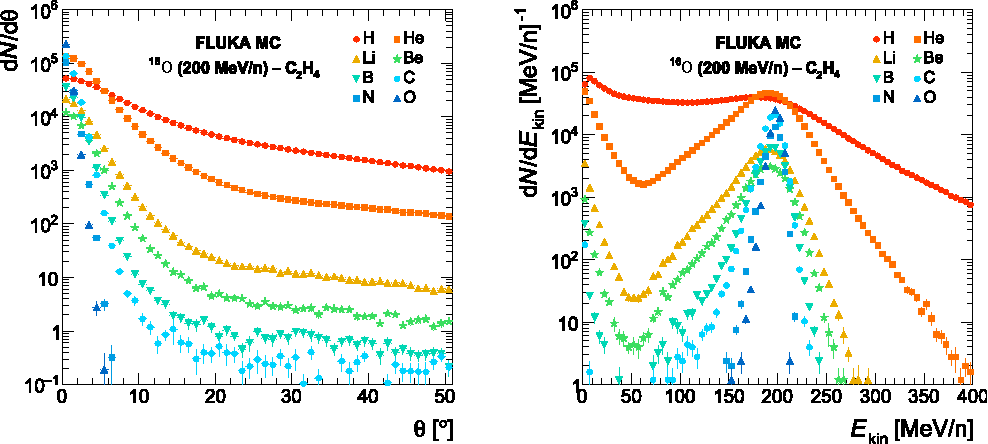
\includegraphics[width=0.98\linewidth]{group-MC7.pdf}
	\caption[Fragments' angular and kinetic energy distributions]{FLUKA Monte Carlo (MC) calculation of the angular (left) and kinetic energy (right) distributions of different fragments produced by a $200\,\mathrm{MeV/u}$ \ce{^{16}O} beam impinging on a \ce{C2H4} target \cite{measurement_impact_foot}.}
	\label{fig:fluka_ekin_angle_dis}
\end{figure}
The stringent requirements (see \autoref{sec:foot_aim}) on differential cross sections accuracy compel the FOOT experiment to perform charge and isotopic identification with a precision level of $2$--$3\%$ and $5\%$, respectively. In addition, the supplementary uncertainties introduced by inverse kinematic (see \autoref{sec:inv_dir_kin}) further constrain the uncertainties on fragment momentum and kinetic energy up to the few percent and demand a resolution of the mrad on the fragment emission angle with respect to the beam direction \cite{foot_cdr}. To limit the uncertainties even more, the FOOT apparatus is characterized by subdetector redundancies, which means that the same physical quantity is measured multiple times to reduce background noise and, accordingly, reconstruction artifacts (see \autoref{sec:electronic_setup}).

To measure nuclear fragmentation in the most efficient way, also the FOOT target needs to satisfy some essential requirements. First, its density should not be too large, otherwise in-target multiple coulomb scattering (see ?? MCS) would degrade the fragment angular resolution, spoiling the final differential cross section measurements. Second, a compromise on thickness should be met, as a very thick target produces an increased nuclear fragmentation statistic, while an excessive thickness leads to undesired energy losses within the target itself, which worsen the fragment energy measurement, and produces secondary fragmentation processes, which hinder the measurement of primary fragmentation cross sections. FLUKA simulation and experimental data show that the optimal areal density of the target material is $2$--$4\,\mathrm{g/cm^2}$, which sets a superior limit of $\simeq10^{-2}$ to the fragmentation probability \cite{measurement_impact_foot}.

While on the one hand the primary fragmentation probability needs to be maximized inside the target to increase relevant statistic, on the other out-of-target fragmentation must be minimized, as it falls outside the scope of FOOT. The main contributions to out-of-target fragmentation occur when particles break apart by colliding with air molecules, and when they fragment inside the support structures or the active parts of FOOT setup. These unwanted processes are relevant nor for PT neither for SRP physics, as they rather lead to potential reconstruction background that needs to be experimentally subtracted via software. To minimize fragmentation outside the target, FOOT apparatus has been specifically designed to possess a minimal material budget, where very-thin detectors are preferred to thicker ones. This design choice lowers out-of-target fragmentation as well as multiple coulomb scattering.

Two fundamental design choices of the FOOT detector are portability and compactness. The first allows to readily move the experimental setup to various therapeutic and research centers, including the National Center for Oncological Hadrontherapy (CNAO) in Pavia (Italy), the Heidelberg Ion Therapy Center (HIT) in Heidelberg (Germany) and the GSI in Darmstadt (Germany). The second facilitates the adaptability of FOOT apparatus into the research and experimental halls of beam facilities, which are often limited dimension-wise \cite{experimentalHallDim}. Detector transportability is not simply a sign of versatility, conversely, it is a core feature that will enable FOOT to study nuclear fragmentation from the diverse beam species and energies delivered by the aforementioned research facilities, in accordance with FOOT experimental program (detailed in \autoref{sec:foot_aim}).

The Monte Carlo plots shown in \autoref{fig:fluka_ekin_angle_dis}, corroborated by experimental data, predict that heavier fragments ($Z\geq3$) are forward peaked within a polar angle of $\simeq10^{\circ}$ with respect to the beam direction, and have kinetic energies centered around the $E_\text{kin}$ of the primary beam. Conversely, lighter fragments possess wider angular distributions and more variable kinetic energies. To maximize the angular acceptance and detection efficiency for both heavy and light fragments, the FOOT Collaboration has decided to divide the FOOT detector into two complementary experimental setups:
\begin{itemize}
	\item an electronic setup, with a magnetic spectrometer and tracking detectors, characterized by an angular acceptance of $\simeq10^{\circ}$ with respect to the beam direction. It is optimized to identify fragments heavier than \ce{^{4}He} ($Z\geq3$);
	\item an emulsion setup, with an emulsion spectrometer provided with , characterized by an angular acceptance up to $\simeq70^{\circ}$ in the polar angle, optimized to identify the isotopes of \ce{H} and \ce{He} ($Z\leq2$).
\end{itemize}
During data taking campaigns, each setup runs independently from the other and, for this reason, simultaneous data collection is not achievable. Despite longer beam time is required, each apparatus efficiently detects the fragments for which it was designed. In the following paragraphs, a detailed description of both setups will be provided, with particular emphasis on the electronic setup, which includes detectors analyzed more extensively in this work.
\section{Electronic setup}\label{sec:electronic_setup}
\begin{figure}[H]
	\centering
	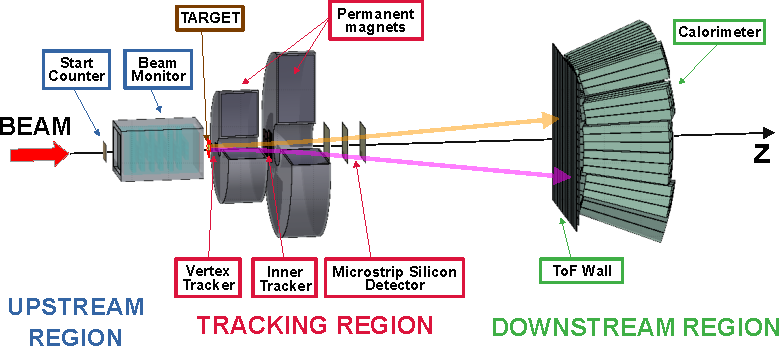
\includegraphics[width=0.98\linewidth]{electronic_setup.pdf}
	\caption[Electronic setup]{View of the electronic setup with its relevant detectors. In FOOT global frame of reference, the $z$ axis identifies the beam incoming direction. The production of $2$ fragments from beam-target interaction is also depicted. Revisited from \cite{Ubaldi_2025}.}
	\label{fig:electronic_setup}
\end{figure}
The FOOT electronic setup was designed to optimally detect fragments heavier than \ce{^{4}He} ($Z\geq3$), whose polar angles are contained within $\simeq10^{\circ}$ with respect to the beam direction. As sketched in \autoref{fig:electronic_setup}, the electronic setup is a $2$-$3\,\mathrm{m}$ long fixed-target detector comprising several subdetectors, employed to accurately measure fragment physical quantities such as Time of Flight (ToF), speed ($\beta=v/c$), momentum ($p$), kinetic energy ($E_\text{kin}$) and energy loss $\Delta E$. Combining these parameters, it is possible to uniquely identify the produced fragments by measuring their charge and mass reaching the maximum requested uncertainty of $2$--$3\%$ and $5\%$, respectively. To achieve such accuracy, high precision is necessarily required on the experimental quantities directly measured by FOOT. Both FLUKA Monte Carlo simulations and experimental data provide the following uncertainty ranges:
\begin{itemize}
	\item $\sigma(p)/p\simeq3$--$5\%$;
	\item $\sigma(\text{ToF})\simeq70$--$250\,\mathrm{ps}$;
	\item $\sigma(E_\text{kin})/E_\text{kin}\simeq1.5$--$2.5\%$;
	\item $\sigma(\Delta E)/\Delta E\simeq3$--$10\%$,
\end{itemize}
where the best performances refer to heavier fragments.
\begin{figure}[H]
	\centering
	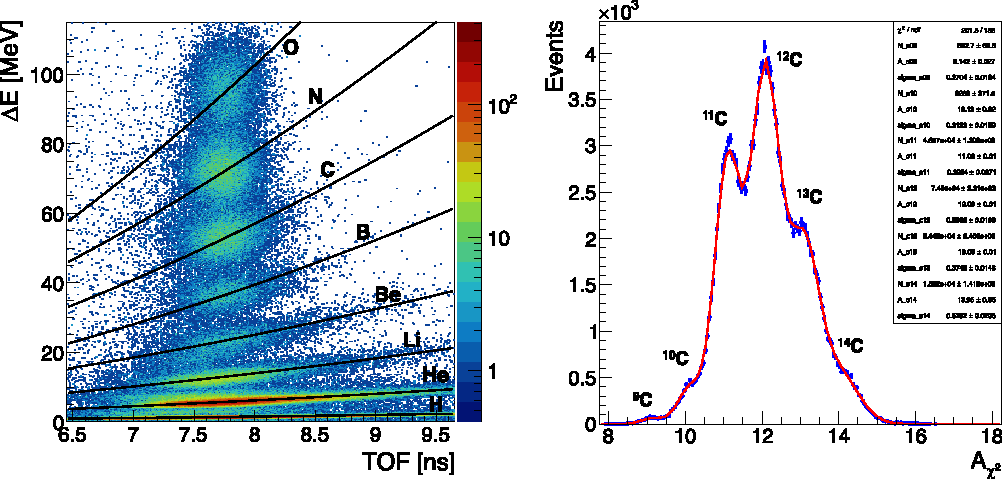
\includegraphics[width=0.98\linewidth]{charge_mass_id.pdf}
	\caption[Fragment charge and mass identification]{On the left, charge identification method (calibrated in \cite{KRAAN2021165206}) implemented using the energy release in the ToF Wall $\Delta E$ and the ToF calculation. For each cluster of points, a Bethe-Bloch curve (shown in black) is used to fit the Monte Carlo simulation data to describe the average energy loss of fragments with the same charge $Z$ impinging on the ToF Wall at different angles, kinetic energies, ToF and path lengths $L$. On the right, an example of mass number determination obtained with the $\chi^2$ fit for carbon fragments with $\sigma(ToF)\simeq70\,\mathrm{ps}$, $\sigma(p)/p\simeq3.7\%$ and $\sigma(E_\text{kin})/E_\text{kin}\simeq1.5\%$. Carbon isotopes are clearly visible. Extrapolated from \cite{measurement_impact_foot}.}
	\label{fig:charge_mass_id}
\end{figure}
As anticipated in \autoref{sec:experimental_setup}, detector redundancies contribute to reduce systematic uncertainties by estimating multiple times the same physical quantity. Specifically, the electronic setup employs redundancy to estimate particle charge and mass as a magnetic spectrometer:
\begin{itemize}
	\item charge identification is performed using the method in \autoref{fig:charge_mass_id} (left) by combining the ToF measurements with the $\Delta E$ deposited in a plastic scintillator named ToF Wall. In this method, the charge identification algorithm developed in \cite{10.3389/fphy.2022.979229} couples the measured $\Delta E$-ToF coordinate of a fragment to the closest Bethe-Bloch curve in \autoref{fig:charge_mass_id} (left). The charge $Z$ corresponding to the fitted Bethe-Bloch is eventually assigned to the fragment. This approach works because the Bethe-Bloch formula (see \autoref{eq:bethe_bloch}) depends on $\beta$, which in turn is a function of ToF:
	\begin{equation}
		\beta=\frac{v}{c}=\frac{L}{\text{ToF}\cdot c},
		\label{eq:beta}
	\end{equation}
	where $L$ is the path length traversed by the fragment. Redundancy in charge identification is achieved by independently measuring the energy $\Delta E$ released by fragments in the Microstrip Silicon Detector.
	\item The fragment mass is determined multiple times using the three relativistic expressions in \autoref{eq:relativistic_expr}, which combine two by two the momentum $p$, the kinetic energy $E_\text{kin}$ and the ToF (the latter is implicitly contained in the velocity $\beta$, as per \autoref{eq:beta}):
	\begin{equation}
		p=mc\beta\gamma,\quad
		E_\text{kin}=mc^2\left(\gamma-1\right),\quad
		E_\text{kin}=\sqrt{p^2c^2+m^2c^4}-mc^2,
		\label{eq:relativistic_expr}
	\end{equation}
	where $\gamma=1/\sqrt{1-\beta^2}$ is the Lorentz factor. From \autoref{eq:relativistic_expr}, the three mass estimate are:
	\begin{subequations}
		\begin{align}
			\label{eq:a1}
			A_1&=\frac{p}{u\beta c\gamma}\\
			\label{eq:a2}
			A_2&=\frac{E_{kin}}{uc^2\left(\gamma-1\right)}\\
			\label{eq:a3}
			A_3&=\frac{p^2c^2-E_{kin}^2}{2uc^2E_{kin}},
		\end{align}
	\end{subequations}
	where $u$ is the unified atomic mass unit ($\simeq931.5\,\mathrm{MeV}$). Despite being redundant, the \autoref{eq:a1}, \autoref{eq:a2} and \autoref{eq:a3} are not independent: by taking these formulae pairwise, they depend on physical quantities measured with the same subdetector. For example, both \autoref{eq:a1} and \autoref{eq:a3} depend on the momentum $p$ measurement. Even with the correlation on mass estimates, it is possible to take advantage of redundancy to attain the best mass estimation and its associated uncertainty. Specifically, the best mass estimate can be calculated algebraically either with a standard $\chi^2$ minimization or with an Augmented Lagrangian Method (ALM) \cite{Cho_2016}, whose results are compatible with each other. An example of the $\chi^2$ minimization technique is shown in \autoref{fig:charge_mass_id} (right), where the mass number determination of carbon isotopes is illustrated after a $\chi^2<5$ cut. A more detailed description of $\chi^2$ minimization and ALM procedures is respectively outlined in \autoref{ch:chi_squared_min} and \autoref{ch:alm_squared_min}.
\end{itemize}
The detectors constituting the electronic setup operate overall as a magnetic spectrometer, but they can be more precisely classified into three operating regions, as illustrated in \autoref{fig:electronic_setup}:
\begin{itemize}
	\item the upstream region (see \autoref{ssec:upstream_reg}), where the incoming beam firstly traverses a thin scintillating layer (Start Counter), which provides the initial trigger and the earliest ToF timestamp, and then passes through a drift chamber (Beam Monitor), which monitors the beam by measuring its direction and impact point after possible deviations occurred in the Start Counter. These measurements are fundamental to control the beam prior to its collision with the target, located at the end of the upstream region.
	\item The tracking region (see \autoref{ssec:tracking_reg}), which allows to determine the fragment trajectory and, from its curvature, the fragment momentum. A more detailed description of the reconstruction algorithm implemented to track nuclear fragments is specified in (?? global trk SHOE). The first detector of the tracking region is the Vertex Tracker, which measures the interaction point between the primary ion and the target. This vertex point corresponds to the fragment emission point. Successively, the produced fragments are bent by two permanent magnets, which are separated by two layers of silicon pixel (Inner Tracker) used for further tracking. After the magnetic region, the Microstrip Silicon Detector provides additional tracking points and measures the fragments' stopping power $dE/dx$ through $\Delta E$ deposition.
	\item The downstream region (see \autoref{ssec:downstream_reg}), located $\simeq1$--$2\,\mathrm{m}$ after the target (depending on the available space inside the experimental room), is used to measure the stopping power $dE/dx$ a second time from the $\Delta E$ released in the ToF Wall, which also provides the final ToF timestamp. At this level, the complete knowledge of ToF allows to compute the fragment $\beta$ via \autoref{eq:beta}. An electromagnetic Calorimeter closes the downstream region measuring the fragment kinetic energy $E_\text{kin}$.
\end{itemize}
More details on the functioning of FOOT electronic setup are described in the following sections.
\subsection{Upstream region}\label{ssec:upstream_reg}
The upstream region is composed of pre-target detectors which aim to monitor the beam by measuring its direction, the impact position inside the target and the number of impinging ions. This region is characterized by a minimal material budget to guarantee the least possible amount of interactions between the primary ions and the pre-target material. Hence, in the upstream section the minimal thickness traversed by the beam reduces both out-of-target fragmentation and multiple coulomb scattering.
\subsubsection{Start Counter}\label{sssec:start_counter}
The Start Counter (SC) is positioned at the very beginning of the electronic setup, approximately $20$--$30\,\mathrm{cm}$ before the target. It consists of a squared foil of EJ-228 plastic scintillator \cite{ej228datasheet} with a thickness of $250\,\mu\mathrm{m}$ and an active surface of $5\times5\,\mathrm{cm}^2$, sufficiently extended to cover the beam transverse size. As illustrated in \autoref{fig:start_counter}, the scintillator foil is supported by an aluminum frame enclosed in a black 3D printed box to ensure the adequate light tightness for detector operation, preventing the environmental light from generating scintillation light. When a primary particle interacts with the SC, the foil emits scintillation light, which is then collected laterally at each side (see \autoref{fig:start_counter}) by $12$ Hamamatsu $3\times3\,\mathrm{mm}^2$ SiPMs, each with a cell pitch of $25\,\mu\mathrm{cm}$ \cite{sipms_SC_datasheet}. forming a total of $48$ SiPMs. As shown in \autoref{fig:start_counter} (right), these $48$ SiPMs are bundled in eight electronic channels, each reading a group of $6$ SiPMs. The readout and powering of the SiPMs is handled by the WaveDAQ system \cite{GALLI2019399}, a custom trigger and data acquisition device able to sample signal rates up to $5\,\mathrm{GS/s}$ with a dynamic range of $1\,\mathrm{V}$. To amplify the incoming signal before digitization, the WaveDAQ provides a modifiable gain between $0.5$ and $100$ that maximizes the detector efficiency based on the beam energy and composition. This amplification compensates the low light yield generated by the very thin SC scintillator foil. Once the digitized waveforms are generated, they are analyzed offline through a constant fraction discriminator technique to extrapolate the event timestamp independently of the incoming signal amplitude \cite{Wiebusch_2024}.
\begin{figure}[H]
	\centering
	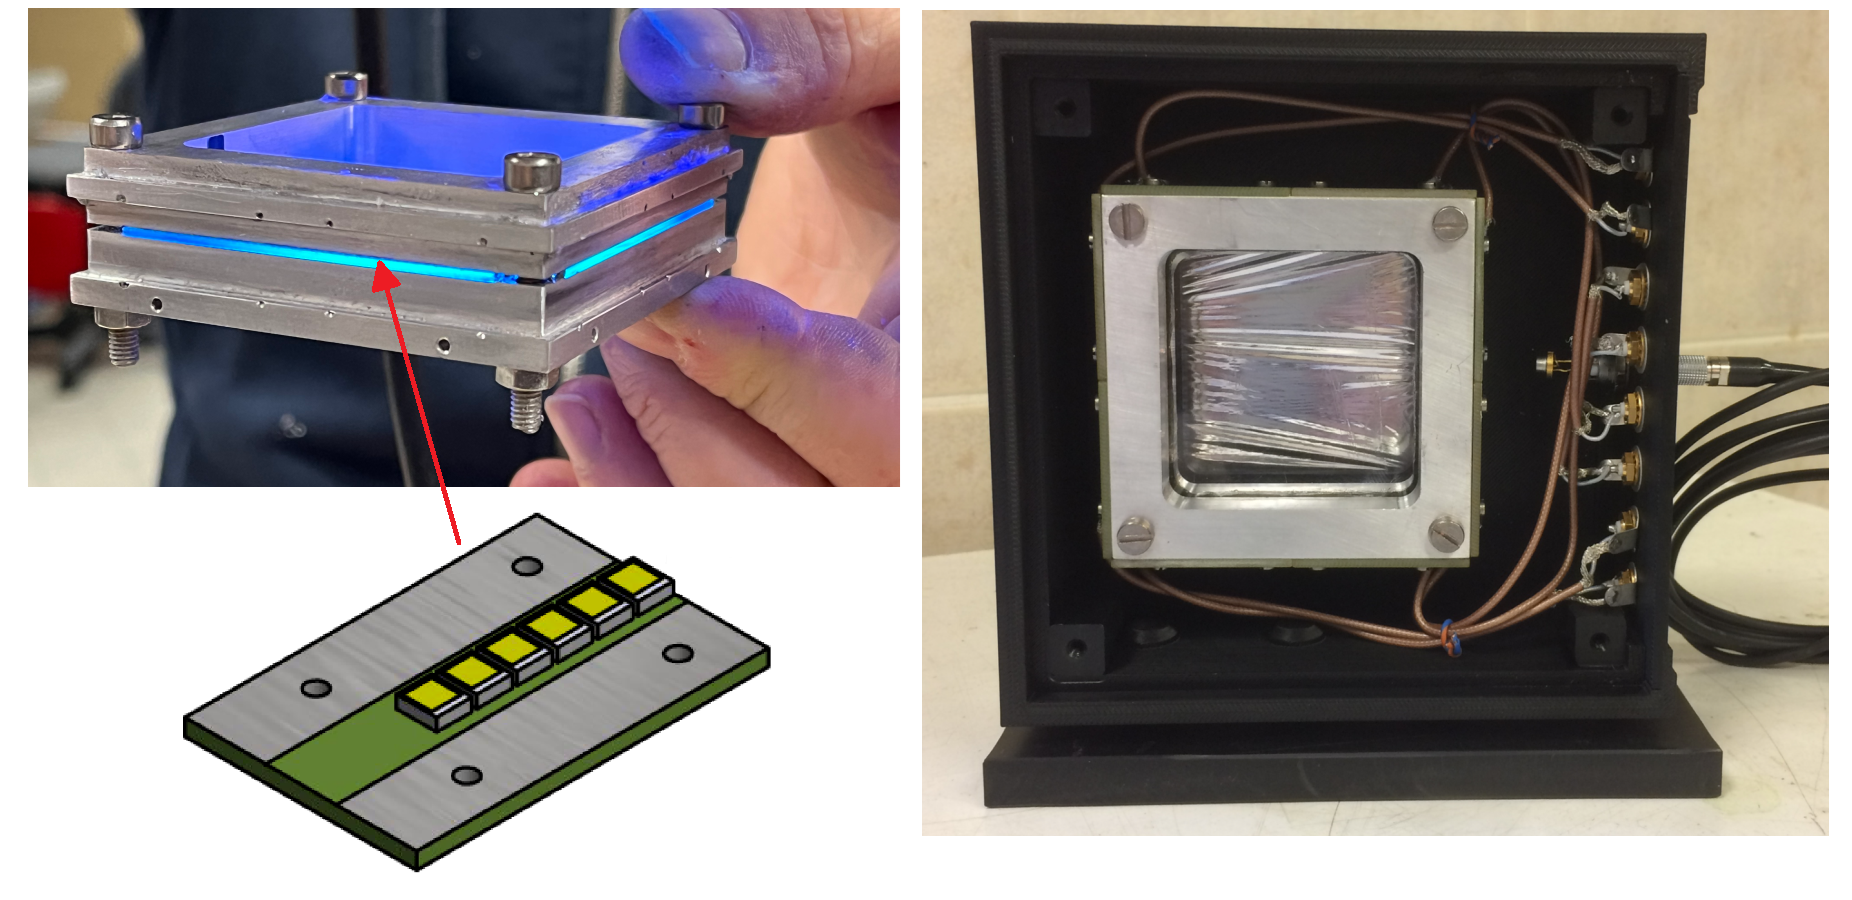
\includegraphics[width=0.98\linewidth]{start_counter.png}
	\caption[Start Counter]{SC plastic scintillator inside its aluminum frame (top left), surrounded by the outer black casing (right) to shield it from the environmental background light. A group of lateral SiPMs is also sketched (bottom left). Adapted from \cite{UbaldiPhDThesis,Traini2019FOOT}.}
	\label{fig:start_counter}
\end{figure}
The tasks fulfilled by the SC include measuring the initial timestamp of the ToF (whose final timestamp is provided by the ToF Wall, see \autoref{sssec:tof_wall}), distributing the reference time of a FOOT event\footnote{An event in FOOT represents the sequence of events where a single beam particle firstly interacts with the SC, then collides with the target and finally produces (or not) nuclear fragments.} to all the other detectors, generating the minimum bias trigger (see \autoref{ssec:tdaq_electronic_setup}) and evaluating the beam ion flux. To guarantee the rapid synchronization of the whole electronic setup, the SC possesses a precise time resolution of $50\,\mathrm{ps}$ (according to the CNAO 2024 campaign with $400\,\mathrm{MeV/u}$ \ce{^{12}C} ions \cite{UbaldiPhDThesis}) and an efficiency for primaries' detection close to $1$ at rates $\lesssim10\,\mathrm{kHz}$ (as reported in \cite{Haidar_2012}).
\subsubsection{Beam Monitor}\label{sssec:beam_monitor}
Following the beam direction, after the SC the primary ions cross the Beam Monitor (BM), a drift chamber filled with a gaseous mixture of $\ce{Ar}/\ce{CO2}$ at $80/20\%$, respectively, kept approximately at ambient pressure ($\simeq0.9\,\mathrm{bar}$). As illustrated in the technical drawing in \autoref{fig:beam_monitor} (left), the BM drift chamber is composed of $12$ groups of wire layers oriented orthogonally with respect to the beam direction, which reconstruct the beam position in both the $x$ and $y$ coordinates. The horizontal and vertical layers, independently, are staggered by half a cell to solve left-right hit ambiguities in track reconstruction, as sketched in \autoref{fig:beam_monitor2}. Additionally, as presented in \autoref{fig:beam_monitor2}, each wire layer consists of $3$ rectangular drift cells with dimension $16\times10\,\mathrm{mm}^2$. The organized network of wires (see \autoref{fig:beam_monitor} (right)) allows the BM to achieve a $\simeq90\%$ detection efficiency for a wide range of beams and energies \cite{RidolfiPhDThesis}, a good spatial resolution of $100\,\mu\mathrm{m}$ towards the BM center and an angular resolution of $2\,\mathrm{mrad}$ \cite{DONG2021164756}.
\begin{figure}[H]
	\centering
	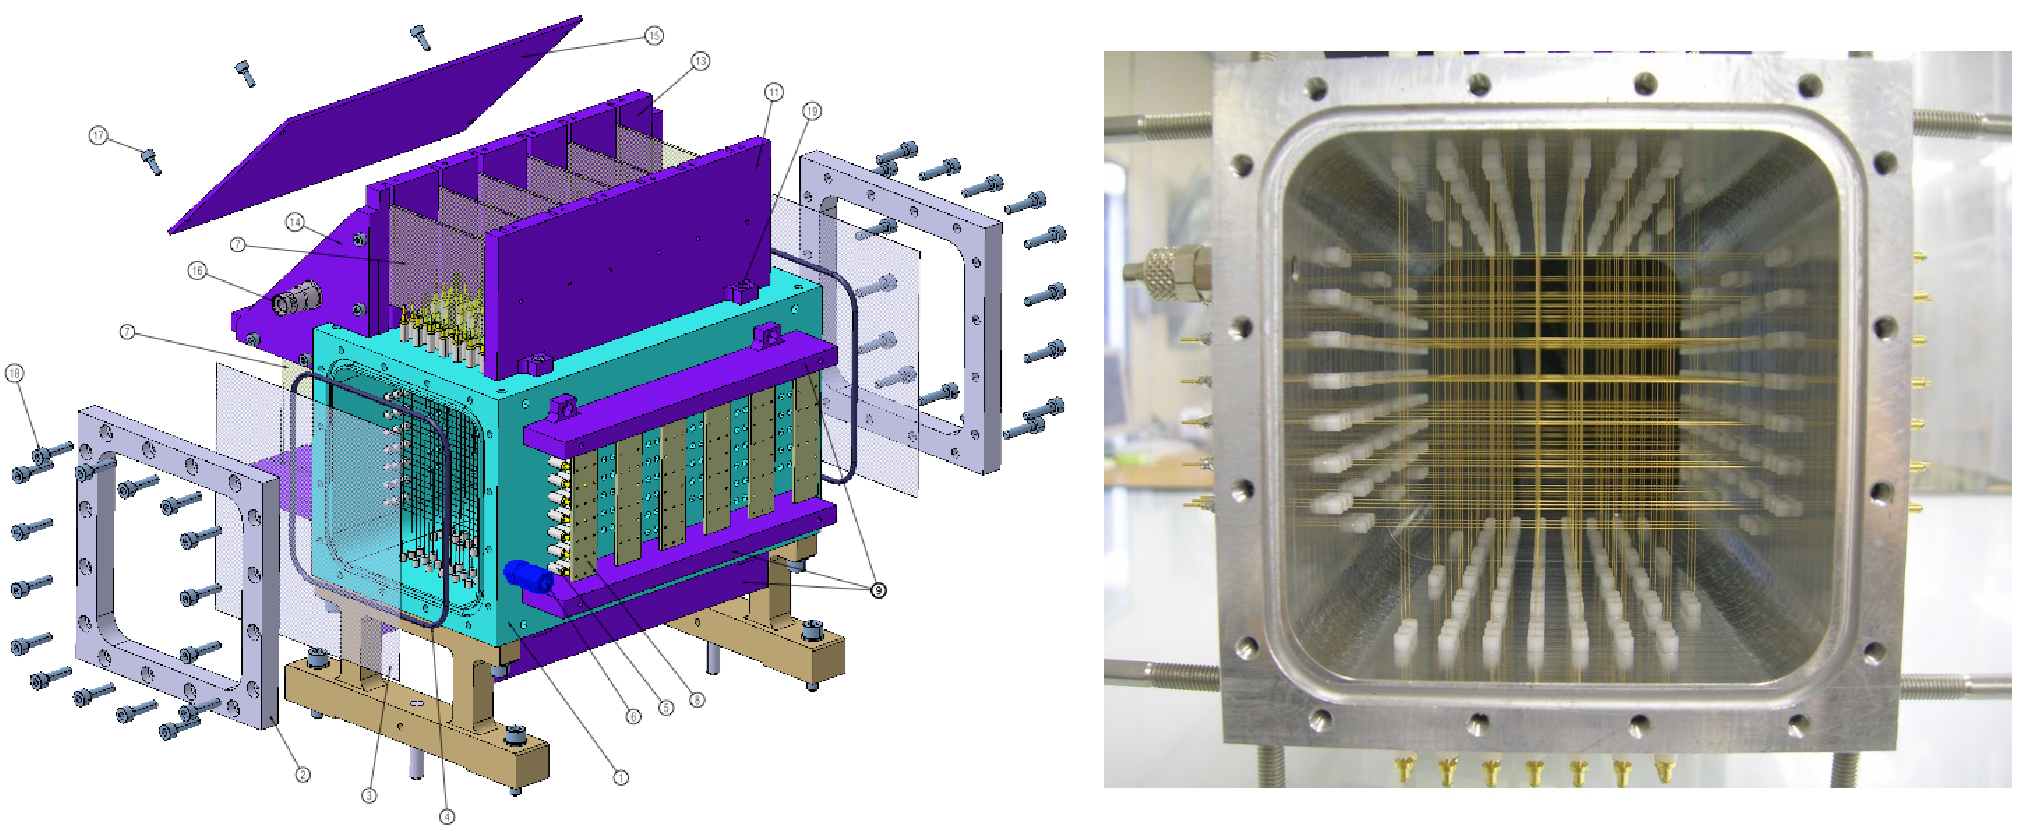
\includegraphics[width=0.98\linewidth]{beam_monitor.png}
	\caption[Beam Monitor]{On the left, a technical drawing of the BM. On the right, a more detailed view of the inner drift chamber is shown. Adapted from \cite{measurement_impact_foot}.}
	\label{fig:beam_monitor}
\end{figure}
Being located between the SC and the target, the BM accomplishes the crucial task of measuring the beam direction and impact position on the target after possible deflections occurred in the SC. Moreover, the gas rarefaction of the BM offers the paramount advantage of not further deviating the primary ions, ensuring precise beam position measurements without inducing additional systematic effects. The accurate spatial information provided by the BM allows to understand whether deflected tracks had previously generated fragmentation inside the SC. Thus, the BM can be also employed as a veto tool to reduce out-of-target fragmentation, as well as the pile-up ambiguities in the tracking devices beyond the target. Pile-up happens when more than one primary particle or multiple fragmentation processes are registered in the same event, representing a major concern for the analysis software performing the offline event reconstruction. This pile-up removal can be efficiently performed only if the BM is precisely aligned to the detectors located after the target.

The high spatial and angular resolutions of the BM are particularly relevant for the inverse kinematic approach (see \autoref{sec:inv_dir_kin}). Indeed, the $100\,\mu\mathrm{m}$ and $2\,\mathrm{mrad}$ resolutions allow to correctly determine the fragment emission angle with respect to the beam direction, of utmost importance for the Lorentz boost needed for the inverse kinematics.
\begin{figure}[H]
	\centering
	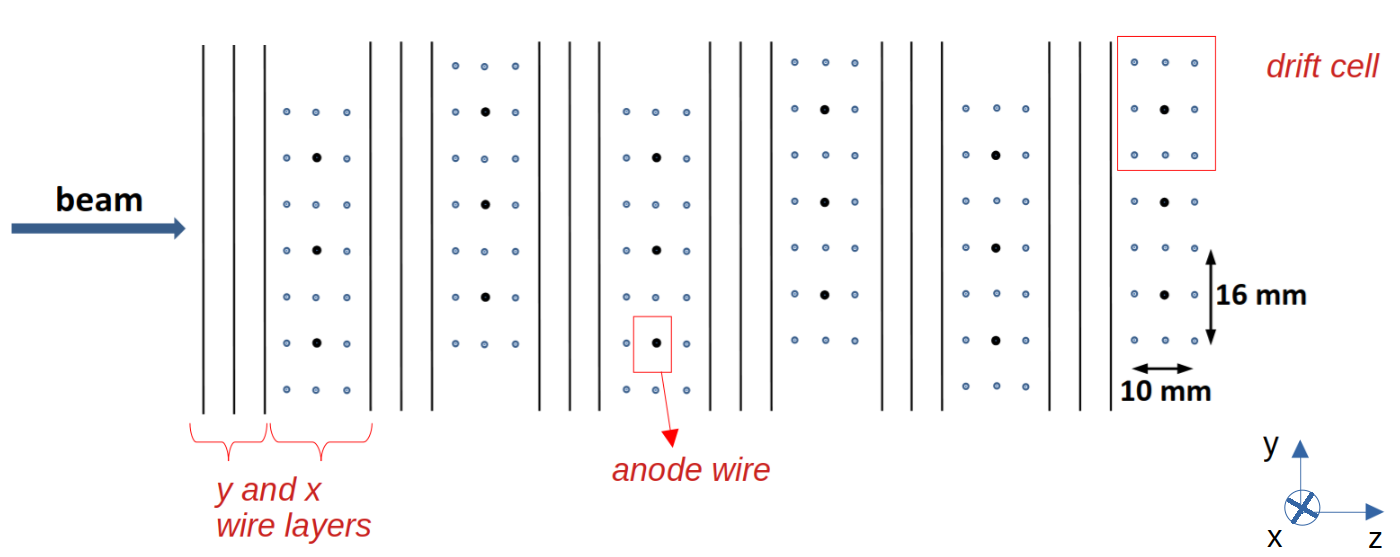
\includegraphics[width=0.98\linewidth]{beam_monitor2.png}
	\caption[Beam Monitor wire scheme]{Detailed structure of BM drift chamber, adapted from \cite{UbaldiPhDThesis}.}
	\label{fig:beam_monitor2}
\end{figure}
\subsection{Tracking region}\label{ssec:tracking_reg}
The tracking region represents the operating core of the electronic setup, which effectively acts as a magnetic spectrometer. In \autoref{fig:tracking_region} (left) the concept of the tracking region is illustrated: three silicon measuring stations are located before, between and after two permanent magnets. With a magnetic field oriented towards the $y$ direction (see \autoref{fig:tracking_region} (right)), the two permanent magnets bend trajectories to evaluate the fragment rigidity $p/Z$, from which the momentum $p$ can be derived. As detailed in (?? sec global analysis), fragment trajectories are reconstructed via a GENFIT-based \cite{Rauch_2015} reconstruction algorithm named SHOE (Software for Hadrontherapy Optimization Experiment) developed by the FOOT Collaboration. To minimize fragmentation inside the silicon sensors and multiple coulomb scattering, detector thinness was a design priority. For this reason, the monolithic pixel technology was chosen in the first two stations, while for the last one thin strips were preferred.
\begin{figure}[H]
	\centering
	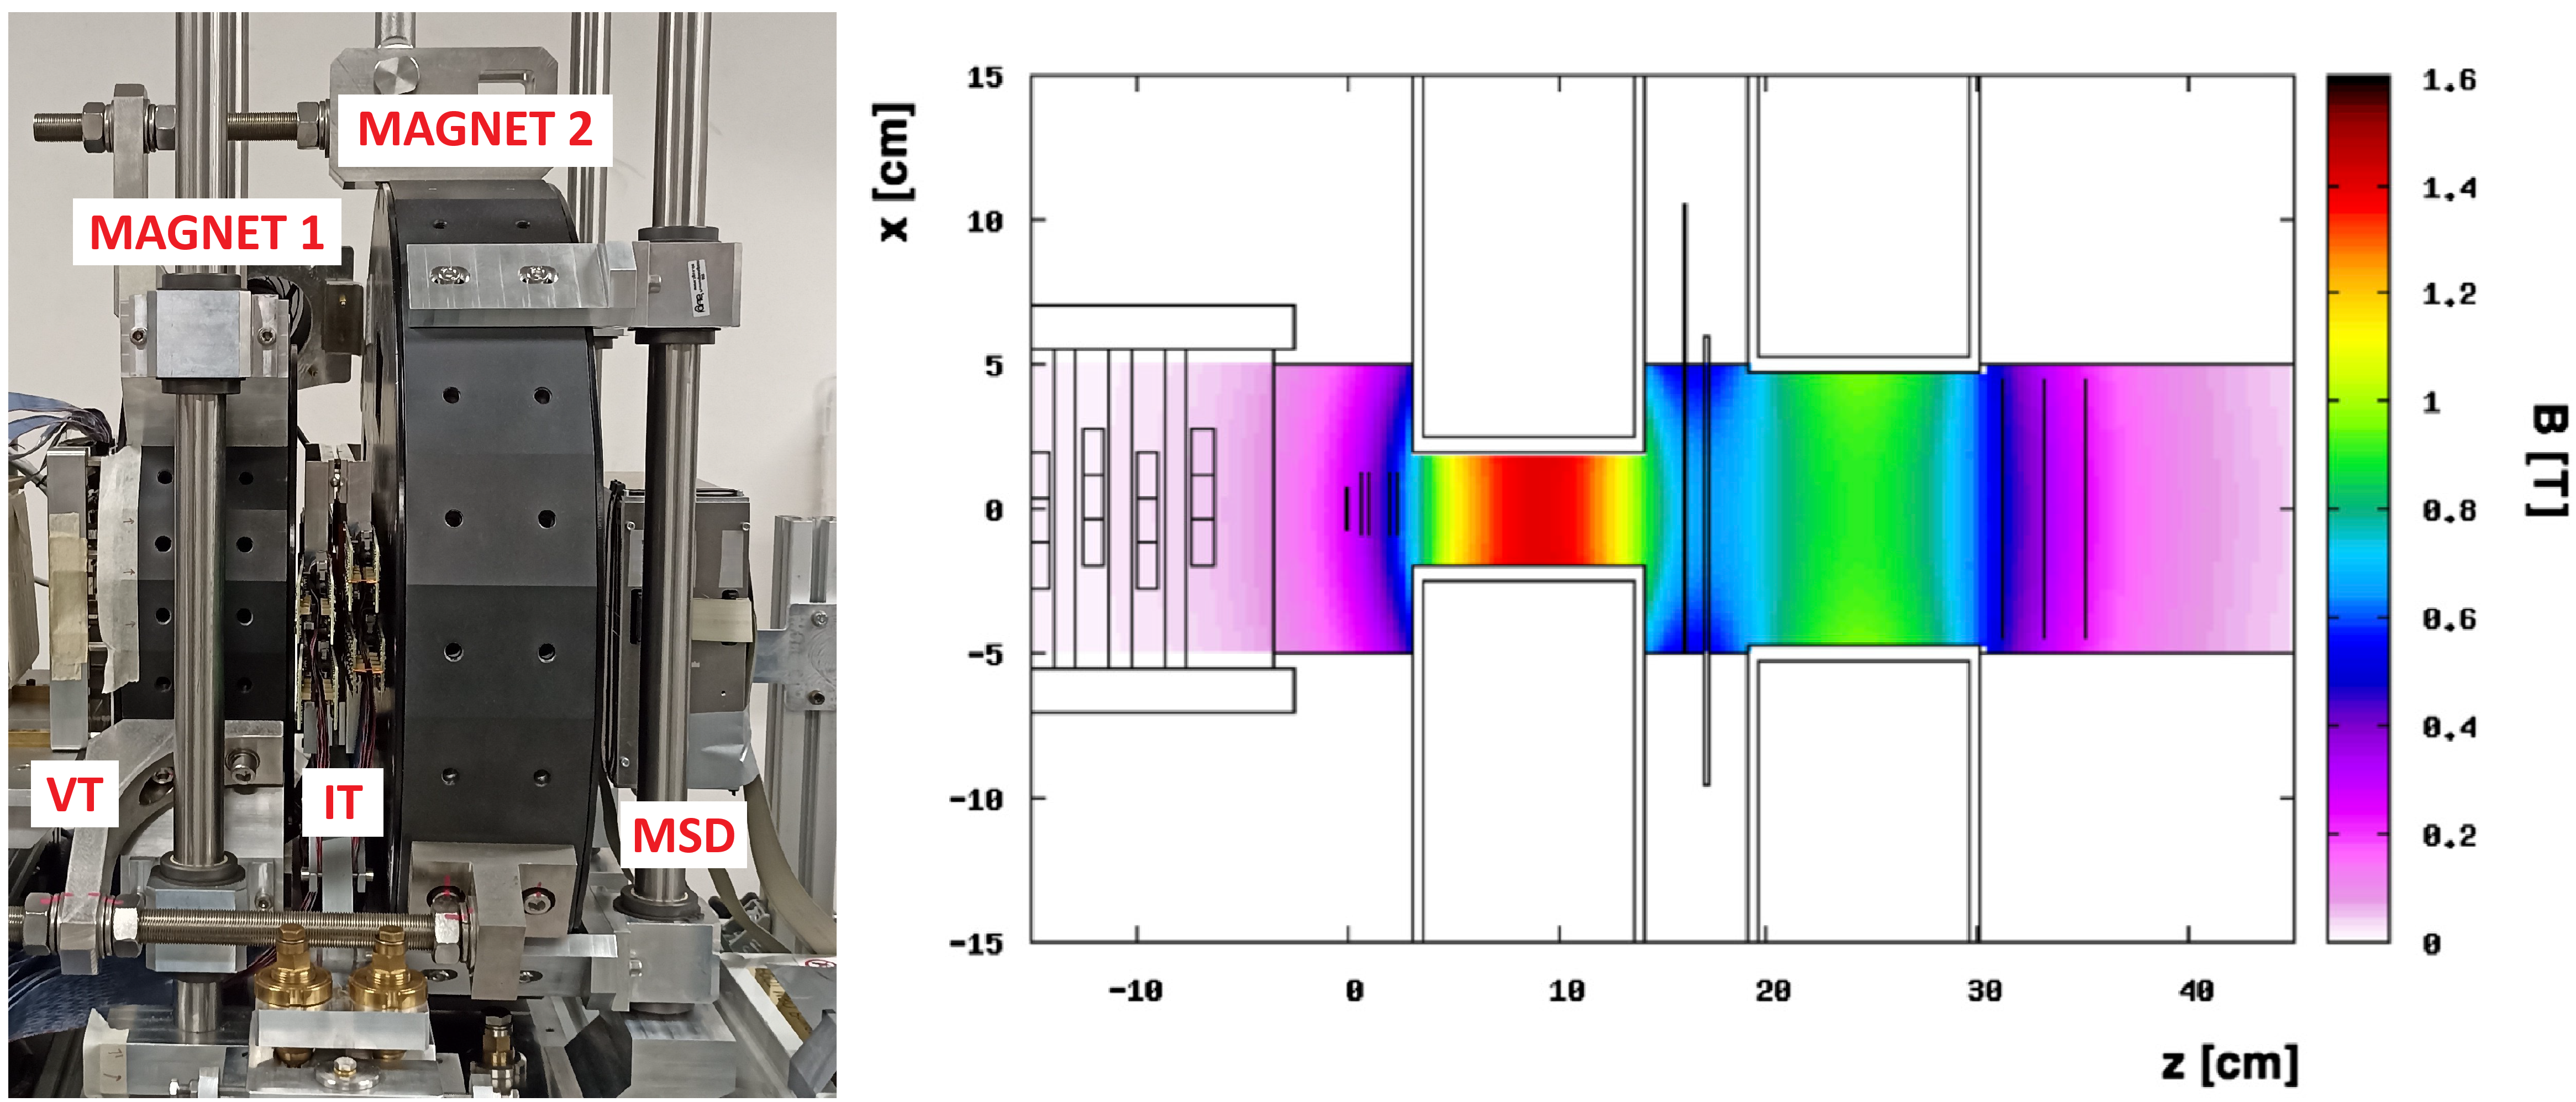
\includegraphics[width=0.98\linewidth]{tracking_region.png}
	\caption[Tracking region]{On the left, picture of the FOOT magnetic spectrometer during a CNAO data taking campaign. In FOOT global frame of reference, the $y$ axis runs vertically, while the $z$ axis runs horizontally. The beam comes from the left, along the $z$ axis, crosses sequentially the target (not shown), the Vertex Tracker (VT), the magnets and the Inner Tracker (IT) and, finally, the Microstrip Silicon Detector (MSD). All the detectors are found inside the mechanical framing shown in the picture. On the right, computed magnetic field map generated by FOOT magnets in Halbach configuration. The magnetic field intensity $B(T)$, shown in the lateral palette, is referred to its $y$ axis component. Adapted from \cite{measurement_impact_foot,ZarrellaPhDThesis}.}
	\label{fig:tracking_region}
\end{figure}
\subsubsection{Vertex Tracker}\label{sssec:vertex_tracker}
Being situated just $\lesssim1\,\mathrm{cm}$ after the target, the Vertex Tracker (VT) is undoubtedly the most relevant tracking station of the electronic setup. Indeed, the VT is essential not only to reconstruct the initial fragment path, but also to find the interaction point between the primary ion and the target, which determines the fragment emission point (hereinafter also denominated VT point). As shown in \autoref{fig:vertex_tracker} (left), the VT consists of $4$ detection layers situated along the $z$ axis, each with an active area of $\simeq2\times2\,\mathrm{cm}^2$, providing a total angular acceptance of $\simeq40\,^{\circ}$.\footnote{Such angular acceptance cannot be fully exploited due to the overall electronic setup's angular acceptance of $\simeq10\,^{\circ}$.}

To minimize the VT thickness, each detection layer adopts the MIMOSA-28\footnote{MIMOSA stands for Minimum Ionizing MOS Active pixel sensor.} (M28, see \autoref{fig:vertex_tracker} (right)) CMOS Monolithic Active Pixel Sensors (MAPS) technology, particularly suitable in low material budget applications due to the fact that both the sensor and the readout electronics are integrated onto the same silicon wafer, guaranteeing a layer thickness of just $50\,\mu\mathrm{m}$, resulting in a total thickness of $200\,\mu\mathrm{m}$ for the entire VT. The M28 sensor, originally built for the STAR experiment at RHIC \cite{GREINER201168,Valin_2012} and later employed in PT and SRP applications \cite{REIDEL2021165807}, is constituted by a matrix of $928\,\mathrm{rows}\times960\,\mathrm{columns}$ pixels with a pitch of $20.7\,\mu\mathrm{m}$, which allows for a spatial resolution of $\simeq5\,\mu\mathrm{m}$ after performing an appropriate alignment procedure \cite{REIDEL2019142,SPIRITI201735}. The VT high spatial resolution is able to resolve the $\mathrm{mrad}$ when measuring the fragment emission angles. This, combined with the precise evaluation of the beam direction at the $\mathrm{mrad}$ level provided by the BM (see \autoref{sssec:beam_monitor}), is beneficial to the relativistic transformations applied to the inverse kinematic method (see \autoref{sec:inv_dir_kin}).
\begin{figure}[H]
	\centering
	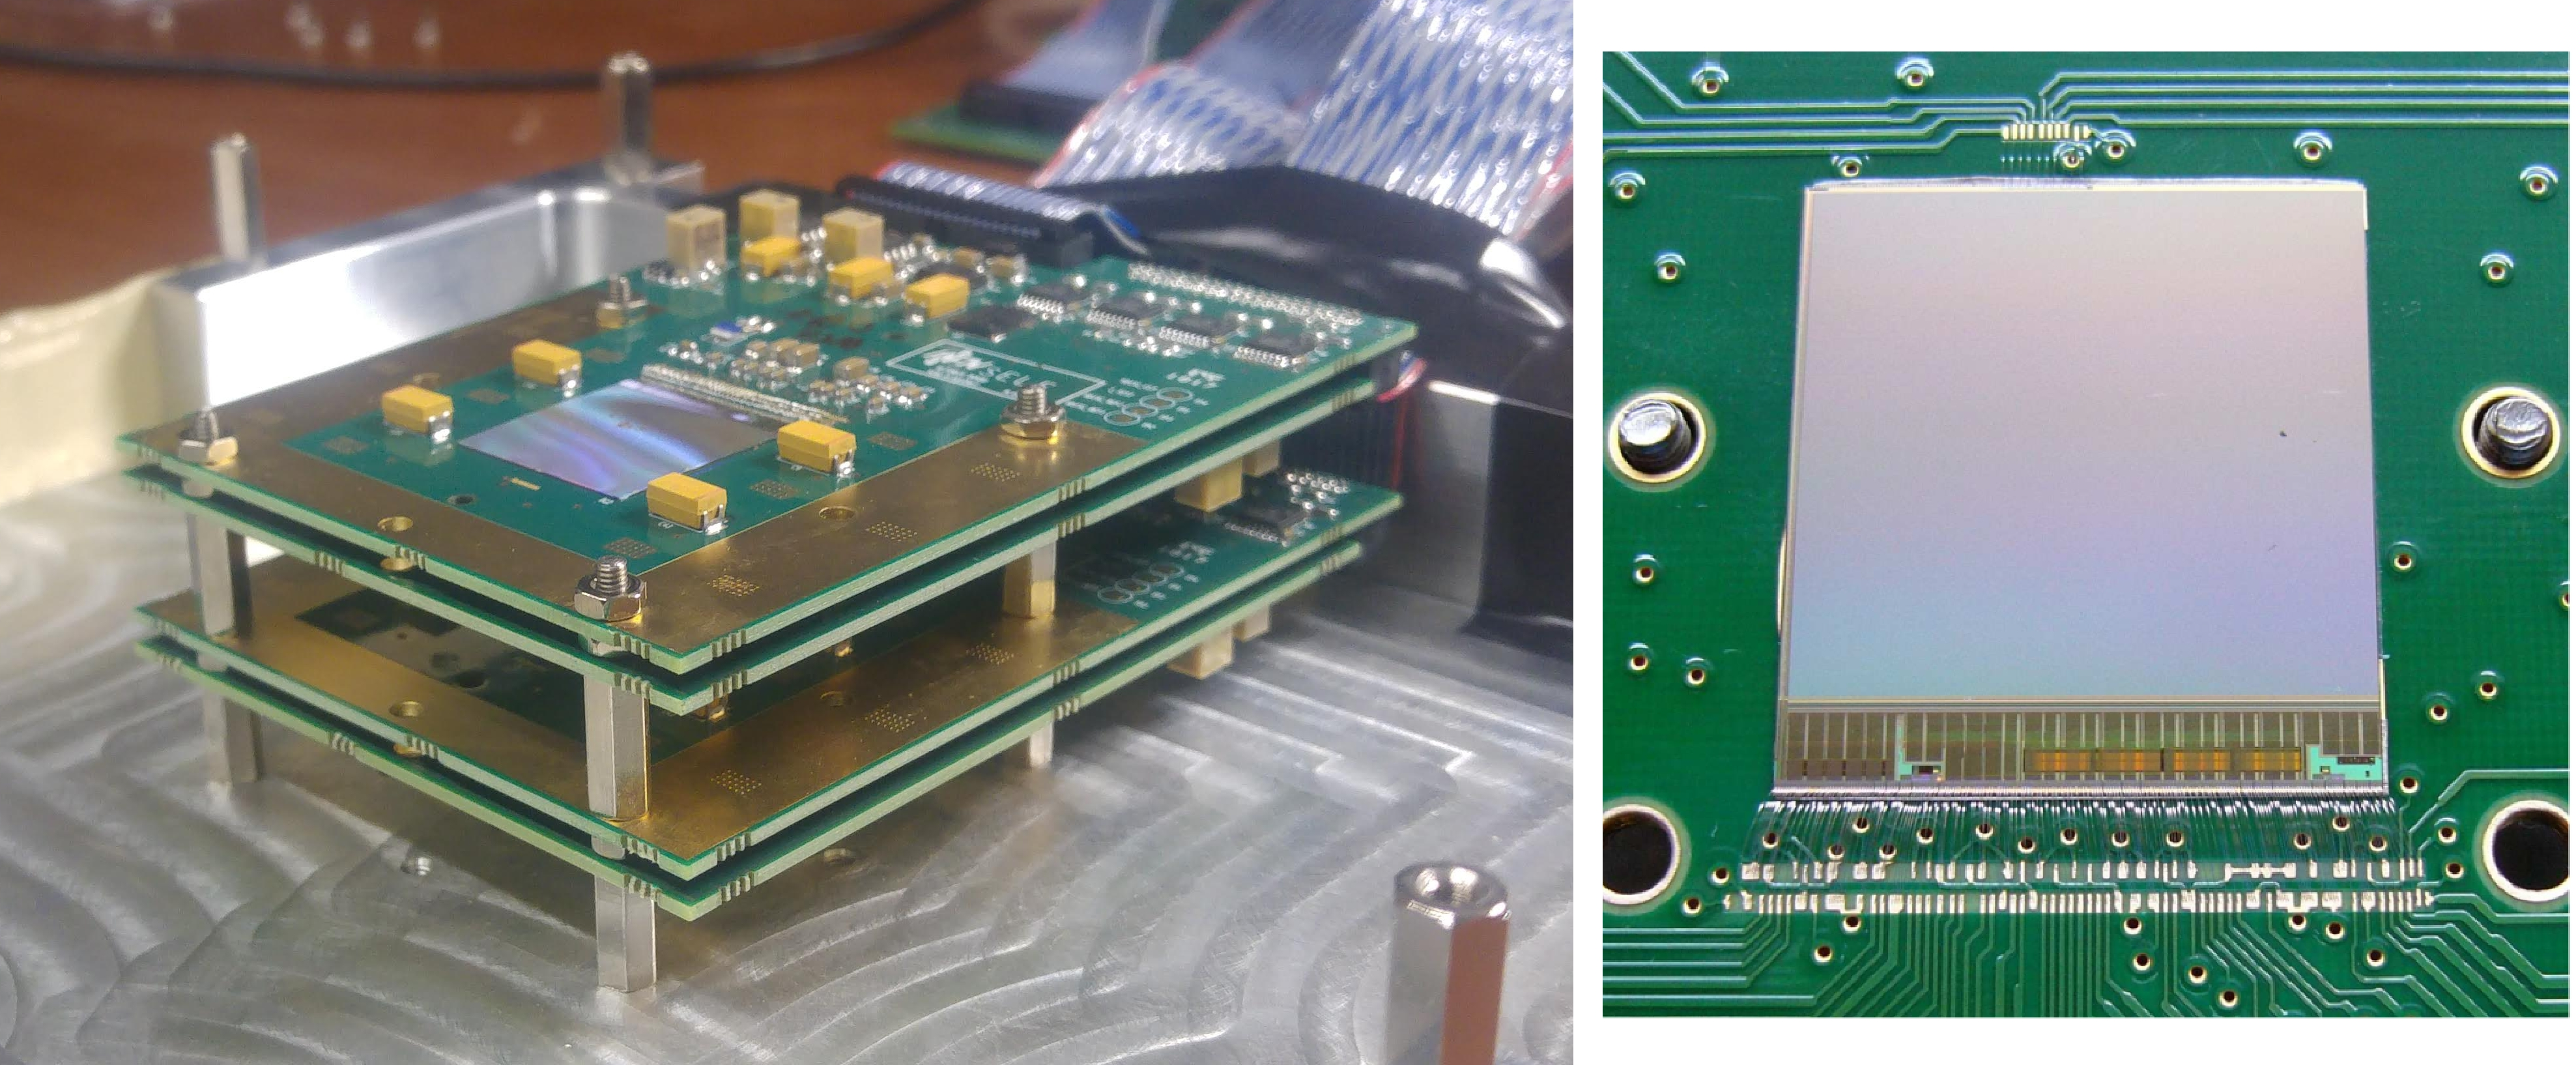
\includegraphics[width=0.98\linewidth]{vertex_tracker_jpg.jpg}
	\caption[Vertex Tracker]{Pictures of the $4$ detection planes of the VT (left) and of MIMOSA-28 chip (right) \cite{UbaldiPhDThesis,ZarrellaPhDThesis}.}
	\label{fig:vertex_tracker}
\end{figure}
The MIMOSA-28 technology in \autoref{fig:vertex_tracker} (right) can be further examined at the pixel level considering \autoref{fig:maps}, which schematized a CMOS MAPS. Monolithic CMOS are composed of a moderately p-doped thin epitaxial layer (P$-$) delimited by two highly p-doped regions, the substrate (P$++$) and the P-well (P$++$). At the top of each pixel, a N-well (N$++$) implant immersed in the superior P-well creates a pn junction at the P$-$/N$++$ boundary, that corresponds to the collection diode. When a charged particle traverses the epitaxial layer, electron-hole pairs are produced by ionization. Due to diffusion gradients and electric field drifts, electrons move towards the N-well implant inducing a signal, which is then stored in a diode-parasitic capacitance \cite{Reidel03177291}. Subsequently, each pixel amplifies the induced analog signal adopting the readout electronics embedded in the P- and N- wells (not explicitly shown in \autoref{fig:maps}).
\begin{figure}[H]
	\centering
	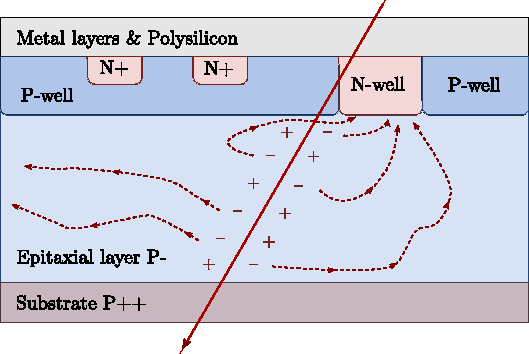
\includegraphics[width=0.8\linewidth]{maps.pdf}
	\caption[Monolithic Active Pixel Sensor scheme]{Schematic drawing of a MAPS devoted to charged particle detection. The particle trail (red solid line) ionizes the epitaxial layer to induce electron drift and diffusion processes (red dotted lines) towards the N-well diode. From \cite{Reidel03177291}.}
	\label{fig:maps}
\end{figure}
Contrary to fully depleted CMOS sensors, the MAPSs of M28 are only partly depleted \cite{UbaldiPhDThesis}. Consequently, the movement of the generated electron-hole pairs is primarily influenced by the diffusion component rather than the drift, which instead becomes predominant only in the vicinity of the pn junction where more intense built-in voltages are induced. The stronger diffusion contribution may lead to wider diffusion clouds that may cause electrons to move over adjacent pixels, leading to the formation of clusters. The cluster size, i.e., the number of pixels fired by the passage of a single particle, is correlated with the charge $Z$ of the traversing fragment: particle with higher atomic number $Z$ deposit more energy according to \autoref{eq:bethe_bloch} producing more ionization, consequently generating larger cluster sizes. Hence, in addition to the charge identification performed by the Microstrip Silicon Detector (see \autoref{sssec:microstrip_silicon_detector}) and the ToF Wall (see \autoref{sssec:tof_wall}), the cluster size of the VT provides support for measuring the fragment charge \cite{REIDEL2021165807}.

Despite the partial depletion of M28 pixels, their epitaxial layer has a resistivity of $400\,\Omega\cdot\mathrm{cm}$, which exceeds the standard $10\,\Omega\cdot\mathrm{cm}$ of the previous MIMOSA-26 device, ensuring enhanced signal-to-noise ratio and superior radiation tolerance. Each M28 pixel integrates a binary readout (hit/no hit) with an in-chip zero suppression mechanism to reduce the data transfer load off-chip. Moreover, it includes a Correlated Double Sampling (CDS) circuitry, which removes undesired offsets. The M28 $\simeq1$ million pixels are readout via a rolling shutter technique, which employs $960$ end-of-column discriminators to readout columns in parallel and produce a digitized binary information for each pixel. The readout time takes $185.6\,\mu\mathrm{s}$, allowing a frame rate of $\simeq5\,\mathrm{kHz}$.

The VT readout is implemented with a Terasic DE10 board system housing an Intel/Altera System-on-Chip (SoC) FPGA (Cyclon V) with a dual-core Cortex-A9 CPU. The FPGA interfaces the VT sensors with the Trigger and Data Acquisition control, which handles trigger, time-stamping and busy signals. Once a triggering event occurs, the CPU is finally employed to send data to the central DAQ via a $1\,\mathrm{Gb}$ Ethernet connection \cite{measurement_impact_foot}.
\subsubsection{Inner Tracker}\label{sssec:inner_tracker}
\begin{figure}[H]
	\centering
	\includegraphics[width=0.6\linewidth]{inner_tracker2.png}
	\caption[Inner Tracker]{At the top, technical drawing of the $4$ ladders hosting $8$ back-to-back sensors each for the IT. At the bottom, a front view of the $4$ M28 chips attached together to form one side of the ladder. From \cite{UbaldiPhDThesis}.}
	\label{fig:inner_tracker}
\end{figure}
To achieve the required momentum resolution, an additional tracker named Inner Tracker (IT) is located in the cavity between the two permanent magnets, as illustrated in \autoref{fig:tracking_region} (left). The IT measures the particle trajectory after the deflection provided by the first magnet. To simplify the DAQ architecture, the IT was developed using the same M28 MAPS technology of the VT (see \autoref{sssec:vertex_tracker}), with the mere difference that only $2$ detecting planes (with larger extension) are foreseen, each composed of $16$ M28 sensors covering a total sensitive area of $8\times8\,\mathrm{cm}^2$ per layer. The IT tracking performances are not influenced by the residual $\simeq0.6\,\mathrm{T}$ magnetic field in the gap between the permanent magnets \cite{DEBOER2002163}, where the IT is positioned.

As schematized in \autoref{fig:inner_tracker} (top), the IT was built using groups of ladders, a method similarly explored in the PLUME project \cite{SMeroli_2011}. Each of the $2$ staggered IT layers possesses two ladders orthogonal with respect to the beam direction and separated in the vertical $y$ axis by $\simeq1\,\mathrm{cm}$. Every ladder hosts $8$ M28 sensors arranged on both sides, with a back-to-back spacing of $2\,\mathrm{mm}$. Hence, in each side of the ladder, $4$ glued M28 sensors are attached together, as shown in \autoref{fig:inner_tracker} (bottom).
\subsubsection{Permanent magnets}\label{sssec:permanent_magnets}
To perform the momentum measurement, fragment trajectories are bent by $2$ permanent magnets, represented in \autoref{fig:tracking_region} (left). To meet the requirements on momentum resolution (see \autoref{sec:electronic_setup}) and on the portability of the apparatus, two hollowed magnets in Halbach configuration were chosen, both composed of multiple blocks made of Neodymium-Iron-Boron material (see \autoref{fig:permanent_magnets}). The Halbach configuration guarantees an approximately constant magnetic field $B(T)$ inside the internal cylindrical hole and a negligible $B(T)$ outside the cylinders, as illustrated in the field map of \autoref{fig:tracking_region} (right). The precise mapping of magnetic field lines is essential to track fragments, as reconstruction algorithms employ numerical methods to track charged particles and, consequently, measure their momentum (further details are provided in ?? sec global analysis).
\begin{figure}[H]
	\centering
	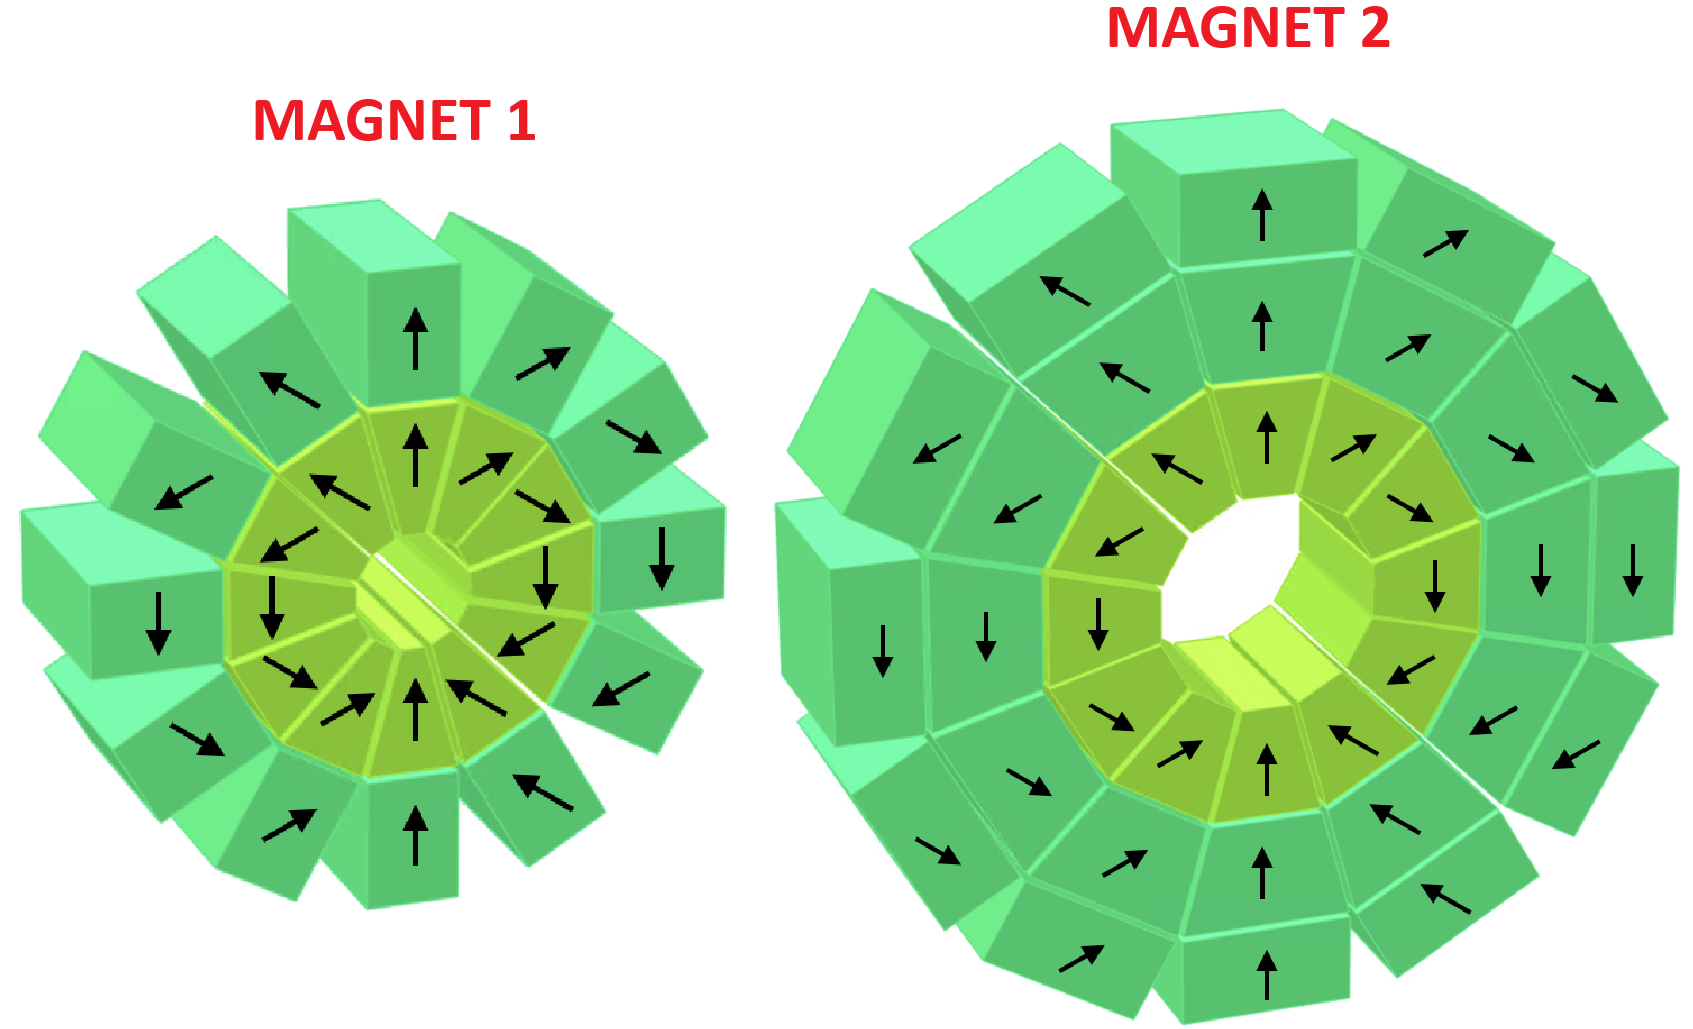
\includegraphics[width=0.85\linewidth]{permanent_magnets.png}
	\caption[Permanent magnets sketch]{Model of the two dipoles of the FOOT magnet system as built in OPERA 3D viewer. From \cite{Trigilio_2025}.}
	\label{fig:permanent_magnets}
\end{figure}
The first and the second magnets have internal diameters of $5\,\mathrm{cm}$ and $10.6\,\mathrm{cm}$, which respectively provide a maximum magnetic field intensity of $1.4\,\mathrm{T}$ and $0.9\,\mathrm{T}$ along the $y$ axis. As the $B(T)$ is oriented towards the $y$ axis and the beam follows the $z$ positive direction, the charged fragments' bending coordinate lies in the $x$ axis.\footnote{This simply derives from the Lorentz force $\vect{F_L}=q\vect{v}\times\vect{B}$. $\vect{F_L}\parallel\vect{\hat{x}}$ since $\vect{v}\parallel\vect{\hat{z}}$ and $\vect{B}\parallel\vect{\hat{y}}$.} As schematized in \autoref{fig:lifted_perm_magn}, the permanent magnets can be vertically lifted by $40\,\mathrm{cm}$ to facilitate alignment procedures, which usually do not require the presence of a magnetic field.
\begin{figure}[H]
	\centering
	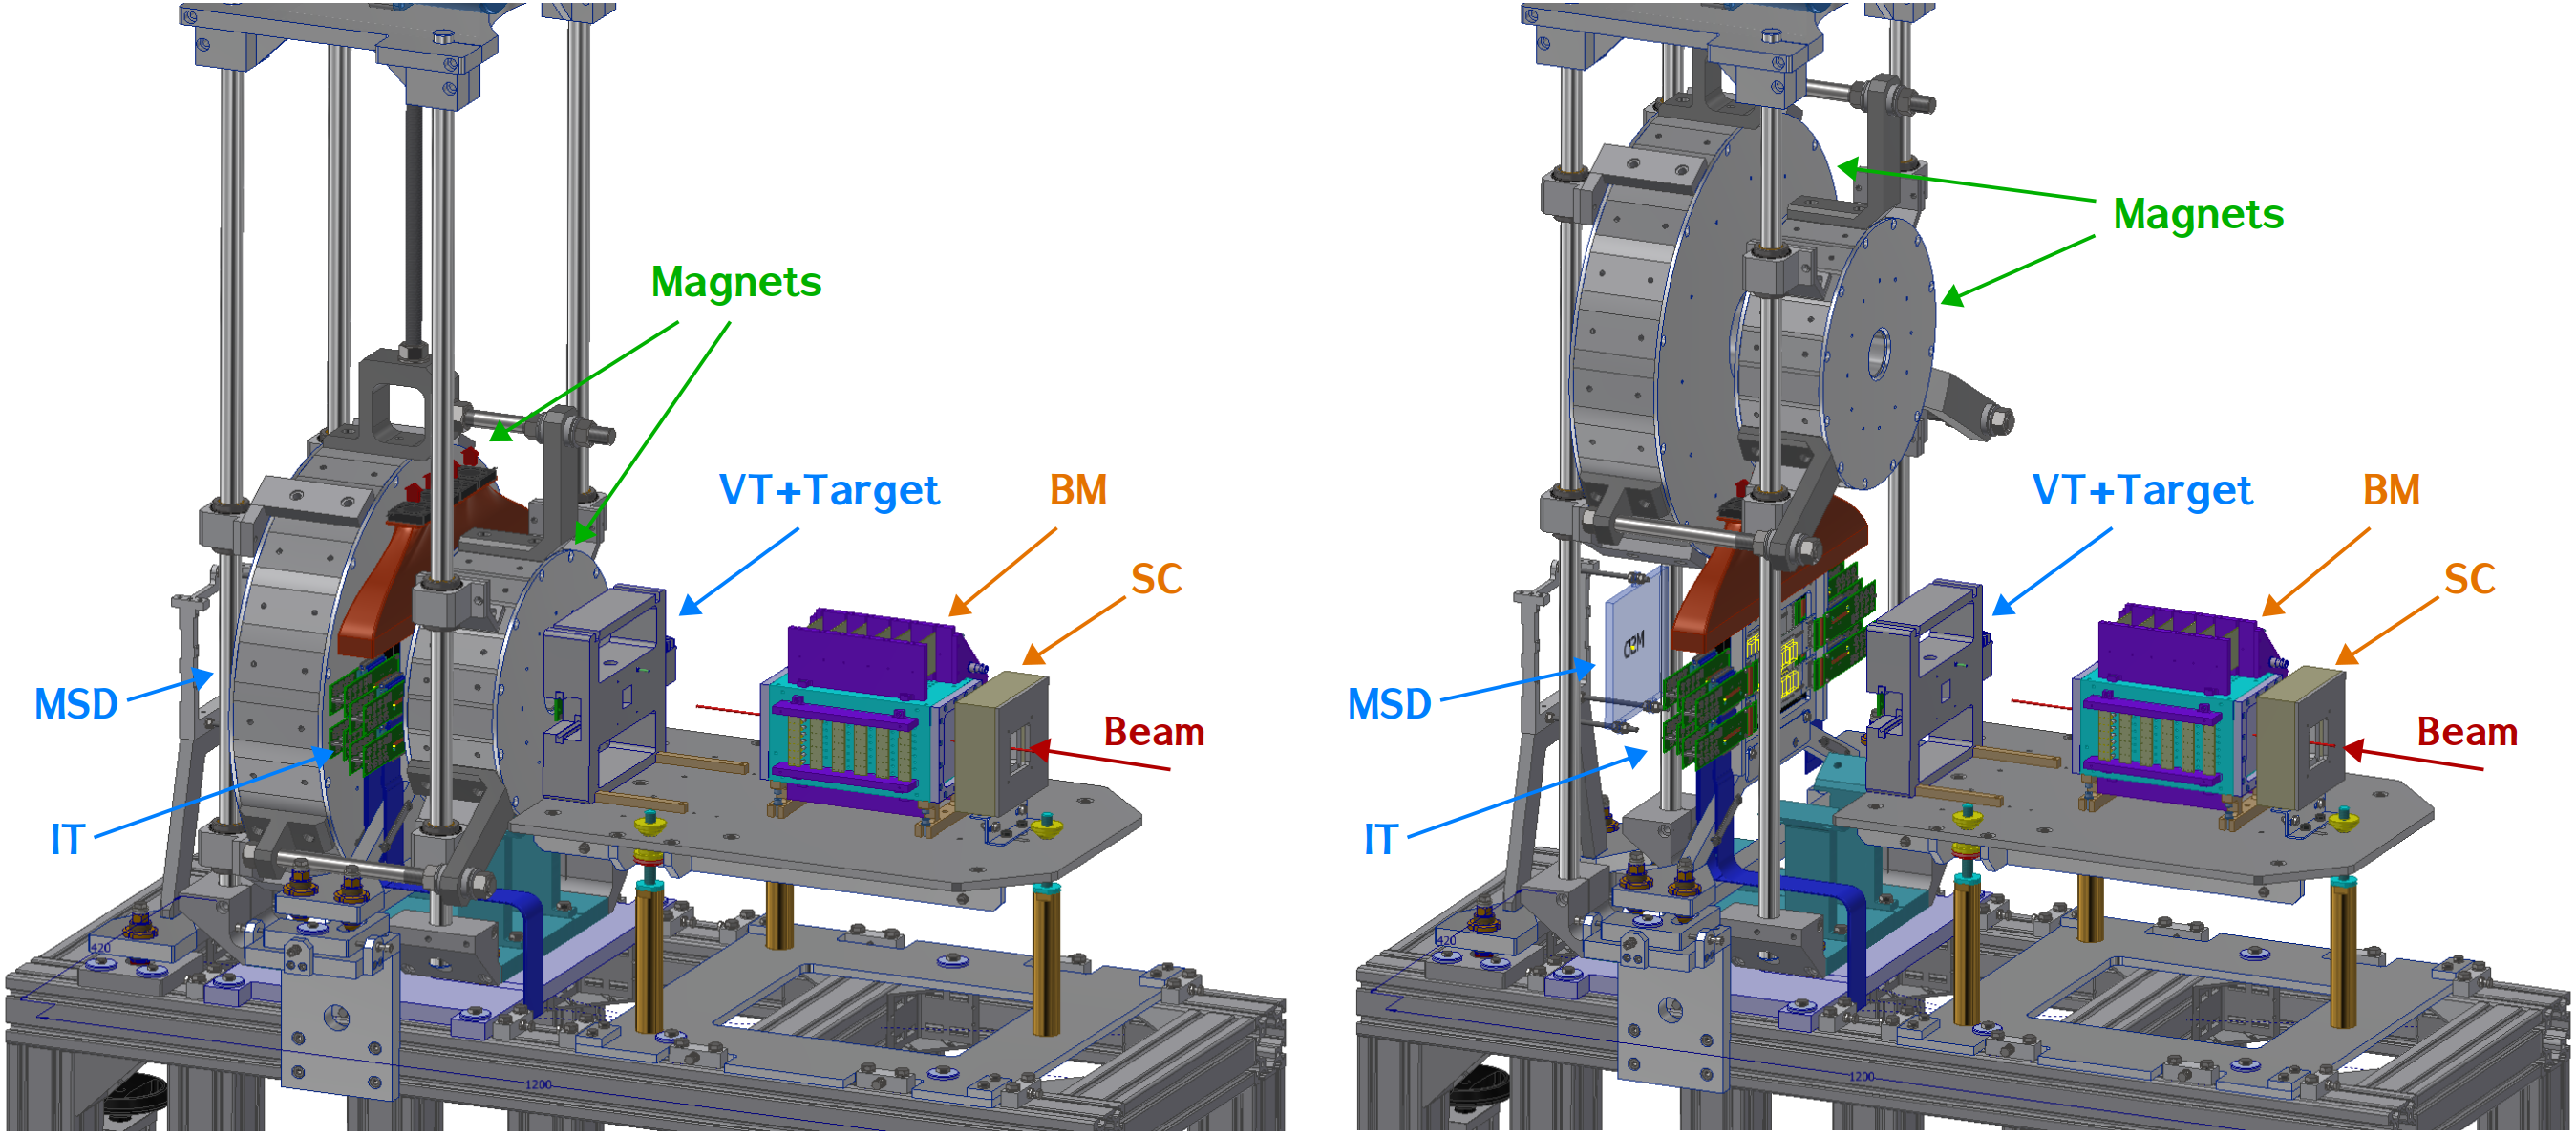
\includegraphics[width=\linewidth]{lifted_perm_magn.png}
	\caption[Vertical displacement of permanent magnets]{Technical drawing representing detectors and support structures belonging to the upstream and tracking regions, with the beam highlighted in red. The permanent magnets can be vertically displaced in (left) and out (right) of the beam line. From \cite{ZarrellaPhDThesis}.}
	\label{fig:lifted_perm_magn}
\end{figure}
\subsubsection{Microstrip Silicon Detector}\label{sssec:microstrip_silicon_detector}
To further increase the lever arm after the magnetic region, a Microstrip Silicon Detector (MSD) is located beyond the magnetic region, at approximately $30\,\mathrm{cm}$ from the target. The MSD consists of $3$ $x$-$y$ layers composed of mutually orthogonal strips providing an analog readout. Every $x$-$y$ plane (shown in \autoref{fig:msd1} (left)) is further decomposed in $2$ Single-Sided Silicon Detectors (SSSD), each providing position measurements along the $x$ and $y$ axes through orthogonally oriented strips. To minimize fragmentation and multiple coulomb scattering inside the device, each SSSD is thinned down to $150\,\mu\mathrm{m}$, half the standard thickness of SSSD tracking sensors \cite{Silvestre_2022}. As reported in \autoref{fig:msd1} (top right), the sensor active area is $9.6\times9.6\,\mathrm{cm}^2$, which guarantees the $10^\circ$ angular acceptance of FOOT electronic setup. The active surface of every SSSD is segmented in $1920$ $40\,\mu\mathrm{m}$-wide strips, each separated by an implant pitch of $50\,\mu\mathrm{m}$, whose narrowness minimizes the fragment pile-up within the same strip \cite{measurement_impact_foot}. In order to reduce experimental costs and have a more manageable data throughput, the number of readout channels is limited to $640$, meaning that only one every three strips is connected to the readout electronics, which consist of IDE1140\footnote{Previously known as VA1140.} ASIC chips bonded to the Printed Circuit Board (PCB) illustrated in \autoref{fig:msd1} (bottom right). Specifically, in each SSSD the strip analog signal is collected and amplified by $10$ IDE1140 ASICs, each possessing $64$ channels, reaching the desired $640$ channels per SSSD. Successively, the amplified signal is transferred to ADCs for the digitization.
\begin{figure}[H]
	\centering
	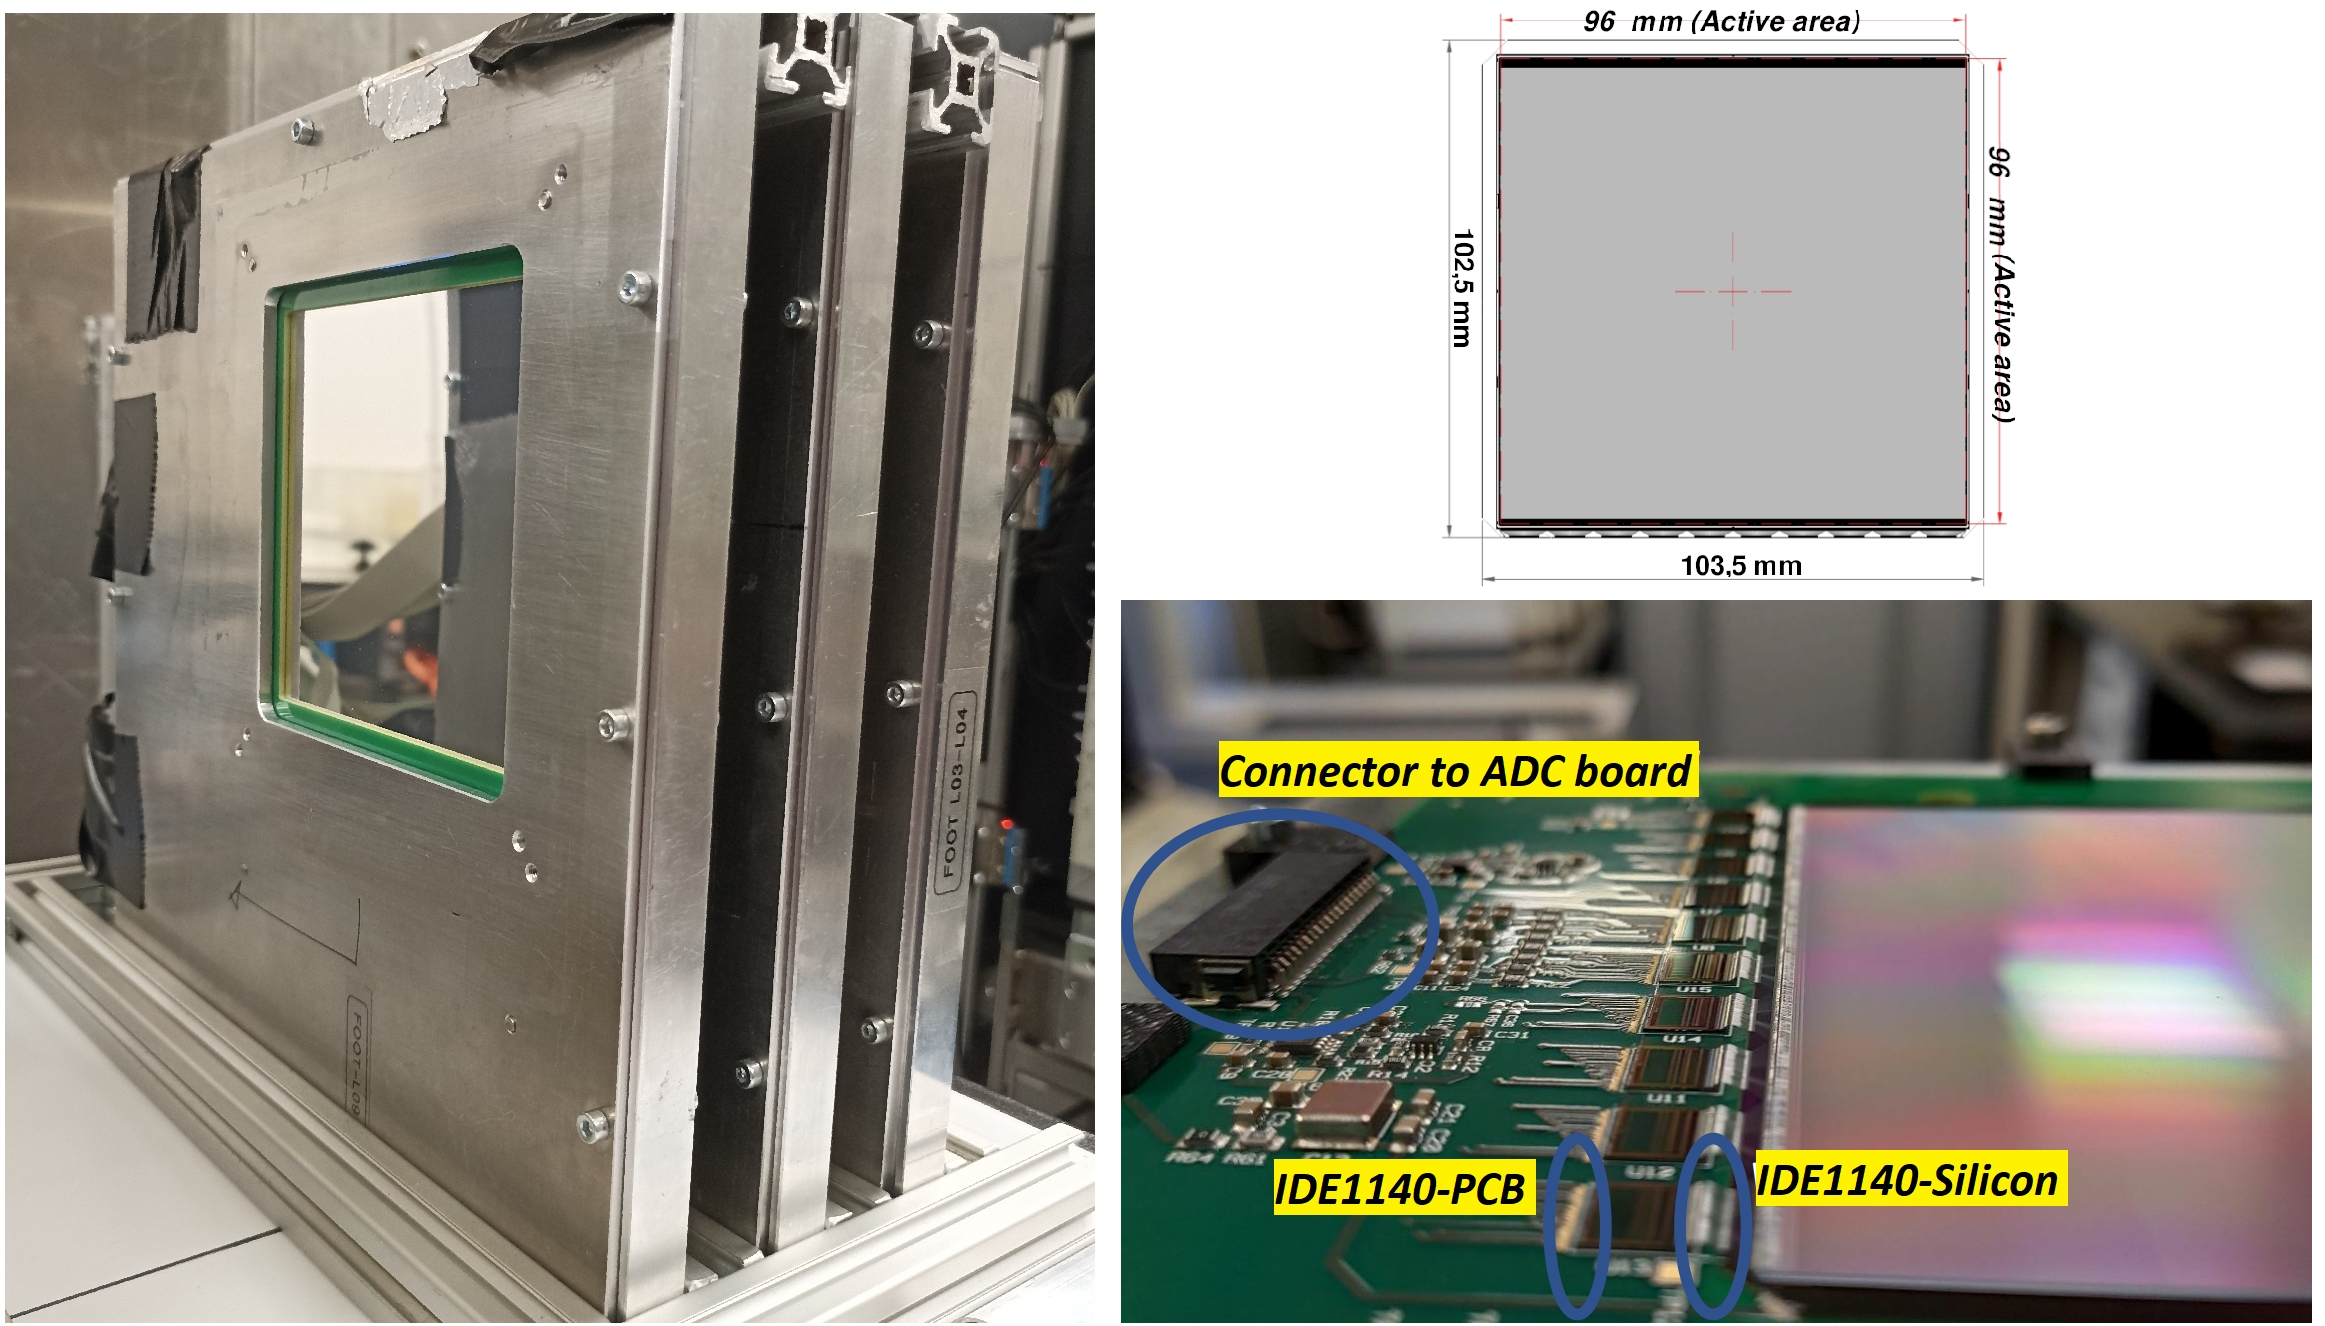
\includegraphics[width=0.95\linewidth]{msd1_jpg.jpg}
	\caption[Pictures of Microstrip Silicon Detector]{On the left, picture of the MSD detector during a data taking at the HIT facility (Heidelberg, Germany) in 2022. On the top right, technical drawing of the silicon sensor with relative dimensions. On the bottom right, PCB with the sensor-ASIC and ASIC-hybrid board wire bondings, both circled in blue on the right of the picture. The leftmost ADC board connector is also highlighted in blue. From \cite{ZarrellaPhDThesis,Silvestre_2022}.}
	\label{fig:msd1}
\end{figure}
The sketch in \autoref{fig:msd2} may be helpful to further investigate the MSD structure. In this figure, $50\,\mu\mathrm{m}$-distant floating strips separate the neighboring readout strips, the latter being $150\,\mu\mathrm{m}$ apart. Despite not being instrumented, the floating strips are still able to collect electron-hole pairs produced after particle ionization and, via capacitive coupling (the interstrip capacitance in \autoref{fig:msd2}), they share the deposited charge to the neighboring readout strips. A digital readout of $150\,\mu\mathrm{m}$-distant strips would provide a spatial resolution of $\simeq40\,\mu\mathrm{m}$, however the floating strip solution, combined with the MSD analog readout, can improve the position resolution by a factor $3$, as reported in \cite{ADRIANI199776,ALPAT2010207}.

Along with the improvement in spatial resolution, the MSD analog readout is more advantageous than the binary readout, at least for two other reasons. First, it reduces the problem of ghosts hits, that is the instrumental misidentification of particle coordinates due to triangulation ambiguities. Ghost hits represent an arduous challenge in detectors constituted by orthogonal strips like the MSD. Nevertheless, the MSD analog readout measures the value of energy deposited within the sensor rather than a mere hit/no hit information. In this way, detector hits induced by comparable energy depositions can be more easily matched and attributed to the particle that generated them, thereby reducing spatial ambiguities and, consequently, combinatorial background. Secondarily, combining the energy $\Delta E$ provided by the analog readout and the MSD thickness $\Delta x$, it is possible to evaluate the $dE/dx$ \cite{SMeroli_2011,ZUCCON200874,ALPAT2000522}, which can be used to measure the fragment charge via \autoref{eq:bethe_bloch}. The charge identification performed by the MSD is of utmost importance, as it occurs before the $\simeq1\,\mathrm{m}$ of air which separates the MSD from the ToF Wall (see \autoref{sssec:tof_wall}), where fragments could potentially undergo fragmentation in air.
\begin{figure}[H]
	\centering
	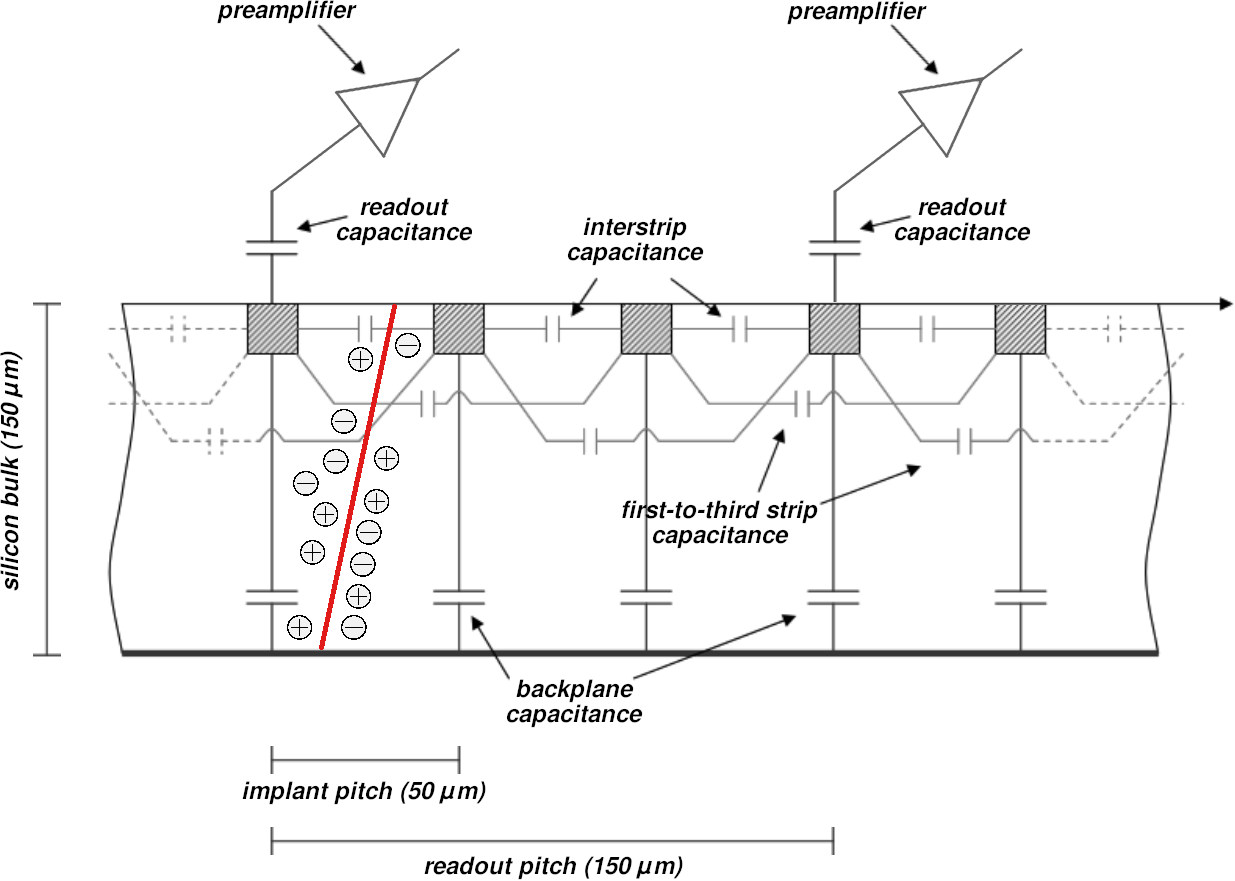
\includegraphics[width=0.95\linewidth]{msd2.png}
	\caption[Electric scheme of Microstrip Silicon Detector]{Electric scheme of MSD sensor, with its readout and floating strip structure. A charged particle trail, with the electron-hole pairs generated from ionization, is highlighted in red. From \cite{Silvestre_2022}.}
	\label{fig:msd2}
\end{figure}
\subsection{Downstream region}\label{ssec:downstream_reg}
The downstream region is the distal part of the electronic setup. It is located at $1$--$2\,\mathrm{m}$ from the target, depending on the experimental room dimensions, and provides the final timestamp of ToF as well as the fragment kinetic energy measurement.
\subsubsection{ToF Wall}\label{sssec:tof_wall}
\begin{figure}[H]
	\centering
	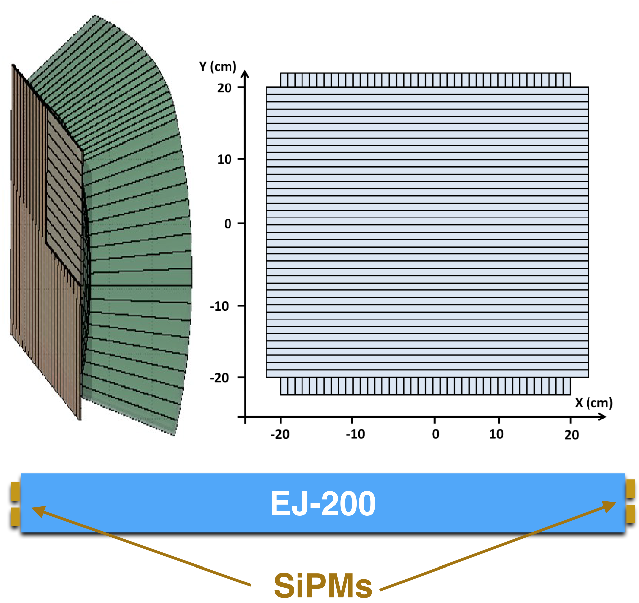
\includegraphics[width=0.55\linewidth]{TW1.png}
	\caption[Scintillating bars of ToF Wall]{At the top left, schematic view of the TW orthogonal scintillating bars, located in front of the FOOT Calorimeter. At the top right, schematized structure of TW layers. At the bottom, $1$ EJ-200 TW bar coupled with $4$ SiPMs, $2$ for each side. From \cite{9273065,Traini2019FOOT}.}
	\label{fig:TW1}
\end{figure}
The ToF Wall (TW) detector is composed of $2$ orthogonal layers of EJ-200 plastic scintillator bars \cite{ej200datasheet}, schematically illustrated in \autoref{fig:TW1} (top). Each TW layer possesses $20$ $0.3\,\mathrm{cm}$-thick, $2\,\mathrm{cm}$-wide and $44\,\mathrm{cm}$-long parallel scintillation bars, oriented either along the $x$ or the $y$ axis. The total active area of $40\times40\,\mathrm{cm}^2$ provides the desired angular acceptance of $\simeq10^\circ$ at approximately $1\,\mathrm{m}$ from the target. Combining the $2$ layers, the TW reaches a granularity of $2\times2\,\mathrm{cm}^2$, which matches the dimension of the downstream Calorimeter's crystals (see \autoref{sssec:calorimeter}) and keeps the fragment pile-up in the same bar below $1\%$ \cite{measurement_impact_foot}. The $2\,\mathrm{cm}$ bar thickness offers a compromise between an high light yield and a low fragmentation probability inside the bars. Moreover, the scintillator plastic material guarantees fast signals, fundamental for the ToF determination. As shown in \autoref{fig:TW2} (left), each TW bar is wrapped in reflective aluminum \cite{MORROCCHI2019116,CIARROCCHI201978} to maximize light collection efficiency and to guide more effectively the luminous signal towards $4$ SiPMs (MPPC by Hamamatsu \cite{sipmTW}), positioned at the bar extremities in groups of $2$, as sketched in \autoref{fig:TW1} (bottom). Each SiPM is characterized by a $3\times3\,\mathrm{mm}^2$ sensor area with a microcell pitch of $25\,\mu\mathrm{m}$ and by a large number of pixels (\num{14400}), which guarantees a dynamic range sufficiently wide to measure energy releases from proton to oxygen particles at different kinetic energies. Additionally, every SiPM pair located at the TW bar ends is biased and readout by a single channel that digitizes signals at a rate of $3$--$4\,\mathrm{GS/s}$, employing the WaveDAQ system \cite{GALLI2019399} already mentioned in \autoref{sssec:start_counter} for the SC. To reduce background noise from environmental light, the TW active area is further covered by the darkening black tape pictured in \autoref{fig:TW2} (right) \cite{MORROCCHI2019116,CIARROCCHI201978}.
\begin{figure}[H]
	\centering
	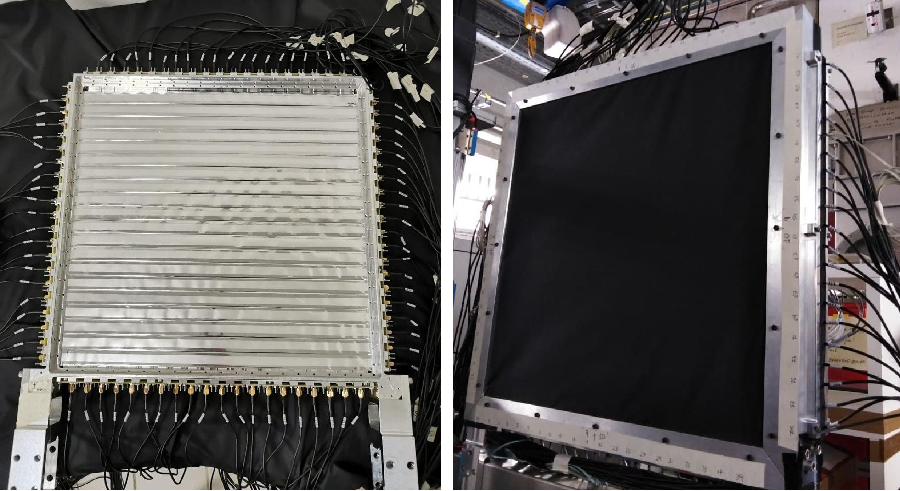
\includegraphics[width=0.98\linewidth]{TW2.png}
	\caption[ToF Wall pictures]{On the left, TW scintillating bars with wire connections devoted to readout. On the right, a closed TW with black shielding to screen the environmental background light. From \cite{RidolfiPhDThesis}.}
	\label{fig:TW2}
\end{figure}
The TW measures the ToF final timestamp and the particles' deposited energy $\Delta E$. The former allows to calculate the whole ToF, since the ToF initial timestamp is known from the preceding SC measurement. Conversely, the $\Delta E$ enables to identify the particle charge $Z$ \cite{KRAAN2020162422,GALLI2019399} using the \autoref{eq:bethe_bloch}, guaranteeing the redundant $Z$ evaluation previously performed in the MSD (see \autoref{sssec:microstrip_silicon_detector}). The TW-MSD charge identifications are of paramount importance also for the fragment mass reconstruction, as discussed in (?? global analysis). Indeed, the reconstruction algorithm computes the rigidity $p/Z$ of a particle rather than the momentum $p$. Thus, a precise estimation of $p$ can only stem from an accurate $Z$ identification. Finally, the previous studies \cite{KRAAN2021165206,KRAAN2020162422} showed that the TW is capable of achieving the FOOT required resolutions (see \autoref{sec:electronic_setup}) on both ToF and $\Delta E$.

The TW provides further assistance to the global reconstruction of particle tracks. Indeed, when a particle traverses the orthogonal scintillating bars, the charge deposition produces a cluster of energy that delineates a ``TW point'' from the $x$-$y$ bar intersection. The TW point can then be used as an additional tracking point. Although the $2\times2\,\mathrm{cm}^2$ granularity of the scintillation bars results in a spatial uncertainty on the TW point larger by a factor $100$--$1000$ than that of silicon detector hits, the additional TW point improves track reconstruction and, consequently, reduces the spatial uncertainties on the particle trajectory, as demonstrated in \cite{MORROCCHI2019116}.
\subsubsection{Calorimeter}\label{sssec:calorimeter}
The furthest detector in the electronic setup is the FOOT electromagnetic Calorimeter (CALO), an inorganic scintillator designed to measure the fragment kinetic energy $E_\text{kin}$ by fully stopping the crossing fragments. The $E_\text{kin}$ is a fundamental variable employed in \autoref{eq:a2} and \autoref{eq:a3} to estimate particle masses. Naturally, the final fragment $E_\text{kin}$ is given by the sum of $\Delta E$ deposited in the MSD, in the TW and in the CALO:
\begin{equation}
	E_\text{kin}=\Delta E_{MSD}+\Delta E_{TW}+\Delta E_{CALO}.
	\label{eq:kinetic_energy}
\end{equation}

The CALO consists of dense BGO (\ce{Bi4Ge3O12}, density $\rho=7.13\,\mathrm{g/cm}^3$) crystals, which guarantee a large stopping power and a good light yield of $\simeq10\,\mathrm{photon/keV}$, fulfilling the uncertainty requirements on $E_\text{kin}$ presented in \autoref{sec:electronic_setup}. As shown in \autoref{fig:calo} (left), the $320$ BGO crystals are arranged in a parabolic-like shape and are mechanically separated into $3\times3$ modules, as illustrated in \autoref{fig:calo} (right). Each BGO crystal has a truncated-pyramid shape with a length of $24\,\mathrm{cm}$ and an extension of the front and back surfaces of respectively $2\times2\,\mathrm{cm}^2$ and $3\times3\,\mathrm{cm}^2$, similar to the TW granularity (see \autoref{sssec:tof_wall}). The selected BGO shape and dimensions minimize secondary fragmentations, limiting the fragmentation pile-up probability within a single crystal below $1$--$2\%$, depending on the beam energy and the experimental room setup configuration. Moreover, the $24\,\mathrm{cm}$-depth was chosen to minimize energy leakages caused by neutrons escaping the CALO.
\begin{figure}[H]
	\centering
	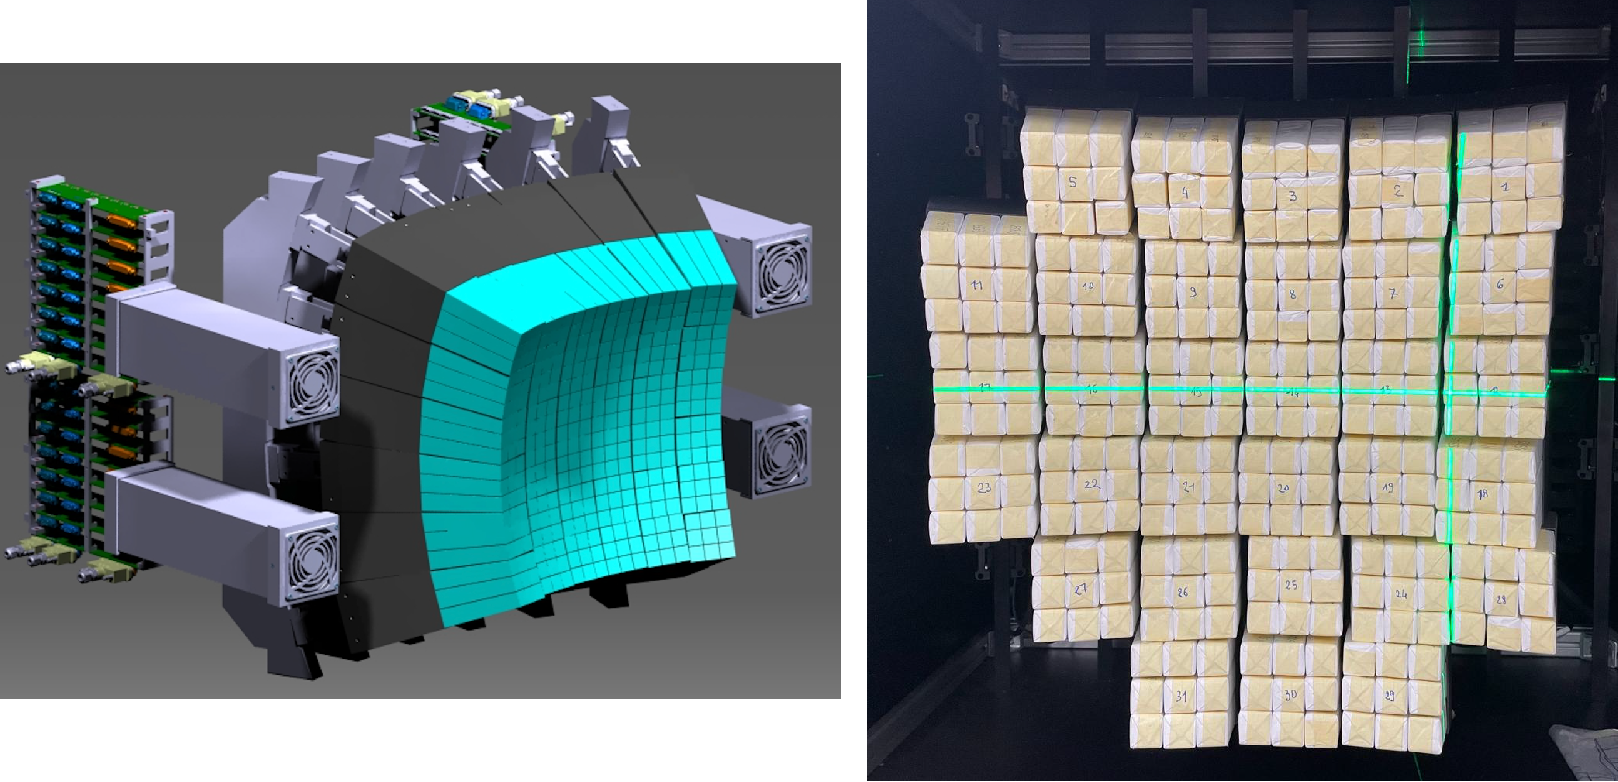
\includegraphics[width=0.98\linewidth]{calo.png}
	\caption[Calorimeter]{On the left, the CALO technical drawing. On the right, picture of the BGO crystal modules during assembling. A laser-based alignment procedure is also displayed \cite{Bartosik_2025}.}
	\label{fig:calo}
\end{figure}
As shown in \autoref{fig:calo2} (left), each BGO back surface is optically coupled with $25$ SiPMs that collect scintillation light through an active area of $2\times2\,\mathrm{cm}^2$ and a microcell pitch of $15\,\mu\mathrm{m}$, ensuring a linear response up to $10\,\mathrm{GeV}$ and meeting the $E_\text{kin}$ resolution requirements \cite{measurement_impact_foot}. A $5\times5$ matrix of $25$ SiPMs is pictured in \autoref{fig:calo2} (right). Every SiPM is connected to a readout board interfaced with the WaveDAQ system \cite{GALLI2019399}, the same readout used for SC and TW.
\begin{figure}[H]
	\centering
	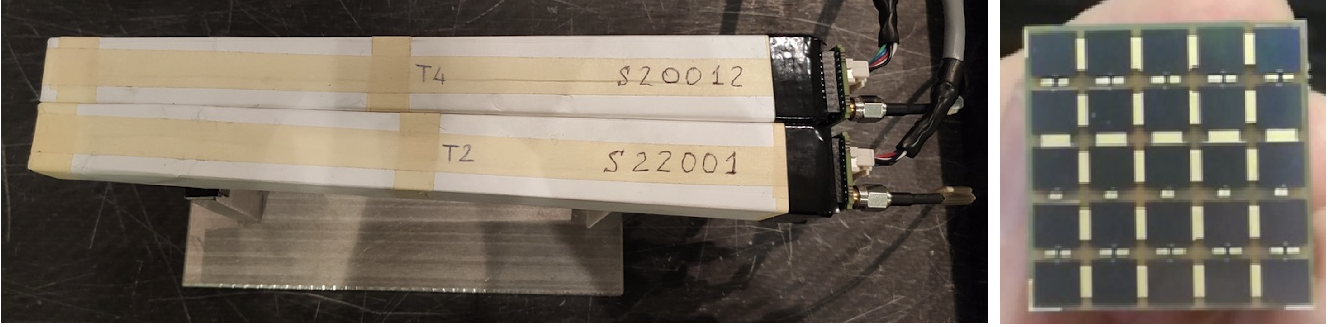
\includegraphics[width=0.98\linewidth]{calo2.png}
	\caption[Calorimeter crystals coupled with SiPMs]{On the left, module of two BGO crystals with SiPMs attached to their back end and relative readout wiring. On the right, picture of a CALO SiPM \cite{Bartosik_2025}.}
	\label{fig:calo2}
\end{figure}
Despite the BGO large density and good light yield, the particle showers produced by traversing fragments may be not fully contained within the CALO, especially at higher energies, when hadronic processes become significant. Indeed, at the largest energies of $700$--$800\,\mathrm{MeV/u}$, relevant for SRP applications, the particle showers reveal both the electromagnetic and hadronic components. While the first is not problematic for an electromagnetic calorimeter like FOOT's CALO, the second leads to unwanted energy leakages, which inevitably worsen the $E_\text{kin}$ measurement performance. Substituting the electromagnetic CALO with an hadronic calorimeter is also unfeasible, not only for financial affordability reasons, but also for its superior dimensions, which would definitively discard the electronic setup's compactness, one of FOOT design priorities. Nevertheless, the FOOT CALO performs well between $200$--$400\,\mathrm{MeV/u}$ \cite{measurement_impact_foot,UbaldiPhDThesis}, as electromagnetic mechanism overwhelm hadronic ones at such energies. This is due to the fact that hadronic processes are inherently connected to the pion ($\pi^{\pm}$, $\pi^0$) production threshold, whose energy values range between $280$--$290\,\mathrm{MeV/u}$.

Even at lower energies, there is still one pending challenge: neutrons. Indeed, at any energy, fragmentation processes induce secondary neutron emissions, which cannot be directly measured by the electronic setup. Escaping neutrons carry away undetectable kinetic energy, introducing systematic uncertainty on the $E_\text{kin}$ resolution. To address this predicament, the FOOT Collaboration is currently aiming to develop a novel neutron detector \cite{Zarrella_2024} capable of tracking them and measuring their kinetic energy, which would represent a breakthrough in neutron-induced risk assessment. At present, a promising neutron tracker that could be potentially integrated in the FOOT apparatus is being developed in the RIPTIDE experiment, as reported in \cite{Lanzi_2026}.
\subsection{Trigger and Data Acquisition System}\label{ssec:tdaq_electronic_setup}
In the forthcoming paragraphs, a general overview of Trigger and Data AcQuisition (TDAQ) concepts is provided, which lays the foundations for the subsequent description of the FOOT TDAQ architecture.
\subsubsection{General concepts of TDAQ systems}\label{ssec:tdaq_general_info}
The meticulous management of the event acquisition chain is crucial in multiple-subdetector experiments like FOOT, where signal synchronization plays a fundamental role to assure that the event fragments collected by the various detectors are correctly matched to the same physics event. For this reason, the TDAQ acquires data only when all detectors are ready (i.e, are not in a busy state), otherwise information losses or data mixing could potentially lead to corrupted events that are impossible to handle during offline analysis. Hence, any raised busy signal prevents the trigger generation and distribution, blocking the data acquisition. Once the busy state is cleared, the TDAQ waits for the forthcoming trigger, which is generated once an interesting physics event is deemed accepted by the trigger decision logic. The time elapsing between the physics signal formation and the consequent trigger generation and distribution is called latency, and must be kept as low as possible.
\begin{figure}[H]
	\centering
	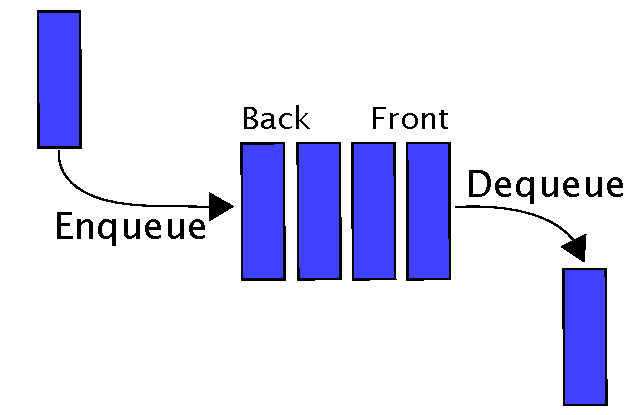
\includegraphics[width=0.45\linewidth]{fifo.pdf}
	\caption[FIFO queue]{Representation of a FIFO queue \cite{fifo_image}.}
	\label{fig:fifo}
\end{figure}
Another fundamental concept in TDAQ systems is the balance between deadtime $\tau$, physical rate $f$ and DAQ output rate $\nu$ \cite{RidolfiPhDThesis}. First, the deadtime $\tau$ is the time needed to fully process an event until its final storage on disk. Second, the physical rate $f$ is the frequency of the physics event (e.g., in FOOT it could be a the beam rate arrival in the SC). Third, the DAQ output rate $\nu$ is the data throughput, that is the real acquisition rate of the experiment. Although the minimization of $\tau$ is often possible, doing so entails high costs and technical constraints that can rarely be overcome. Hence, to avoid bottlenecks between the incoming physical rate $f$ and the DAQ output rate $\nu$, the preferred solution is to decouple the event ingestion from their output processing with buffers. A buffer is a memory device that stores data temporarily while it is being moved from one place to another. For instance, a common way to handle data buffers is through the FIFO (First In, First Out) manipulation, where the oldest (first) entry is processed first as illustrated in \autoref{fig:fifo}.

Even if an average input rate can be defined, in real-world conditions there can be short data bursts where data arrives almost simultaneously, instantaneously incrementing the input rate. Such rate fluctuations may overload the data acquisition system, increasing the probability of raising DAQ busies (to give the system time to complete the acquisition) and, consequently, data losses. For this reason, buffers are inserted in the whole DAQ architecture to temporarily absorb the excess events, preserving the overall detection efficiency. This duty is usually referred to as ``derandomization'', because a random input flow is converted into a smoother output data stream. The buffer depth must be carefully designed considering data dimensions and DAQ processing rates.
\subsubsection{The FOOT TDAQ}\label{ssec:tdaq_foot}
\begin{figure}[H]
	\centering
	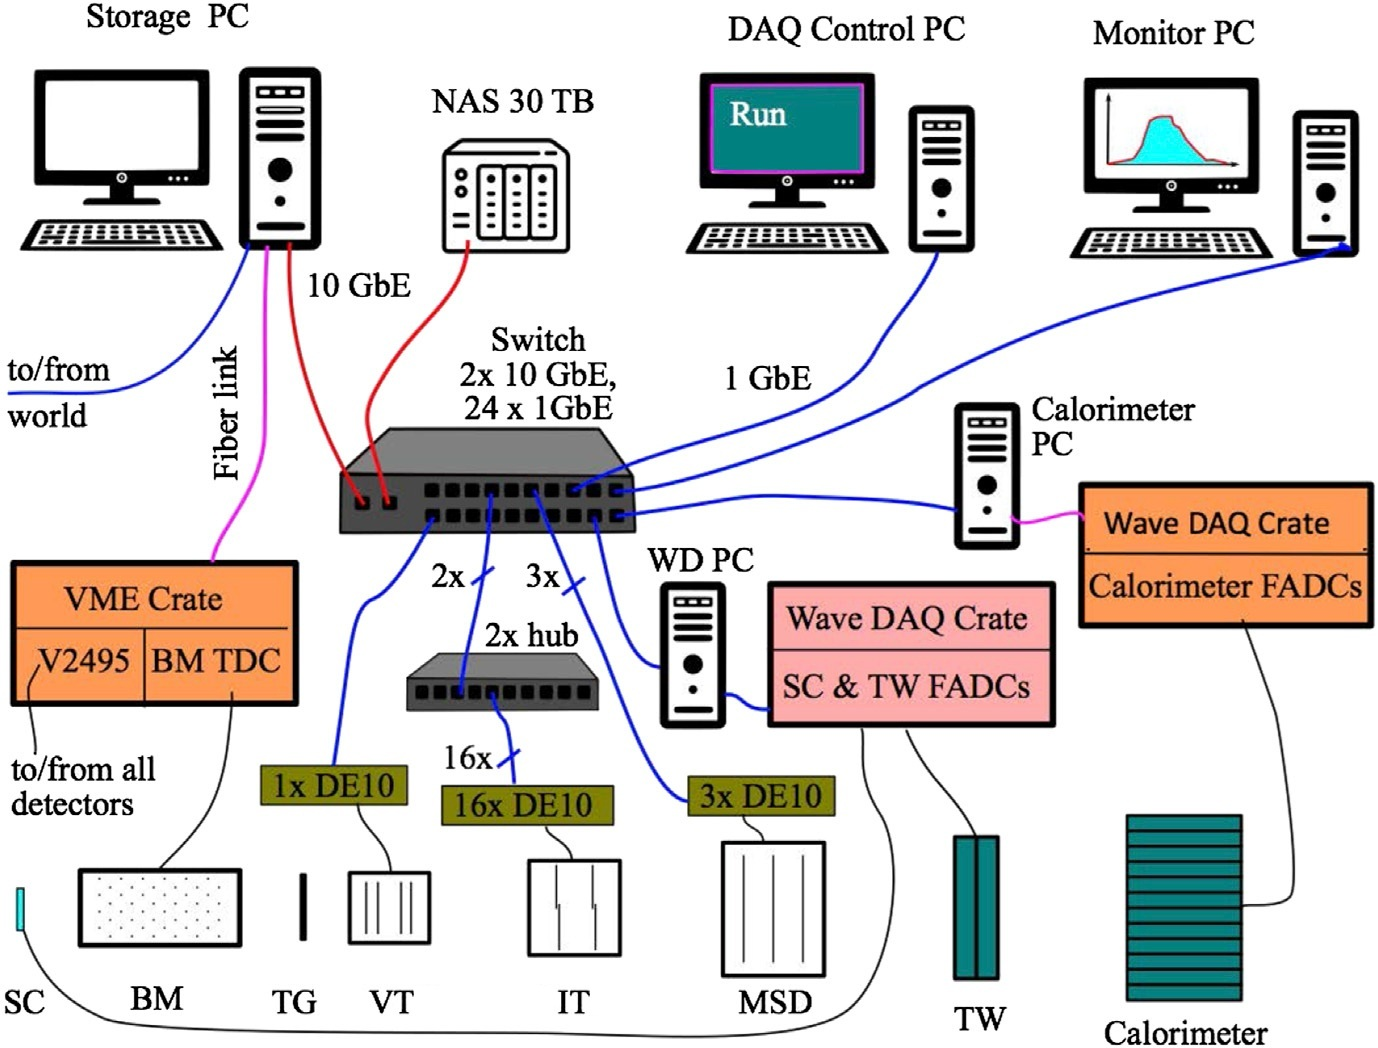
\includegraphics[width=0.8\linewidth]{tdaq.jpg}
	\caption[FOOT Trigger and Data Acquisition System]{Scheme of FOOT Trigger and Data Acquisition System. Adapted from \cite{measurement_impact_foot}.}
	\label{fig:tdaq}
\end{figure}
The FOOT Trigger and Data Acquisition (TDAQ) system (see \autoref{fig:tdaq}) is the comprehensive infrastructure that handles all the steps from processing the signal generation inside a detector to acquiring and saving on permanent storage the triggered experimental data comprising information of physical interest. To achieve this, the TDAQ encompasses various architectures including the front-end electronics (i.e., the closest element to the detector devoted to signal amplification and digitization), boards dedicated to distribute trigger and busy signals (which follow a different path from experimental data), communication links such as Ethernet, USB and optical fibers and devices like Linux PCs, standard VME crates and custom FPGAs. In addition, the TDAQ correctly manages the event building chain, which ensures that the experimental data coming from detectors of different kind is correctly parsed with the respective metadata, such as timestamp, event number and tag strings. The FOOT TDAQ architecture is based on a TDAQ system used in the ATLAS experiment at LHC (Large Hadron Collider, CERN) \cite{Jenni_616089}, and it is currently maintained by the University and the INFN section of Bologna \cite{foot_site}.

As shown at the center of \autoref{fig:tdaq}, a network Switch collects the detector data sending it forward to the Storage PC, which manages the whole acquisition on a SSD (Solid-State Drive) with a writing speed of $\simeq400\,\mathrm{MB/s}$. The Switch is connected to $20$ DE10-Nano or DE10 Terasic boards cabled to VT, IT, MSD and the WaveDAQ for SC, TW and CALO via $1\,\mathrm{Gb}$ Ethernet connection. The Switch $10\,\mathrm{Gb}$ Ethernet ports are instead reserved to the Storage PC and the NAS (Network Attached Storage). The Storage PC is also wired to the VME Crate housing a V2495 board, that is the FOOT central trigger module, managing the distribution of trigger and busy signals across all detectors. Moreover, the VME Crate hosts a CAEN V2718 board, which connects the VME Crate with the BM electronics (TDC (Time to Digital Converter) and discriminators) \cite{UbaldiPhDThesis,ZarrellaPhDThesis}. While all these components are installed into the experimental room, a Control PC is remotely managed in the control room. From the Control PC it is possible to start/stop runs and control/configure other system nodes. Through another Monitor PC, online monitoring activities are performed.

FOOT employs two main trigger logics: the Minimum Bias Trigger (MBT) and the Fragmentation Trigger (FT). The MBT is valid when an incoming ion enters the SC, while the FT activates when the FT holds true and the TW registers a pulse height compatible with a fragmentation event. Both the BMT and FT are raised by the WaveDAQ system and distributed across the subdetectors by the V2495 board. Due to beam constraints and to the slow reading of M28 sensors, the current data acquisition rate of the FOOT experiment is $\simeq1\,\mathrm{kHz}$.
\section{Emulsion setup}\label{sec:emulsion_setup}
Although emulsion chambers have been superseded by electronic detectors since the 1960s \cite{Ariga2020}, they are still used today in particle physics for multiple reasons, such as compactness, high tracking accuracy (sub-micrometric) and fast responses \cite{measurement_impact_foot}. Before FOOT, in the context of nuclear fragmentation, experience with emulsion chambers was gained at HIMAC in Chiba where, in order to study the fragmentation of \ce{^{12}C} ions at $400\,\mathrm{MeV/u}$, a detector composed of alternating layers of polycarbonate (Lexan, emulating human tissues) and emulsion films was employed \cite{articleNakamura,articleLellis1,articleLellis2}.

The FOOT Emulsion Setup (ES) is a nuclear emulsion spectrometer used to efficiently detect light nuclear fragments ($Z\leq2$), whose scattering angle ($\lesssim70^\circ$) is too large compared to the angular acceptance of the electronic setup. An compact emulsion chamber was specifically chosen by the FOOT Collaboration to circumvent the construction challenges of large-angular-acceptance calorimeters, characterized by high costs and low portability.

The FOOT ES is located after the Start Counter (SC) and the Beam Monitor (BM) subdetectors, as illustrated in \autoref{fig:position_es}. During the ES data taking campaigns, the SC and the BM are included just for monitoring purposes: their DAQ (see \autoref{ssec:tdaq_foot}) is completely decoupled from the ES data acquisition. Indeed, nuclear emulsions can be considered complete, self standing experiments, requiring neither real-time electronic DAQ nor power supply \cite{instruments2020007}.
\begin{figure}[H]
	\centering
	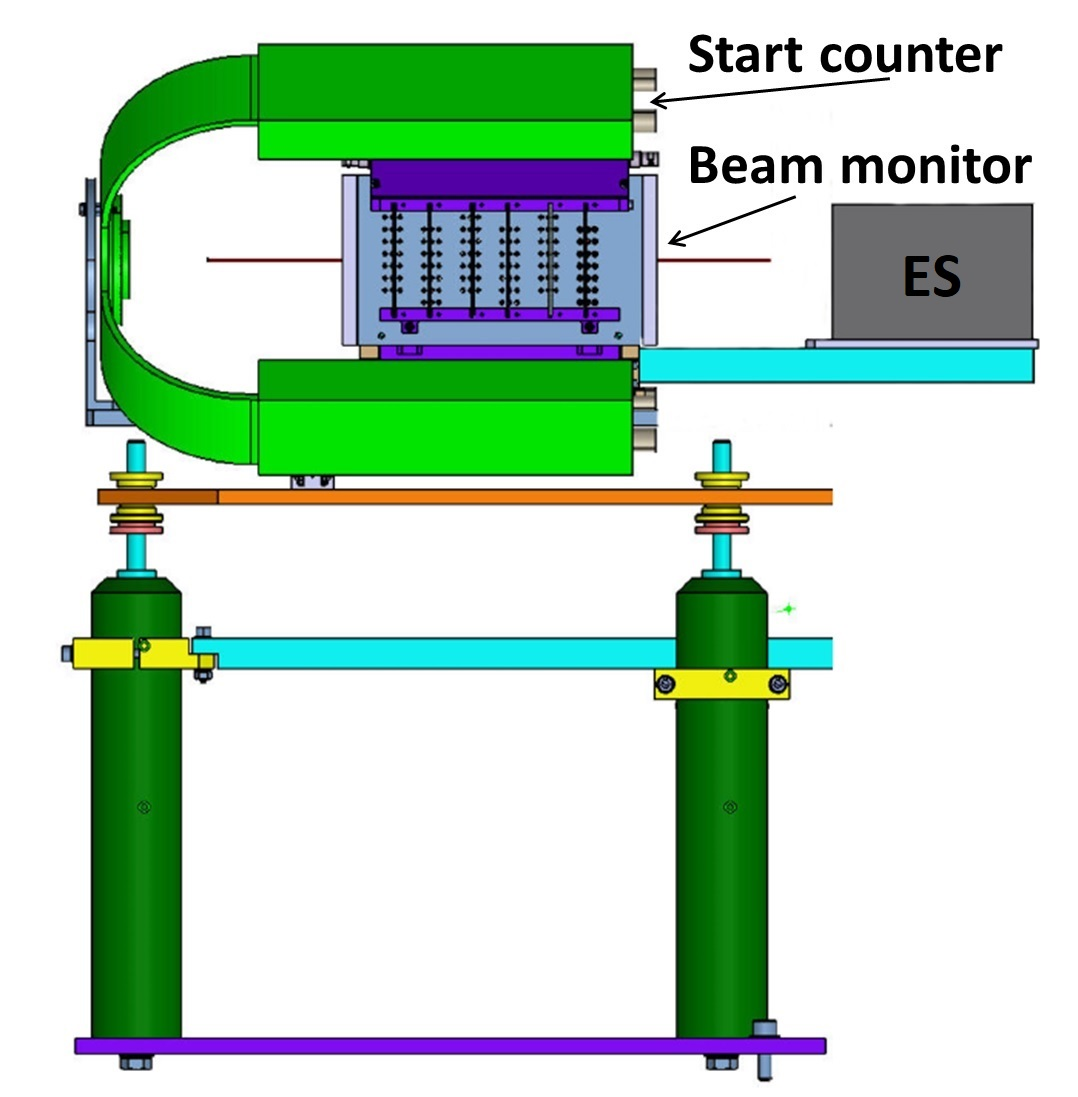
\includegraphics[width=0.55\linewidth]{position_es.jpg}
	\caption[Emulsion setup position]{Location of the ES within the FOOT experimental apparatus \cite{foot_cdr}.}
	\label{fig:position_es}
\end{figure}
A single sensitive module of the FOOT ES consists of $2$ $70\,\mu\mathrm{m}$-thick \ce{AgBr} layers, which are separated by a plastic slab of $210\,\mu\mathrm{m}$ thickness as schematized in \autoref{fig:trail_es}. Specifically, the $2$ sensitive regions are composed of \ce{AgBr} fine crystal grains of $0.2\,\mu\mathrm{m}$ diameter uniformly dispersed in a transparent gelatin binder.
\begin{figure}[H]
	\centering
	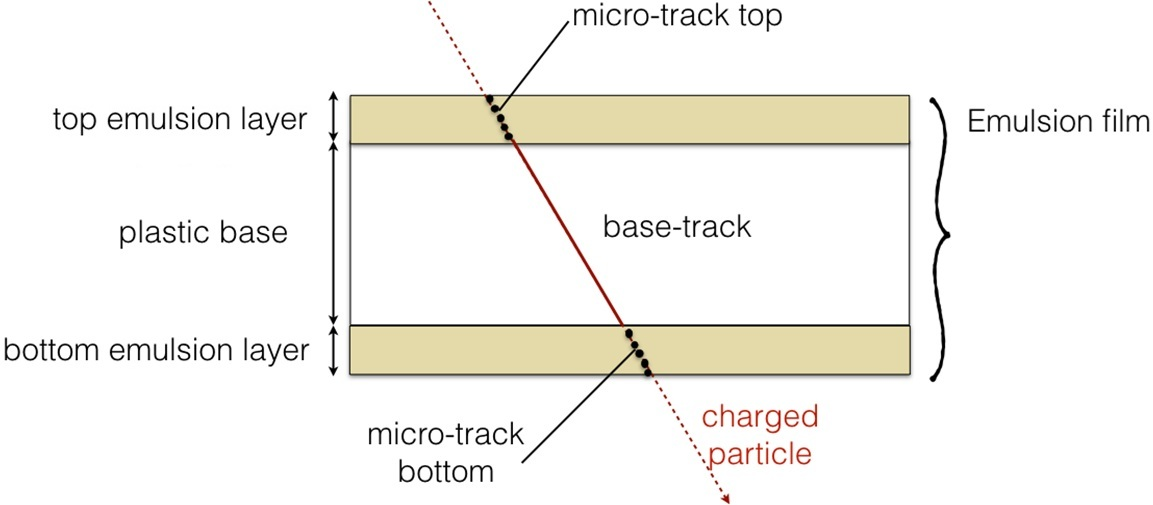
\includegraphics[width=0.7\linewidth]{trail_es.jpg}
	\caption[Emulsion setup sensitive section]{Schematic representation of the ES sensitive section. Micro- and base- tracks are also illustrated. Adapted from \cite{foot_cdr}.}
	\label{fig:trail_es}
\end{figure}
The signal formation in nuclear emulsions resembles, \textit{mutatis mutandis}, the development of a photographic plate, as explained in \cite{KolanoskiBook}. Firstly, when a charged particle traverses the \ce{AgBr} layers, the energy deposit generates electron-hole pairs, since \ce{AgBr} crystals are semiconductors with a band gap of $2.6\,\mathrm{MeV}$. The generated electrons diffuse through the crystal and are primarily trapped by lattice defects at the crystal surface. Conversely, the ionized, positively charged silver ions, usually sitting at interstitial sites,\footnote{Interstitial sites are the empty spaces or gaps situated between the atoms/ions composing the crystalline lattice.} can be attracted by negatively charged defects and become neutralized. The reiteration of this process at the same lattice defect induces the formation of metallic silver clusters, usually consisting of three or four atoms. These silver clusters constitute the so-called latent image centers, which become visible only after a ``development'' process that augments the number of cluster atoms by a factor $10^8$--$10^10$ \cite{KolanoskiBook,TANI2020164163}. After the development, the enlarged silver grains (with an increased diameter of $0.6\,\mu\mathrm{m}$) mark the charged particle trajectory with a spatial resolution better than $1\,\mu\mathrm{m}$. An picture of developed silver grains is shown in \autoref{fig:emulsiontrackpic} (left), while a pion track reconstructed in the AEgIS \cite{KIMURA2013325} nuclear emulsion is illustrated in \autoref{fig:emulsiontrackpic} (right).
\begin{figure}[H]
	\centering
	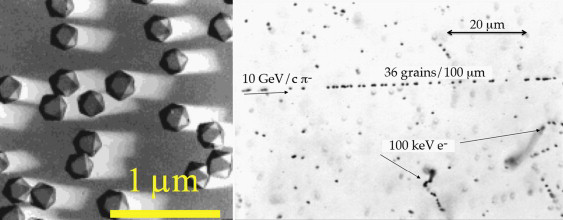
\includegraphics[width=0.98\linewidth]{emulsion_track.png}
	\caption[\ce{AgBr} crystals and tracks in an emulsion layer]{On the left, picture of \ce{AgBr} crystals in an emulsion layer taken with a Scanning Electron Microscope (SEM). On the right, track of a minimum ionizing pion with a momentum of $10\,\mathrm{GeV/c}$. From \cite{KolanoskiBook}.}
	\label{fig:emulsiontrackpic}
\end{figure}
Successive to the development process, the FOOT emulsion chamber is scanned by an automated system already adopted in the OPERA experiment \cite{ARMENISE2005261,ARRABITO2006578} and in the FIRST project \cite{PhysRevC.93.064601}, which employs a cluster-spotting software to reconstruct particle trajectories. A straight sequence of clusters in a single \ce{AgBr} layer defines a ``micro-track''. Two aligned micro-tracks belonging to the same ES sensitive module form a ``base-track''. Micro- and base- tracks, schematized in \autoref{fig:trail_es}, are then combined across all the ES films to generate ``volume-tracks''. The volume-track thickness is a variable sensitive to the ionization density, therefore it is used to perform charge identification, as reported in \autoref{ssec:ChargeIdentificationRegion}.

The FOOT ES consists of $3$ stratified sections composed of emulsion films alternated with passive materials, as illustrated in \autoref{fig:structure_es}. The three ES sections are:
\begin{itemize}
	\item the Interaction and Vertexing Region (see \autoref{ssec:InteractionandVertexingRegion});
	\item the Charge Identification Region (see \autoref{ssec:ChargeIdentificationRegion});
	\item the Momentum Measurement Region (see \autoref{ssec:MomentumMeasurementRegion}).
\end{itemize}
The purposes of each Region are detailed in the following sections.
\begin{figure}[H]
	\centering
	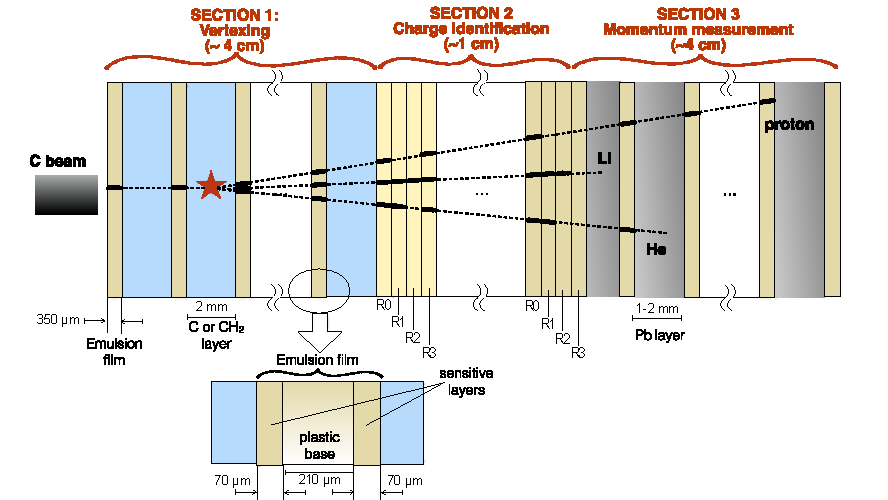
\includegraphics[width=0.98\linewidth]{structure_es.pdf}
	\caption[Emulsion setup inner structure]{Schematic representation of the FOOT ES structure. The relevant detector parts are explained in the text. Adapted from \cite{foot_cdr}.}
	\label{fig:structure_es}
\end{figure}
\subsection{Interaction and Vertexing Region}\label{ssec:InteractionandVertexingRegion}
The Interaction and Vertexing Region consists of various cells made of \ce{C} or \ce{C2H4} (the targets of FOOT experiment) alternated with emulsion films, as illustrated in \autoref{fig:structure_es}. The length of this section is adjusted at each data taking campaign to maximize detection efficiency for each beam-target-energy combination. The interaction between the primary ion and the cells of this section produces secondary fragments which are tracked and detected in the downstream sections. In addition, the sensitive layers of this section allow to retrieve the positions of interaction vertices.
\subsection{Charge Identification Region}\label{ssec:ChargeIdentificationRegion}
Inside nuclear emulsion films, Minimum Ionizing Particles (MIPs, see \autoref{ssec:bethe_bloch}) generate thin tracks whose grain density is approximately $30$--$50\,\mathrm{grains}$ every $100\,\mu\mathrm{m}$. Particles with higher ionizing power produce a grain density saturation that hinders the charge identification of secondary fragments. To circumvent this, special thermal treatments are applied to the emulsion chamber after the beam exposure but before the chemical development. These thermal procedures induce a ``fading'' effect which partially erases the saturating trails of charged particles, enlarging the overall dynamic range of the FOOT emulsion chamber as previously proved in \cite{ionChargeSep,articleLellis1,articleLellis2} previous works.

The Charge Identification Region aims to identify the charge of \ce{H}, \ce{He} and \ce{Li} fragments using nine detection cells, each composed of four emulsion films (sections from R0 to R2 are shown in \autoref{fig:structure_es}). After applying to each emulsion a different thermal treatment, the grain densities of particle tracks are extrapolated to define four volume-track variables. The correlation of these volume-track variables finally allows to measure the fragment charges.
\subsection{Momentum Measurement Region}\label{ssec:MomentumMeasurementRegion}
The Momentum Measurement Region is dedicated to the momentum $p$ measurement. It consists of emulsion films interleaved with passive material (\ce{Pb} is shown in \autoref{fig:structure_es}, but Lexan and \ce{W} can be employed as well), used to stop the crossing fragments as in the Calorimeter (see \autoref{sssec:calorimeter}). To measure fragments' momentum, two methods are used. The first is the range technique, which provides an estimate of the momentum studying the correlation between range and kinetic energy (see ?? range and kin en). The accuracy of this method strongly depends on the segmentation of the Momentum Measurement Region, on its materials and their thicknesses. Conversely, in the second method the momentum is estimated employing the Multiple Coulomb Scattering (MCS) process (see ?? MCS section), previously accomplished in \cite{Agafonova_2012,DESERIO2003539}. This technique takes advantage of the high segmentation of the Momentum Measurement Region, which allows to measure particle deflections multiple times along the track.

Combining the energy and momentum estimates (evaluated with the range and MCS techniques) and the charge identification performed in \autoref{ssec:ChargeIdentificationRegion}, fragment masses can be finally measured \cite{measurement_impact_foot}.
	
	\chapter{Implementation of the trigger board firmware for the new Vertex Tracker}\label{ch:trigger_board}
As detailed in \autoref{ssec:tracking_reg}, among the tracking stations of the FOOT electronic setup, the Vertex Tracker (VT) fulfills the fundamental aim of reconstructing the interaction vertex with high spatial precision ($\simeq5\,\mu\mathrm{m}$), which is provided by the MIMOSA-28 pixel technology. Nevertheless, the FOOT Collaboration is currently upgrading the VT with the cutting-edge MIMOSIS-2.1 technology, which offers a faster readout time without degrading the spatial resolution \cite{Rabaglia_2026}. This improvement turns out to be essential for increasing the data volume collected by the FOOT experiment, which is required to achieve the high-precision cross section measurements aimed by FOOT. The objective of this chapter is to present the implementations of the trigger board firmware for the new VT detector. This description is preceded by a brief discussion on the main features of the new MIMOSIS-2.1 technology.
\section{The new MIMOSIS-2.1 Vertex Tracker}\label{sec:new_vertex_tracker}
The FOOT Collaboration has planned to update the MIMOSA-28 (M28) VT detector (see \autoref{sssec:vertex_tracker}) with the more advanced MIMOSIS-2.1 chips, developed for the Micro Vertex Detector (MVD) of the CBM experiment at FAIR/GSI. While both rely on the CMOS Monolithic Active Pixel Sensors (MAPS) technology to minimize the material budget (see \autoref{fig:maps}), the MIMOSIS-2.1 sensor encompasses a matrix of $1024\times504$ pixels, each featuring an asymmetric pitch of $27\times30\,\mu\mathrm{m}^2$ ensuring a high spatial accuracy of $5\,\mu\mathrm{m}$. Similarly to the MIMOSA-28, the MIMOSIS-2.1 is a data push architecture, however the latter uses a global shutter technique rather than a rolling shutter (see \autoref{sssec:vertex_tracker}) method. Instead of employing a serial reading, the global shutter technique ensures that all pixels acquire the signal at the same time. The pixel signals are then sent to a local memory pending an external read request. This mechanisms cuts down reading time producing a fast temporal resolution of $5\,\mu\mathrm{s}$.

In addition to the enhanced spatial and temporal resolutions, the MIMOSIS-2.1 features high radiation tolerance, withstanding up to $5\,\mathrm{Mrad}$\footnote{$1\,\mathrm{rad}=0.01\,\mathrm{Gy}$, see \autoref{ssec:dose_definition}.} and $7\cdot10^{13}\,\mathrm{neq/cm}^2$ per operational layer \cite{Darwish_2023}. Even after irradiation, the MIMOSIS-2.1 sensor demonstrated $\simeq100\%$ detection efficiency and a spatial resolution between $4$--$6\,\mu\mathrm{m}$ \cite{Darwish_2023}. Compared to the earlier prototypes, MIMOSIS-2.1 also integrates on-chip grouping circuits and presents an improved analog power grid \cite{deveaux2025beamperformancesmimosis21cmos}. \autoref{tab:mimosis_2.1} summarizes the main features of MIMOSIS-2.1, which make this technology a robust high-rate and low-material budget tracking sensor suitable for the high-radiation tolerance and high-precision environments typical of heavy-ion collision experiments.
\begin{table}[H]
	\centering
	\begin{tabular}{M{4cm} M{8cm}}
		\hline
		\multicolumn{2}{c}{\textbf{Physics parameter requirements}} \\
		\hline
		Spatial resolution & $\simeq 5\,\mu\mathrm{m}$ \\
		Time resolution & $\simeq 5\,\mu\mathrm{s}$ \\
		Material budget & $0.05\%X_0$ \\
		Power consumption & $<100$--$200\,\mathrm{mW/cm^2}$ \\
		Operation temperature & $-40\,^{\circ}\mathrm{C}$ to $30\,^{\circ}\mathrm{C}$ \\
		Temperature gradient on chip & $<5\,\mathrm{K}$ \\
		Radiation tolerance (non-ionizing) & $\simeq 7\cdot10^{13}\,\mathrm{n_{eq}/cm^2}$ \\
		Radiation tolerance (ionizing) & $\simeq 5\,\mathrm{Mrad}$ \\
		Data flow (peak hit rate) & $>2\,\mathrm{Gbit/s}$ @ $7\cdot10^5\,\mathrm{mm^{-2}s^{-1}}$ \\
		\hline
	\end{tabular}
	\caption[MIMOSIS-2.1 main features]{Summary of the main physics and detector requirements for MIMOSIS-2.1. From \cite{Darwish_2023,deveaux2025beamperformancesmimosis21cmos}.}
	\label{tab:mimosis_2.1}
\end{table}
Two technical justifications guided the selection of the MIMOSIS-2.1 technology for the new VT, namely the faster readout time, reduced from $185.6\,\mu\mathrm{s}$ of the original VT down to $5\,\mu\mathrm{s}$, and the radiation hardness. Both these improvements allow to increase the current data acquisition rate ($\simeq1\,\mathrm{kHZ}$) at least by a factor $2$.\footnote{Indeed, at present the maximum DAQ rate capability is $5\,\mathrm{kHz}$ \cite{9442772}.} Such upgrade will raise the statistics without varying the irradiation beam time. Moreover, it will reduce the piled-up fragmentation events in the VT, further improving the overall detector efficiency. To better understand the direct impact that the VT update will have on FOOT experimental activities, consider the formulae in \autoref{eq:cross_section_single_differential}, representing the single differential fragmentation cross sections with respect to the fragment's kinetic energy $E_\text{kin}$ and emission angle $\theta$:
\begin{equation}
	\begin{aligned}
		\frac{\text{d}\sigma}{\text{d}E_\text{kin}}(Z,E_\text{kin})
		&=
		\frac{\Delta\Omega}{4\pi}
		\frac{Y(Z,E_\text{kin})-\text{Bkg}}
		{N_\text{p}\,N_\text{t}\,\Delta E_\text{kin}(E_\text{kin})\,
			\varepsilon(Z,E_\text{kin})},
		\\[1em]
		\frac{\text{d}\sigma}{\text{d}\Omega}(Z,\theta)
		&=
		\frac{Y(Z,\theta)\text{Bkg}}
		{N_\text{p}\,N_\text{t}\,\Delta\Omega(\theta)\,
			\varepsilon(Z,\theta)},
	\end{aligned}
	\label{eq:cross_section_single_differential}
\end{equation}
where:
\begin{itemize}
	\item $Y$ is the number of yields, namely the number of tracks reconstructed with charge $Z$, emission angle $\theta$ and kinetic energy $E\text{kin}$. Necessarily, the uninteresting, background noise events (Bkg) are subtracted to the $Y$;
	\item $N_\text{p}$ is the number of primary beam particles computed with the fragmentation trigger (see \autoref{sssec:tdaq_foot});
	\item $N_\text{t}=\rho\,\Delta z\,N_A/A$ is the target's nuclear density, with the usual meaning of the symbols. Precisely, $\Delta z$ is the target's thickness (the $z$-axis follows the beam direction) and, for the data analyzed in this thesis, a graphite target (\ce{C}) is used, with $\Delta z=0.5\,\mathrm{cm}$, $\Delta x=\Delta y=0.5\,\mathrm{cm}$, $\rho=1.83\,\mathrm{g/cm}^3$ and $A=12.0107$;
	\item $\Delta E_\text{kin}$ and $\Delta\Omega$ are phase space factors respectively for the fragment's kinetic energy and emission angle;
	\item $\varepsilon$ is the convolution of the efficiencies affecting cross section measurements. $\varepsilon$ is influenced by the goodness of fragment identification SHOE reconstruction algorithm (see \autoref{sec:shoe}), the detector's angular acceptance, the physical efficiency of each FOOT sensor and the reliability of Monte Carlo simulations.
\end{itemize}
The increase of statistics induced by the MIMOSIS-2.1 VT will increment the number of correctly reconstructed tracks $Y$. As nuclear fragmentations occur in just $\simeq1\%$ of all the primary interactions, this contribution is of paramount importance. Furthermore, the additional experimental data will contribute to limit the statistical error on cross section measurements, laying the foundations for fulfilling the FOOT requirements on cross section uncertainties listed in \autoref{sec:foot_aim}. On the other hand, the pile-up reduction guaranteed by MIMOSIS-2.1 faster readout will improve the track discrimination, affecting directly the efficiency $\varepsilon$ and the Bkg terms.

The configuration of the new FOOT VT detector will include $4$ detection planes, shown schematically in \autoref{fig:new_vt_detector} (left). Each layer will be equipped with $2$ opposite MIMOSIS-2.1 chips, bonded onto custom-designed CPB named Proximity Boards (PB), illustrated in \autoref{fig:new_vt_detector} (right).
\begin{figure}[H]
	\centering
	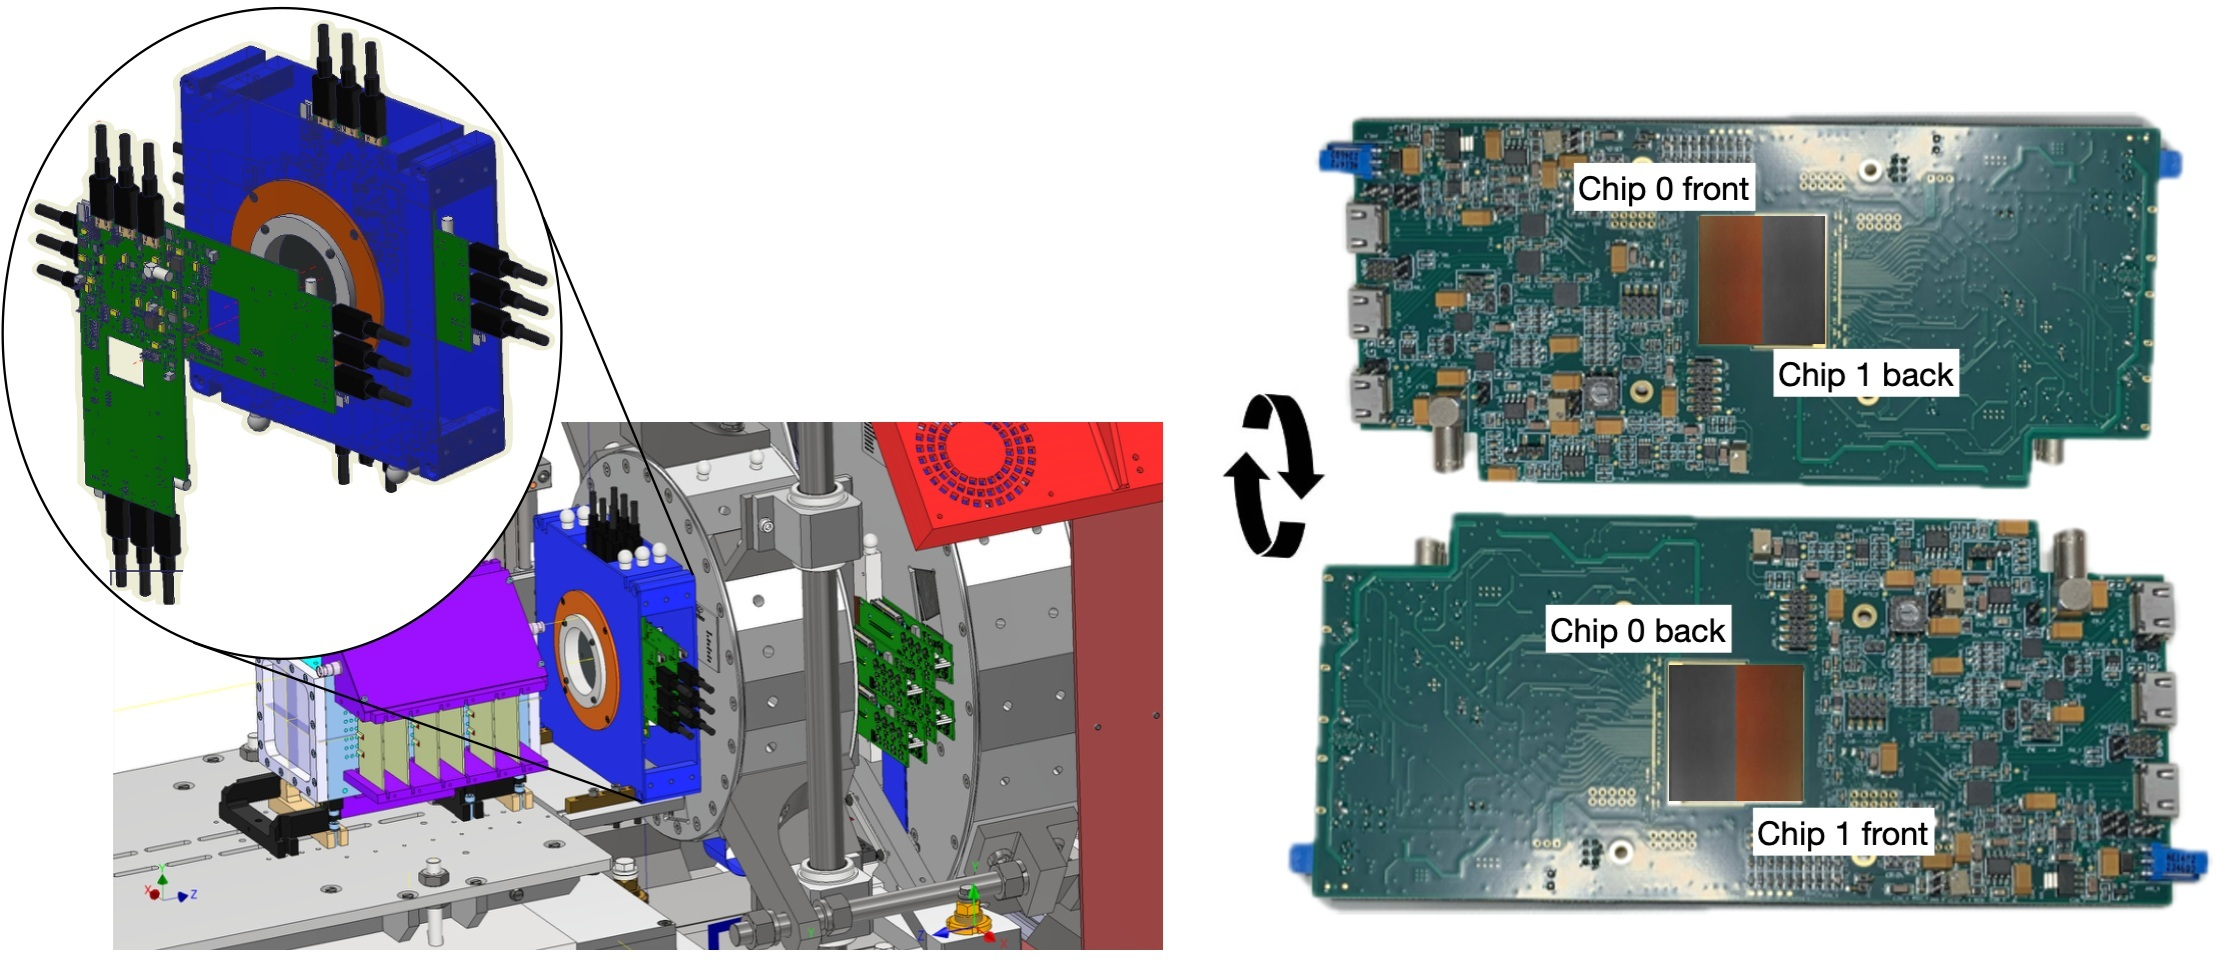
\includegraphics[width=0.98\linewidth]{new_vt_detector.jpg}
	\caption[The new MIMOSIS-2.1 Vertex Tracker]{On the left, schematic representation of the final configuration of the new MIMOSIS-2.1 VT. The zoom shows the orthogonal orientation of the $4$ proximity boards. On the right, front and back pictures of a single proximity board, with the chips bonded on it. From \cite{Rabaglia_2026}.}
	\label{fig:new_vt_detector}
\end{figure}
To fully support the superior timing performances of the MIMOSIS-2.1, the FOOT Collaboration has implemented a new dedicated Trigger and Data AcQuisition (TDAQ) system. After a brief description of the new VT TDAQ architecture, the following sections will focus on the VT trigger (see \autoref{sec:trigger_box}), being the module I mainly contributed to during my thesis.

\autoref{fig:trg_box_mimosis_daq} illustrates the main components of the VT TDAQ architecture, composed of all the boards, wires and connectors managing the data flow and the trigger/busy conditions. To understand the TDAQ system operation, let us follow the chronological data flow, supported by the help of \autoref{fig:trg_box_mimosis_daq}. First, when a charged particle passes through a single MIMOSIS-2.1 sensor, the hit data are transferred via HDMI differential signaling to the $2$ custom-developed DAQ boards in \autoref{fig:trg_box_mimosis_daq} (top left). Successively, the DAQ boards convert the signals into the single-ended standard, before transmitting them to the ``DAQ'' DE10-Nano board displayed in \autoref{fig:trg_box_mimosis_daq} (top left), which houses a Intel/Altera System-on-Chip (SoC) FPGA (Cyclone V) with a dual-core Cortex-A9 CPU. This DE10-Nano fulfills several duties: it generates the clock signal for the PB, handles the PB-chip communication via the I${}^2$C protocol and, most importantly, deserializes the received data before temporarily storing it on a DDR3 SDRAM. Once stored, the data signals wait for an external trigger, which is provided by the custom-designed DE10-Nano trigger board (hereafter referred to as Trigger Box or TrgBox) in \autoref{fig:trg_box_mimosis_daq} (right). The TrgBox collects the trigger signals raised by the WaveDAQ system (see the FOOT triggers in \autoref{sssec:tdaq_foot}) and distributes it to the DAQ boards via LVDS standard. After accepting the trigger signal, the DAQ DE10-Nano board opens a readout window centered on the trigger time, encompassing all the data frames and the respective metadata that will be sent to the FOOT central DAQ. The central DAQ finally recomposes the data fragments coming from each subdetector to assemble a full event, whose structure is displayed in \autoref{fig:data_fragment}.
\begin{figure}[H]
	\centering
	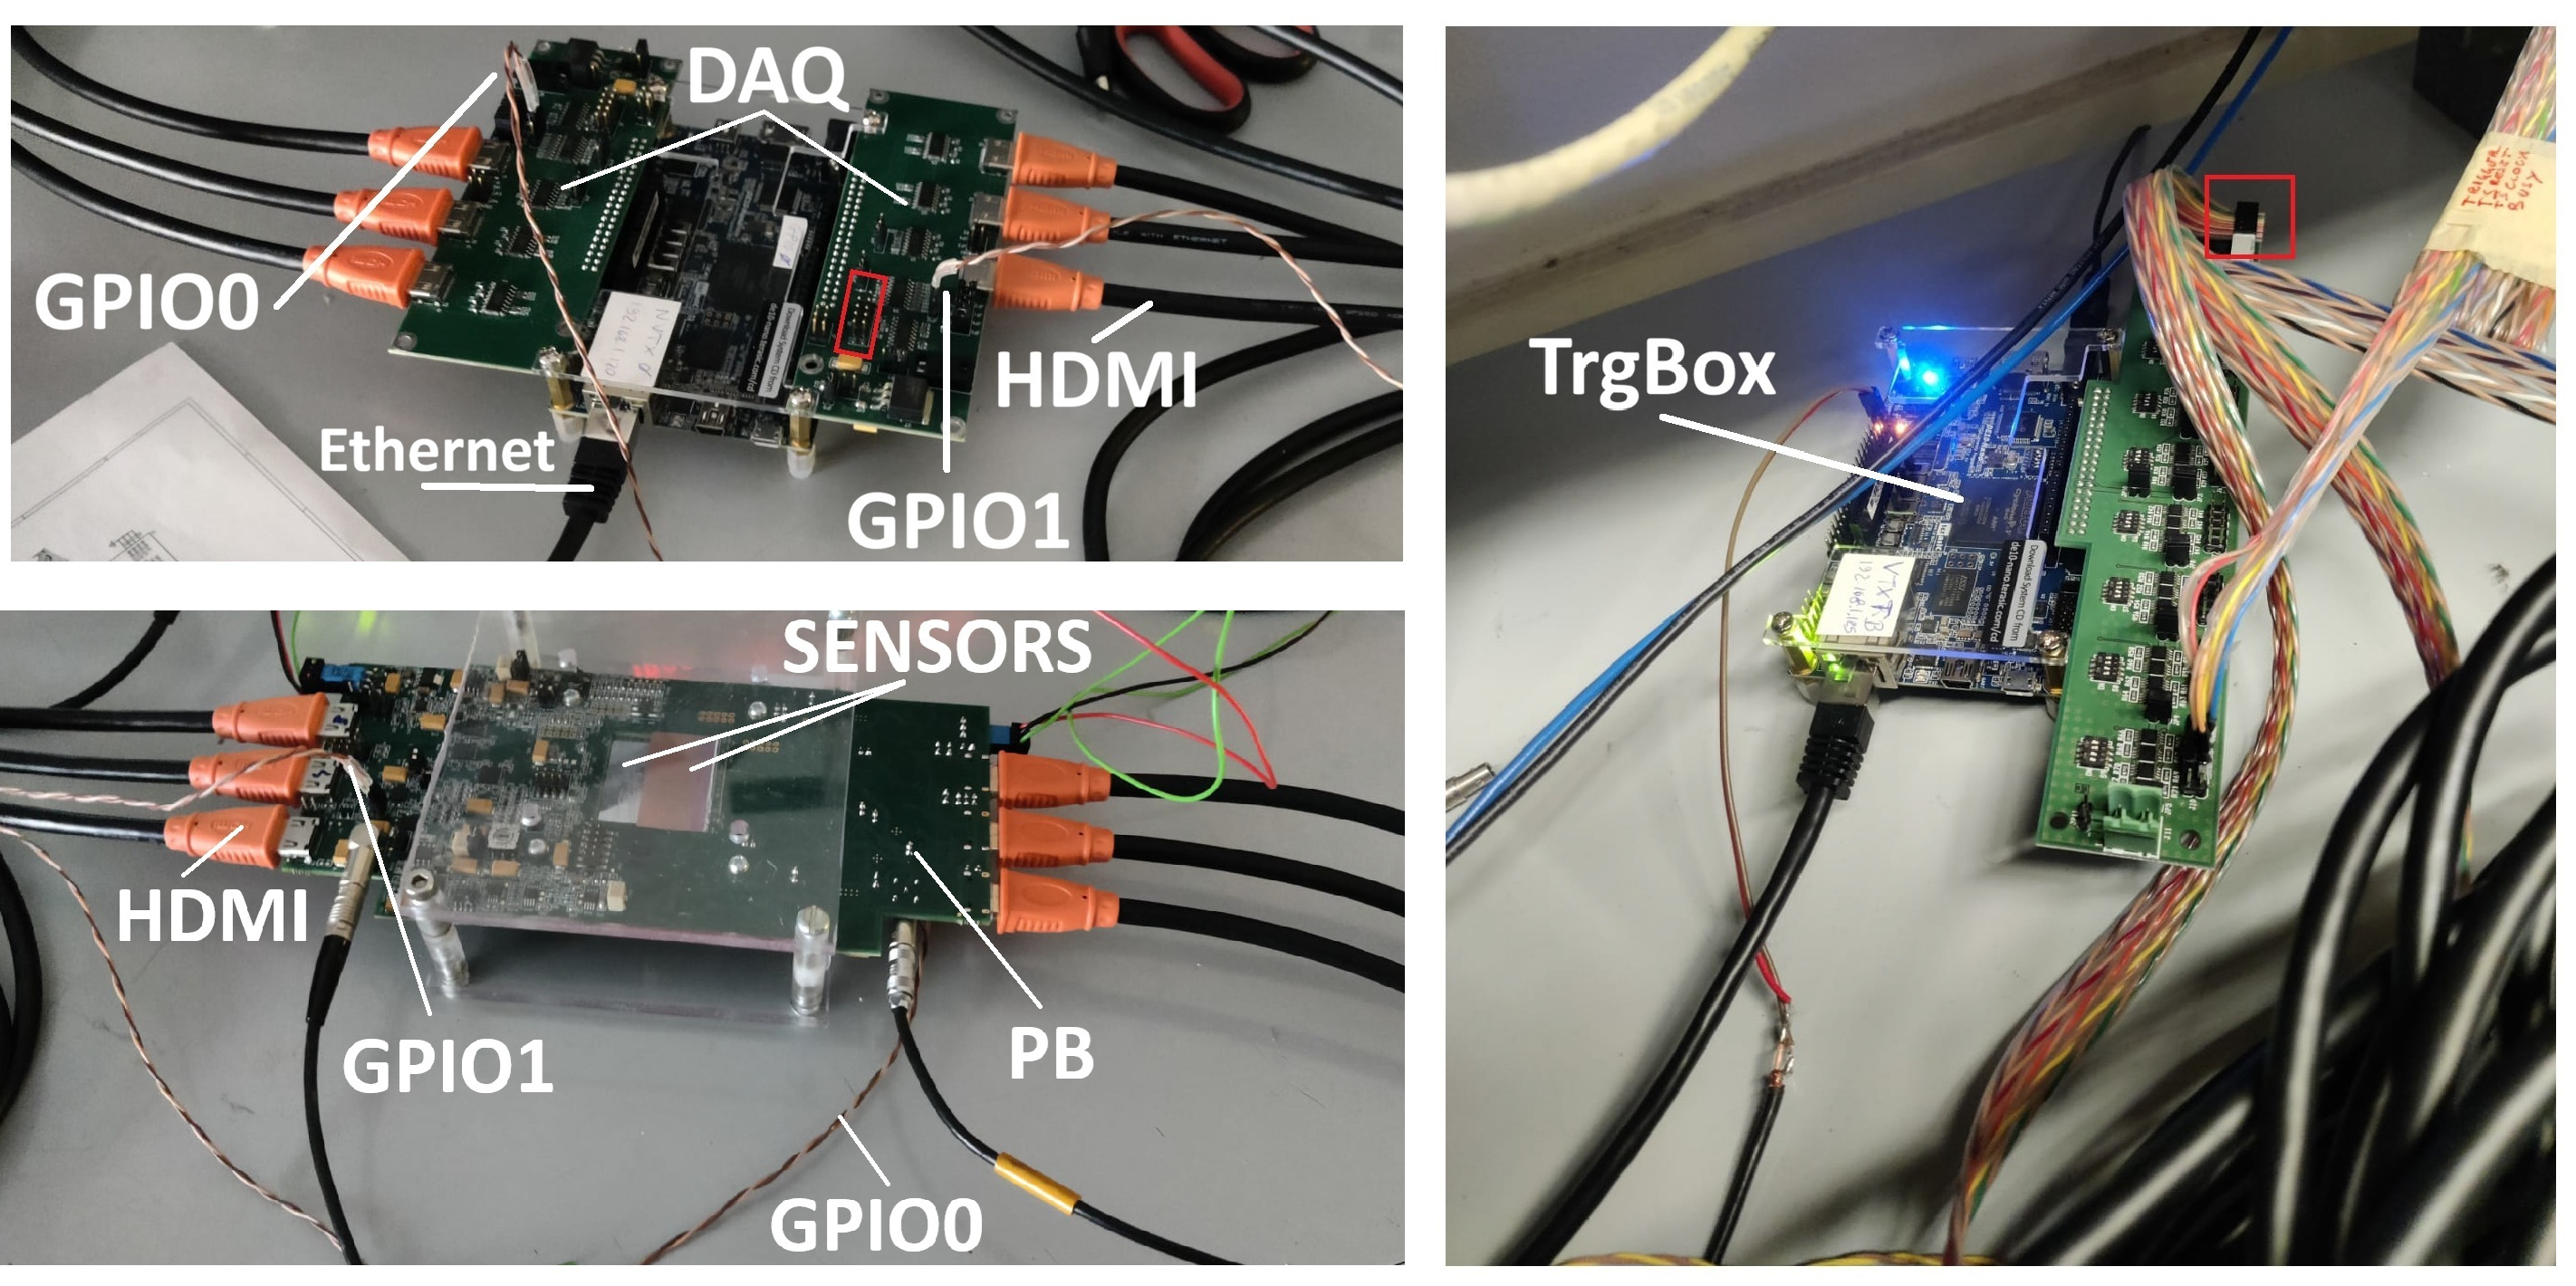
\includegraphics[width=0.98\linewidth]{trg_box_mimosis_daq.jpg}
	\caption[The new MIMOSIS-2.1 experimental setup]{Components of the experimental setup employed to test $1$ plane of the new VT. On the top left, DE10-Nano board coupled with two DAQ boards aimed at controlling the PB hosting the MIMOSIS-2.1 sensors with GPIO cables. $6$ HDMI connectors handle the data flow from the sensors. The picture also shows $2$ LEMO and $2$ clock cables, and $2$ power supply connectors. On the bottom left, PB and MIMOSIS-2.1 chips. On the right, TrgBox connected to the DAQ boards via twisted-pair LVDS ribbon cables. The tiny red boxes on the top left and on the right label the two ends of the ribbon cables used for the DAQ-TrgBox communication. Adapted from \cite{Rabaglia2025RoadToBTF}.}
	\label{fig:trg_box_mimosis_daq}
\end{figure}
\begin{figure}
	\centering
	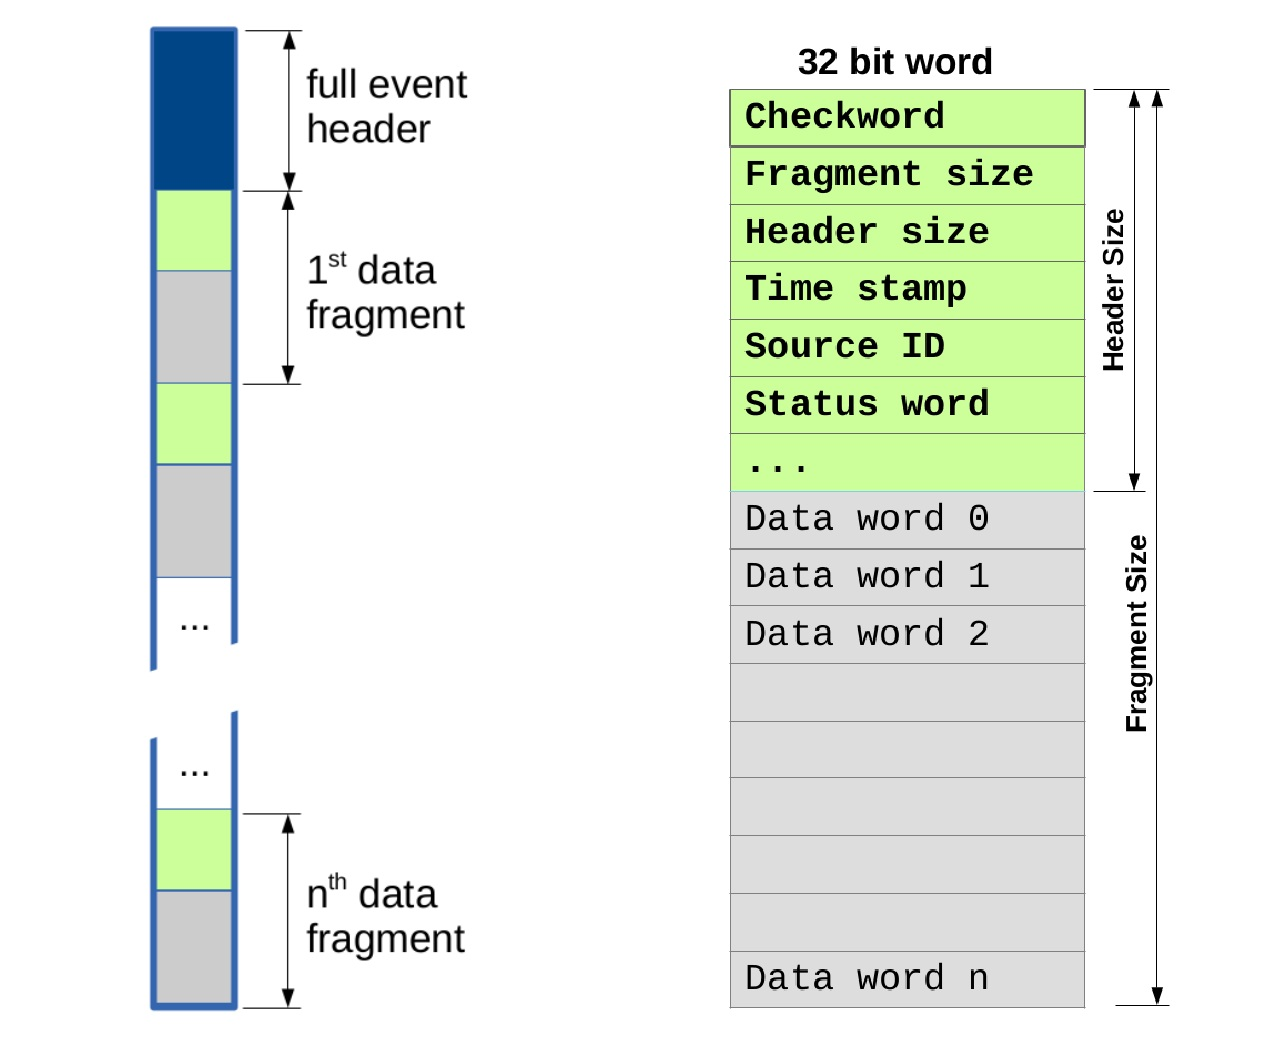
\includegraphics[width=0.98\linewidth]{data_fragment.jpg}
	\caption[Raw experimental data stream]{On the left, composition of a full event, consisting of a full event header and data fragments. On the right, a single data fragment and its payload, with header and data words. Each data word is made of $4\,\mathrm{bytes}$. From \cite{UbaldiPhDThesis}.}
	\label{fig:data_fragment}
\end{figure}
\section{Trigger Box}\label{sec:trigger_box}
As explained in \autoref{sec:new_vertex_tracker}, the data extrapolation from the new VT MIMOSIS-2.1 sensors foresees a dedicated trigger board (see the TrgBox in \autoref{fig:trg_box_mimosis_daq} (right)), which is thoroughly described in this section. The TrgBox consists of a Terasic DE10-Nano board system housing an Intel/Altera System-on-Chip (SoC) FPGA (Cyclone V) with a dual-core ARM Cortex-A9 CPU processor. \autoref{fig:de10-nano} shows a photograph of the top and bottom views of the board, with the relevant connectors and the key components.
\begin{figure}[H]
	\centering
	\begin{subfigure}[b]{0.49\linewidth}
		\centering
		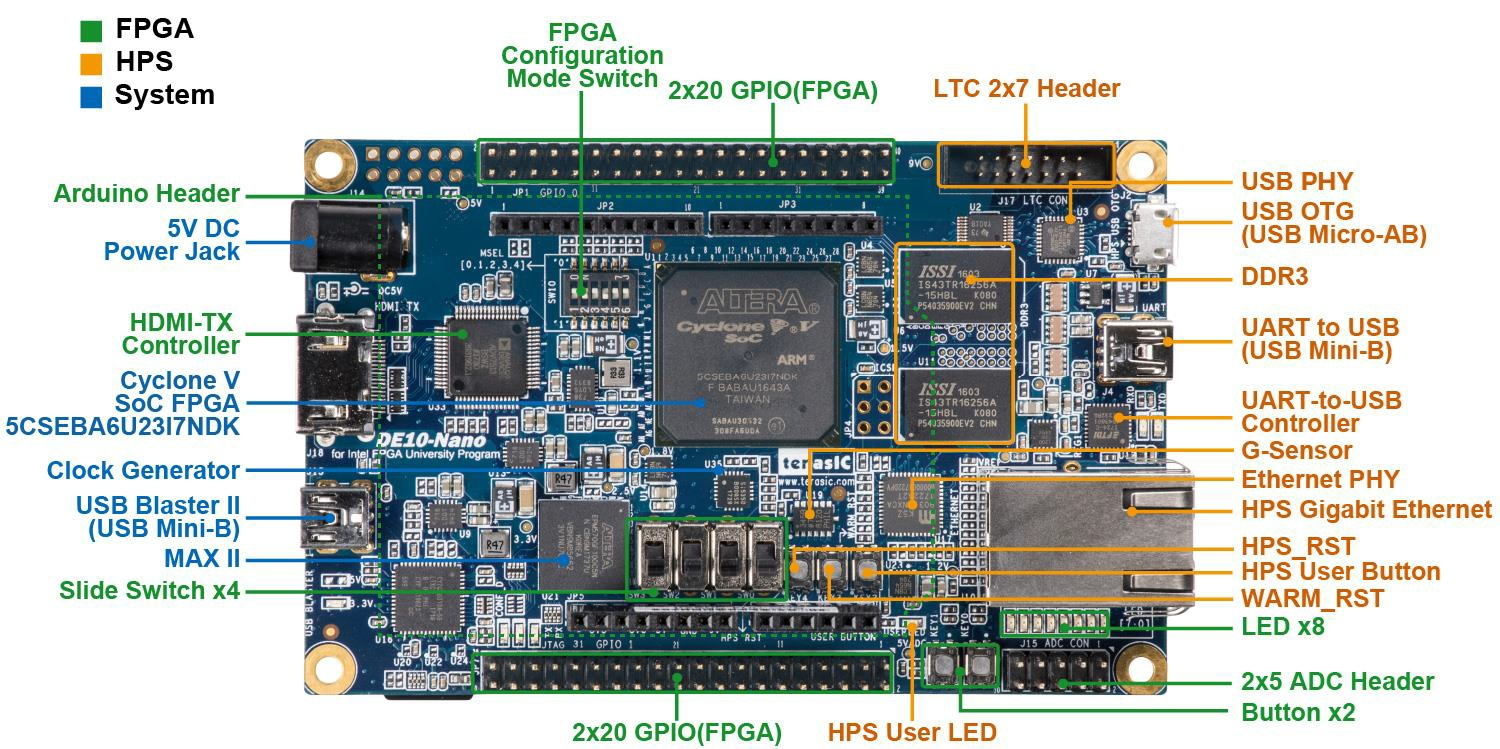
\includegraphics[width=0.7\linewidth]{de10-nano_top.jpg}
		\caption{Top view.}
		\label{fig:de10-nano_top}
	\end{subfigure}
	\hfill
	\begin{subfigure}[b]{0.49\linewidth}
		\centering
		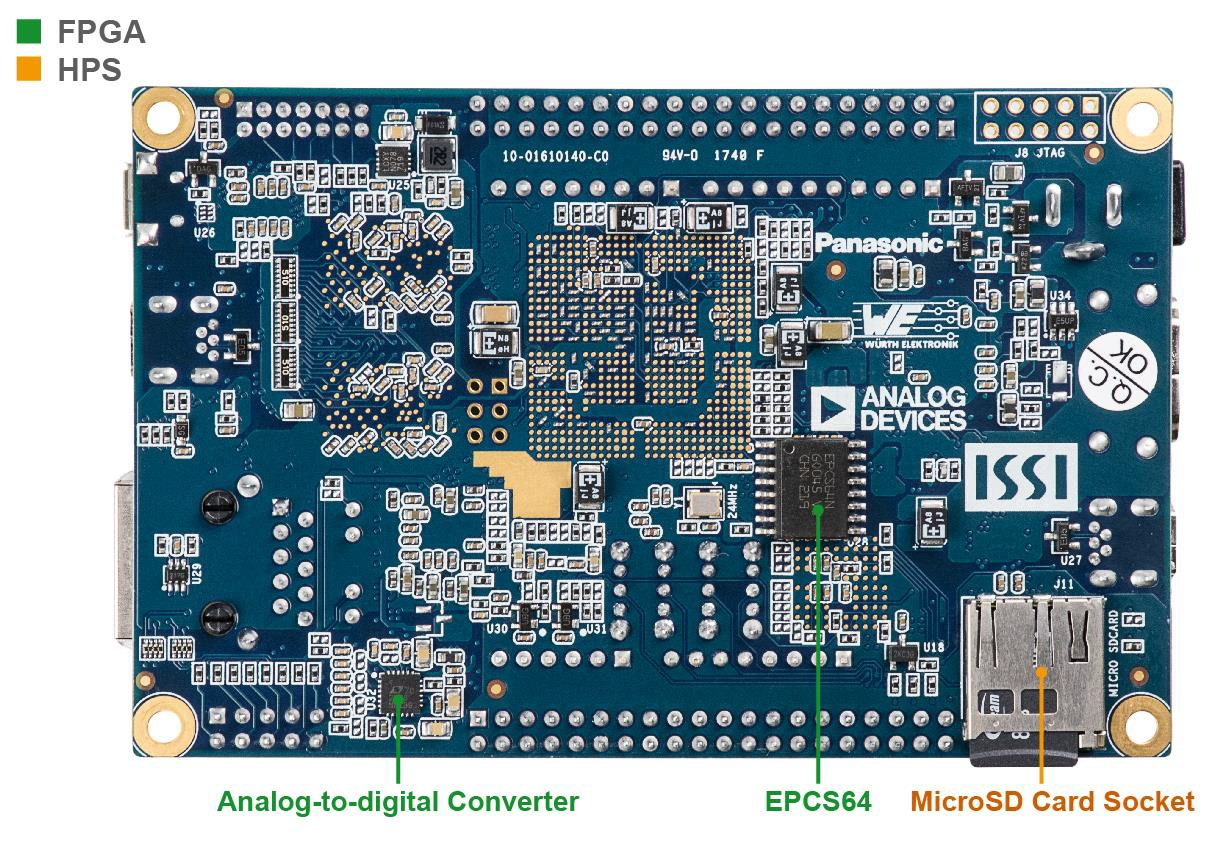
\includegraphics[width=\linewidth]{de10-nano_bottom.jpg}
		\caption{Bottom view.}
		\label{fig:de10-nano_bottom}
	\end{subfigure}
	\caption[Terasic DE10-Nano board]{Top and bottom views of the Terasic DE10-Nano board, with its relevant connectors and components. From \cite{terasic_de10_nano_board}.}
	\label{fig:de10-nano}
\end{figure}















%Time synchronization across all detector subsystems represents a critical aspect of the TDAQ  design, given the high number and heterogeneity of involved detectors. The V2495 trigger board  continuously generates a 1 MHz Timestamp Clock (TS clock) distributed to all detectors, which is  sampled and recorded in the event payload. This redundant timing information is essential for online  monitoring of alignment, allowing also to perform offline synchronization of  acquired data in case of temporary issues on trigger distribution. The busy logic, also managed  centrally by the trigger board, implements a logical OR of all detector busy signals: if any 
%detector reports a busy condition, trigger generation is inhibited until all subsystems are ready  to acquire. This mechanism, combined with backpressure propagation through the many buffers  spread throughout the acquisition system, guarantees data integrity preventing buffer overflows and  subsequent data losses.

% properly process the event and to allow detectors to get ready for the next event.
%All busy signals, in addition to trigger, in the FOOT experiment are managed by
%the central trigger board, i.e. the CAEN V2495 board, a general purpose programmable
%FPGA and I/O unit hosted in the VME crate. The board receives busy signals from all
%the detectors and performs their logic OR: if at least one detector is not ready to take
%data, no trigger will be issued even if generated by the WaveDAQ. The busy time length
%can vary from event to event even if most of FOOT detectors have it fixed (excluding
%variable timing to empty buffers): as already said, the slowest detector is the Vertex
%detector


% patch panel to distribute signals with
%the possibility to forward some copies of candidate trigger signals from the Wavedream
%system without waiting for V2495 board. In this way it is possible to avoid the jitter
%introduced by the sampling rate of the trigger board







%Detectors can be triggered or triggerless: in the former case, detector are read only
%when a trigger occurs while in the latter the data flux from detectors is continuous.
%Among FOOT detectors, only the Vertex sensors (M28 chips) have a triggerless architecture:
%however, the Vertex readout electronics sends data to the central DAQ only if
%a trigger is received




%Caro Pasquini,
%
%provo a rispondere in linea:
%
%Il 10/12/2025 11:14, Simone Pasquini - simone.pasquini7@studio.unibo.it ha scritto:
%Rimango in attesa di sue indicazioni in merito agli sviluppi software/hardware della trgBox.
%per questioni di debug è opportuno avere un data channel anche per la trigger box. La cosa è relativamente semplice, visto che si tratta di leggere i registri da 28 a 34 e metterli in uno stream dati. Praticamente si tratta di aggiornare un file sorgente che è il SOCServerInterface.cpp, metodi readData e wordsAvailable. E' facile da fare e se vuole glielo lascio fare.
%
%Per ciò che concerne la documentazione, se non erro la scorsa volta si parlava di redigere uno scritto contenente informazioni sui registri della trgBox. Tale documento deve:
%essere esaustivo o sintetico?
%avere un formato particolare?
%Lo scritto deve essere sintetico. Sarà un po' sulla base del "ProgettoTriggerBox.mb", con appena più ufficialità.
%
%Il 09/12/2025 09:00, Simone Pasquini - simone.pasquini7@studio.unibo.it ha scritto:
%come concordato, le invio in allegato un file .zip con all'interno:
%Il file .rbf, che include:
%le modifiche effettuate la scorsa volta
%Il BusyTime.vhd aggiornato con il reset del contatore all'arrivo di un nuovo segnale di Trigger
%La cartella bin/ aggiornata
%Il file script load.sh, che se vuole può utilizzare per caricare  file .rbf e cartella bin/ nella VTXBox eseguendo: ./load.sh DE10nano_TriggerBOX_DE250008.rbf bin/
%Intanto grazie per questo aggiornamento! Come avrà avuto modo di vedere dai mail che sono circolati, la stiamo usando con profitto.
%
%Inoltre, visto che la scorsa volta avevamo trovato incongruenze nei Monitoring registers 3 e 14 (relativi ai timeStamp + FIFO), ho voluto ripassare il TimeStampGenerator.vhd, al cui interno si genera il segnale di internal timeStamp con un periodo di 1 microsecondo, diverso dal periodo di 20 ns del segnale di Clock. Tale differenza non dovrebbe causare le problematiche osservate la scorsa volta, ma mi chiedevo se ci fosse un motivo particolare per cui al momento utilizziamo periodi differenti.
%Il Time Stamp dovrebbe essere univoco nell'intero esperimento. Nella funzionalità di Trigger Box "stand-alone" usiamo il time stamp interno, nella modalità di lavoro finale usiamo il Time Stamp generato all'esterno dalla scheda V2495. 
%
%In attesa di un suo riscontro (anche in merito alla gestione della FIFO), la ringrazio in anticipo per la sua disponibilità.
%Sulle fifo, le mando in allegato la documentazione di come si creano delle fifo con quartus. Per semplificare al massimo, le dico che la fifo che è usata per le informazioni di trigger è una fifo Single-Clock di tipo Show-Ahead. Quartus genera queste fifo con un segnale chiamato "rdreq" (read-request) è in realtà un "read-acknowledge". Si veda paragrafo 1.8. Caratteristica di questa fifo è che è lenta, cioè tra una lettura e la successiva occorrono sempre 2 colpi di clock (vedi anche figura 6 dell'allegato).
%
%Quando le sarà possibile, le chiedo gentilmente di farmi sapere se posso essere d'aiuto per quanto sopra riportato.
%In questi giorni siamo sempre in laboratorio a migliorare giorno per giorno il sistema. Se/quando passa, qualcosa da fare o da verificare sulla trigger box lo troveremo facilmente.
%
%A presto,
%
%Mauro Villa
%
%
%
%
%
%Da: Mauro Villa <mauro.villa@unibo.it>
%Inviato: mercoledì, dicembre 10, 2025 8:28:15 AM
%A: Sara Valentinetti <sara.valentinetti@bo.infn.it>; Simone Pasquini - simone.pasquini7@studio.unibo.it <simone.pasquini7@studio.unibo.it>; Sara Rabaglia <sara.rabaglia2@unibo.it>; Riccardo Ridolfi <Riccardo.Ridolfi@bo.infn.it>
%Oggetto: Info daq mimosis
%
%Carissimi tutti,
%
%vi aggiorno cumulativamente su alcuni sviluppi della DAQ Mimosis:
%
%- ieri siamo riusciti a far funzionare bene insieme la board con i due
%mimosis, la trigger box e la DAQ generale. Abbiamo acquisito dati che
%appaiono sensati (senza eventi vuoti) con un rate fino a 1 kHz. Ottimo!!
%Il run si chiude anche bene!!
%
%- per raggiungere questo risultato abbiamo dovuto fare qualche
%cambiamento minimale sul lato TDAQ generale e configurare bene i vari
%dispositivi.
%
%- Fino a prova contraria, congelerei i due firmware così come sono
%(versione 08 sulla triggerbox e 04 sulla nvtx0) e suggerirei di andare
%avanti sullo sviluppo della TDAQ generale e dell'hardware.
%
%Mi sono convinto che è meglio per il test alla BTF avere un data channel
%anche della trigger box. I cambiamenti da fare sono minimali (e sono
%soprattutto sul software della triggerbox), ma potrebbero essere
%importanti per il debug quando il sistema avrà N schede. Tra i lavori
%che ci sono da fare segnalo (in ordine random):
%
%- documentare hardware, software e configurazioni
%
%- inserire un modulo con gnam
%
%- fare misure con sorgente
%
%- lavorare con 2 schede e prepararsi al salto con N>2 schede.
%
%- preparare l'hardware per un run di cosmici natalizi....
%
%Oggi alle 12 arriva la sorgente.
%
%A presto,
%
%Mauro



\chapter{Experimental part}
% Here you will have to justify the use of 200 Mev/u carbon-carbon interactions. You can mention what you have said for the PhD application but also that FOOT has covered up to now a limited set of beam-target-energy configurations (and then you have to check page 2 of this article https://journals.aps.org/prc/pdf/10.1103/17nq-3ddt) when it states some key measurements have been performed already [16–25] (which includes the FOOT experiment publication)

\section{Global analysis with SHOE}\label{sec:shoe} % if this changes, change also the ref in chapter 2
	
	\chapter*{Acknowledgement}
\addcontentsline{toc}{chapter}{Acknowledgement}

	\appendix
\renewcommand{\chaptermark}[1]{%
	\markboth{\MakeUppercase{APPENDIX\ \thechapter\ --\ #1}}{}
}
\chapter{Radiobiological aspects of ionizing radiations}\label{ch:radiobiology}
The aim of this chapter is to provide an overview of the most important biological effects induced by ionizing radiation and to define the physics parameters employed in the contexts of radiobiology, dosimetry and medical physics.
\section{Biological damages of ionizing radiation}\label{sec:biological_damages_ionizing_radiation}
Both the conventional radiotherapy (which uses X-rays, i.e., photons) and the more advanced Particle Therapy (PT) take advantage of the ionizing radiation to damage the cancerous tissues of a patient, triggering the death of the diseased cells which they consist of. The ionizing radiation produces various effects on biological tissues, which largely depend on the beam composition, its energy and the properties of the irradiated tissues. To beat cancer, it is not necessary to eliminate all the cancerous cells, but it is sufficient to impede their indefinite reproduction through a reproductive cell death. To achieve this goal, ionizing radiation need to kill the cell DNA by means of either direct or indirect damage. Direct damage is the most uncommon one, as the DNA occupies only $2$--$3\%$ of the total cell volume. Direct damage can be divided into Single Strand Breaks (SSB) and Double Strand Breaks (DSB): in SSBs, a break occurs in only one nucleotide strand of the DNA double helix, whereas in DSBs both nucleotide strands are damaged. Both SSB and DSB are illustrated in \autoref{fig:dna_damages}.
\begin{figure}[H]
	\centering
	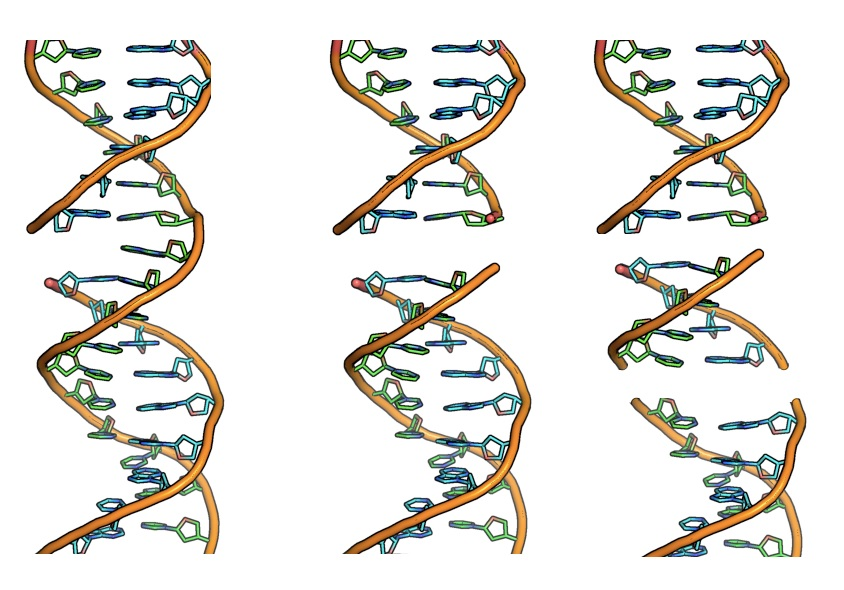
\includegraphics[width=0.98\linewidth]{danni_dna.jpg}
	\caption[Tracking region]{Schematic representation of SSBs (left), DSBs (center), and clusters of DSBs (right). From \cite{unipv_conference}.}
	\label{fig:dna_damages}
\end{figure}
Indirect damage occurs when the ionizing radiation does not hit the DNA directly, but rather the neighboring cell elements. As water makes $\gtrsim70\%$ of the total cell mass \cite{cooper2000cell}, the ionizing radiation often hits water, leading to the release of free radicals. Free radicals are neutral atoms or molecules possessing one unpaired electron in the outermost orbital, a feature which makes them highly unstable and reactive. The chain of chemical reactions (summarized below) which lead to the formation of free radicals is called radiolysis of water. The byproducts of radiolysis consists of electrons, atoms, molecules, and ions which, by diffusing, indirectly damage DNA, leading to cell death. The ionization of a water molecule \ce{H2O} is given by:
\begin{equation}
	\ce{H2O ->[Ionizing radiation] H2O^{+} + e^-},
	\label{eq:radiolisi1}
\end{equation}
from which a positive ion \ce{H2O^{+}} and an electron \ce{e^-} are produced. After a certain time interval, some traveling electrons lose a significant part of their kinetic energy and are captured by another water molecule, resulting in the formation of a negative ion \ce{H2O^{-}}:
\begin{equation}
	\ce{H2O + e^{-} ->[Electron capture] H2O^{-}}.
	\label{eq:radiolisi2}
\end{equation}
Subsequently, the products of \autoref{eq:radiolisi1} and \autoref{eq:radiolisi2} dissociate as follows:
\begin{subequations}
	\begin{align}
		\label{eq:dissociazione1}
		\ce{H2O^{+} ->[Dissociation] H^{+} + OH^{.}}\\
		\label{eq:dissociazione2}
		\ce{H2O^{-} ->[Dissociation] OH^{-} + H^{.}},
	\end{align}
\end{subequations}
whose products are the hydrogen \ce{H^{+}} and the hydroxide \ce{OH^{-}} ions, along with the hydroxyl \ce{OH^{.}} and the hydrogen \ce{H^{.}} free radicals. Among the various chemical reactions that can subsequently occur (whose reactants are the products of \autoref{eq:dissociazione1} and \autoref{eq:dissociazione2}), the following are reported:
\begin{subequations}
	\begin{align}
		\label{eq:prodotto1}
		\ce{H^{.} + OH^{.} &-> H2O}\\
		\label{eq:prodotto2}
		\ce{H^{+} + OH^{-} &-> H2O}\\
		\label{eq:prodotto3}
		\ce{2OH^{.} &-> H2O2}.
	\end{align}
\end{subequations}
Clearly, \autoref{eq:prodotto1} and \autoref{eq:prodotto2} are harmless reactions (they generate water molecules), whereas \autoref{eq:prodotto3} leads to the formation of hydrogen peroxide \ce{H2O2}, a substance that highly harmful to the cell. Indeed, \ce{H2O2} is capable of altering the structure and function of proteins, mutating nucleotide bases and generating SSBs in DNA \cite{ros}. Generally, \ce{H2O2} and other oxygen-related chemical species (such as the two radicals superoxide anion \ce{O2^{-.}} and hydroxyl \ce{OH^{.}}) are grouped in the wider ROS (Reactive Oxygen Species) family, whose elements can all lead to the reproductive cell death.
\section{Dosimetric quantities}\label{sec:dosimetric_quantities}
In radiobiology, the branch of dosimetry is fundamental to define and quantify the physical quantities that describe the irradiation of matter and the consequent biological effects. Dosimetric studies are particularly important at the treatment planning stage, as they allow to assess the correct balance between the damaging irradiation of the tumor and the risks of toxicity to healthy organs. One of the aims of the International Commission on Radiation Units and Measurements (ICRU) is to define the physics parameters used in dosimetry, some of which are reported in the following.
\subsection{Absorbed, equivalent and effective dose}\label{ssec:dose_definition}
First and foremost, the basis quantity in dosimetry is the particle fluence $\phi$, defined as the number of particles $dN$ (for example, the protons within a beam) passing through an unit area $dA$ perpendicular to the beam direction. The fluence can be expressed in its differential form as follows:
\begin{equation}
	\phi=\frac{dN}{dA}
	\label{eq:fluence}.
\end{equation}
Using the particle fluence, it is possible to define the absorbed dose $D$ as the energy $dE$ absorbed by an irradiated material of unit mass $dm$:
\begin{equation}
	D=\frac{dE}{dm}=\frac{\left(dE/dx\right)\Delta x N}{\rho \Delta x A}=\phi\frac{\left(dE/dx\right)}{\rho},
	\label{eq:dose_as}
\end{equation}
where $dE/dx$ is the stopping power defined in \autoref{eq:bethe_bloch}, $N$ is the number of particles in the beam and $\rho$ is the volumetric mass density of the irradiated material (obtained from its cross-sectional area $A$ and its thickness $\Delta x$, which is parallel to the beam direction). According to the International System of Units (SI), the unit of measurement of the absorbed dose $D$ is the Gray (Gy), and represents the amount of radiative energy received by the patient during therapy divided by the mass of the irradiated tissue.

Generally, when two tissues absorb the same dose, the subsequent biological effects may be different. This is connected to the fact that the biological damage varies depending on the type and energy of the absorbed radiation as well as on repair mechanisms activated by the irradiated tissue after treatment. In radiotherapy, the local biological effects can be described by several quantities, namely the LET (see ?? let), the RBE (see ?? rbe) and the OER (see ?? OER). Due to the inherent complexities of these quantities, everyday radiation protection uses a simpler way to asses the biological effectiveness of a given radiation, which is based on the concept of equivalent dose $H$:
\begin{equation}
	H=\sum_{R}w_RD_{R},
	\label{eq:dose_eq}
\end{equation}
where $D_{R}$ is the absorbed dose relative to the $R$-th radiation (measured in Sievert (Sv) in the SI) and $w_R$ weights the hazard of the $R$-th radiation. $w_R$ is a dimensionless weighting factor given by the ratio between the biological damage produced by the absorption of $1\,\mathrm{Gy}$ of radiation $R$ and the biological damage produced by $1\,\mathrm{Gy}$ of $\gamma$ rays. $H$ is still an incomplete quantity, as it does not quantify biological effects in relation to the type of organ or tissue irradiated. For this reason, the effective dose $E$ is defined (always measured in Sievert), which includes the biological effects due to the type of radiation $R$ and to the specific response of the irradiated tissue $T$:
\begin{equation}
	E=\sum_{T}w_TH=\sum_{T}w_T\sum_{R}w_RD_{R},
	\label{eq:dose_eff}
\end{equation}
where $w_T$ is a weighting factor for the $T$-th tissue such that $\sum_{T}w_T=1$, where the sum runs over all tissues of the human body. $w_T$ is larger for tissues that are more sensitive to radiation: they respond better to the treatment, but they are also more prone to develop radiation-induced cancer.
\subsection{Linear energy transfer}\label{ssec:let}
The Linear Energy Transfer (LET) of a ionizing radiation is the amount of energy $dE$ transferred to the irradiated material per unit length of the track $dx$:
\begin{equation}
	\text{LET}=\frac{dE_\Delta}{dx}.
	\label{eq:let}
\end{equation}
Although the LET has a very similar definition to the stopping power $dE/dx$ defined in \autoref{eq:bethe_bloch}, they are not quite the same quantity. Indeed, the stopping power is related to the energy lost by the particle beam in the medium it crosses (per unit distance), LET refers to the energy absorbed by the medium (per unit distance). In addition, in \autoref{eq:let} a $\Delta$ appears because the definition of LET takes into account only the small energy transfers close to the particle's trajectory, excluding the more energetic ionizations from long-range $\delta$ electrons (whose energy is greater than a threshold $\Delta$). In the mathematical limit $\Delta\rightarrow+\infty$, there would no longer be electrons with $E>\Delta$, meaning that the stopping power and LET would be equivalent quantities. These considerations allow us to derive the relation linking the stopping power and LET:
\begin{equation}
	\text{LET}=\frac{dE_\Delta}{dx}-K_{E>\Delta},
	\label{eq:let&stoppingpower}
\end{equation}
where $K_{E>\Delta}$ is the kinetic energy of electrons with energy $E>\Delta$.

The LET value is inherently connected to particles' ionization density: high-LET radiations are densely ionizing, while low-LET radiations produce sparse ionization events, as illustrated in \autoref{fig:ioniz_density}. As they generate more frequent and clustered ionization events, higher-LET radiations cause greater biological damage to tissues, as schematized in \autoref{fig:damage_let}. \autoref{fig:damage_let} shows that low-LET radiations, such as X-rays or $\gamma$ rays, mainly induce isolated DNA damage leading to SSBs, while high-LET radiations, including $\alpha$ particles or heavy ions, generate more destructive DNA damage, resulting in DSBs \cite{Roobol2020-fp}.
\begin{figure}[H]
	\centering
	\begin{subfigure}[b]{0.48\linewidth}
		\centering
		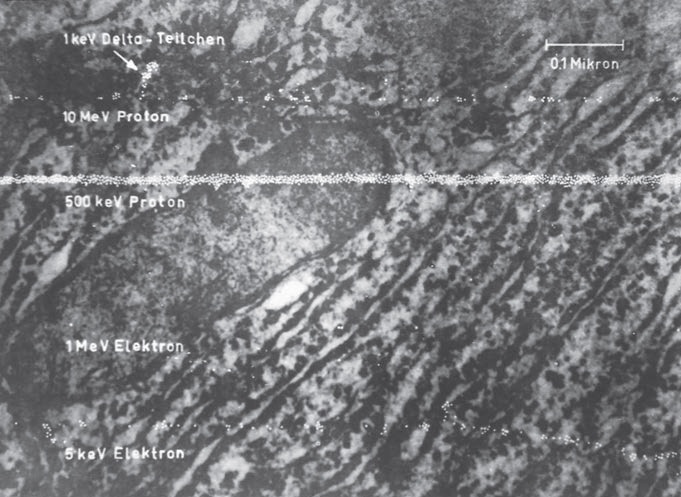
\includegraphics[width=0.8\linewidth]{ioniz_density.jpg}
		\caption{Variation of ionization density associated with different types of radiation. From \cite{hall2012radiobiology}.}
		\label{fig:ioniz_density}
	\end{subfigure}
	\hfill
	\begin{subfigure}[b]{0.48\linewidth}
		\centering
		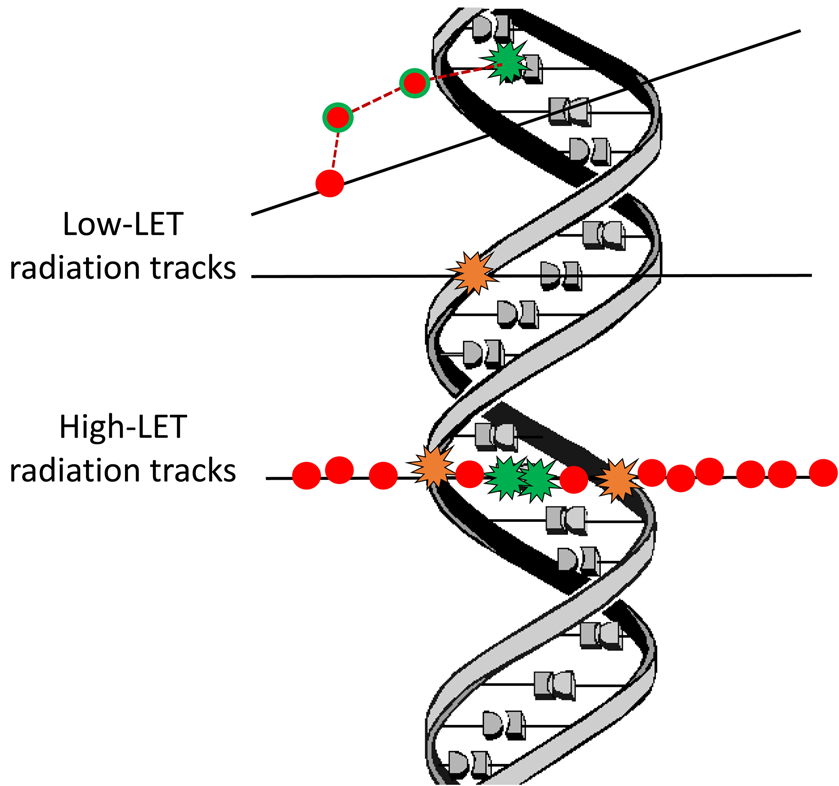
\includegraphics[width=\linewidth]{damage_let.png}
		\caption{Typical DNA damage caused by low-LET radiation (top) and high-LET radiation (bottom). From \cite{Fabbrizi_Parsons_2022}.}
		\label{fig:let}
	\end{subfigure}
	\caption[Ionization density and LET]{How different values of LET lead to diverse ionization densities and biological consequences.}
	\label{fig:damage_let}
\end{figure}
From \autoref{fig:proton_carbon_let}, it can be viewed that the LET values of protons and carbons rise with the penetration depth, in accordance with the fact that the stopping power increases when particles slow down. On the other hand, in the entrance channel protons and carbon ions show discrepancies: the former cause damages every $90\,\mathrm{nm}$ (insufficient to hit the DNA double strand, whose diameter is $2\,\mathrm{nm}$), while carbons damage the DNA every $4\,\mathrm{nm}$ (sufficient to generate an SSB). Similarly, at the Bragg peak protons and carbon ions cause damage every $4\,\mathrm{nm}$ and every $0.3\,\mathrm{nm}$ (sufficient to generate SSBs and DSBs, respectively). Therefore, carbon ions are more damaging than protons near the Bragg maximum, but in the entrance channel they cause much more damage than protons. This difference must be taken into account during treatment planning in order to adapt the patient's characteristics to the beam properties.
\begin{figure}[H]
	\centering
	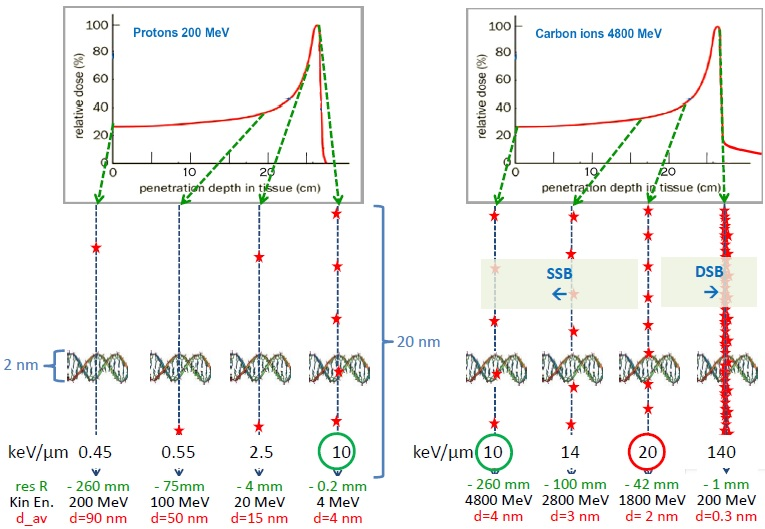
\includegraphics[width=0.9\linewidth]{proton_carbon_let.jpg}
	\caption[LET effects in protons and carbons]{Microscopic distribution of proton and carbon ionizations on a nm scale, along with the corresponding LET, depth reached, kinetic energy and average distance of damage creation \cite{slide_spighi}.}
	\label{fig:proton_carbon_let}
\end{figure}
\subsection{Relative biological effectiveness}\label{ssec:rbe}
The Relative Biological Effectiveness (RBE) of an ionizing radiation $R$ is a dimensionless number given by the ratio between the dose $D_\gamma$ released by $\gamma$ rays and the dose $D_R$ released by a given radiation $R$ needed to achieve the same biological effect, for a fixed cell survival rate $S$:
\begin{equation}
	\text{RBE}=\frac{D^S_\gamma}{D^S_R}.
	\label{eq:rbe}
\end{equation}
For example, if a radiation $R$ has $\text{RBE}>1$, this means that a smaller dose of $R$ is needed to achieve the same biological damage as $\gamma$ rays (in other words, radiation $R$ is more effective than $\gamma$ rays). Evaluating the RBE is rather complex, since it depends on the type of radiation and its energy, the LET (see \autoref{fig:let_rbe}), the cell type and its survival rate (see \autoref{fig:survival_dose}), the oxygenation status (see ?? OER sec) and whether fractionation is employed \cite{Choi2012-ef}. The \autoref{tab:rbe} reports some values of RBE for several radiations.



%for analytical formula of biological dose refer to https://iopscience.iop.org/article/10.1088/1367-2630/10/7/075003/pdf





\chapter{\texorpdfstring{$\chi^2$}{χ²} minimization method}\label{ch:chi_squared_min}
The $\chi^2$ minimization method is founded on the $\chi^2$ test, a probabilistic test that provides criteria for verifying the consistency of theoretical hypotheses with a set of experimental data. Specifically, the $\chi^2$ test is based on the evaluation of the $\chi^2$ function, reported in \autoref{eq:chi_square_method}, which expresses the discrepancy between theory and experimental data. This deviation is calculated using the sum of the squared differences between the measured values $y_k$ and the expected values $f\left(x_k;\alpha_j\right)$, and depends on the measurements $x_k$ and the parameters $\alpha_j$:
\begin{equation}
	\chi^2=\sum_{k=1}^N\left(\frac{y_k-f\left(x_k;\alpha_j\right)}{\sigma_k}\right)^2,
	\label{eq:chi_square_method}
\end{equation}
where $\sigma_k$ is the uncertainty associated with the $N$ measurements $y_k$ \cite{Fornasini2008}. The minimum $\chi^2$ method consists of deriving the parameters\footnote{From a mathematical point of view, the parameters are constraints on the minimization problem.} $\alpha_j$ to minimize the $\chi^2$ function in \autoref{eq:chi_square_method}.

Applying the $\chi^2$ minimization method on the three mass estimates given in \autoref{eq:a1}, \autoref{eq:a2} and \autoref{eq:a3}, the $\chi^2$ function becomes:
\begin{equation}
	\chi^2=\frac{\left(\text{ToF}-T\right)^2}{\sigma^2_{\text{ToF}}}+\frac{\left(p-P\right)^2}{\sigma^2_{p}}+\frac{\left(E_\text{kin}-K\right)^2}{\sigma^2_{E_\text{kin}}}+\transp{\vect{A}}\matr{B}\vect{A},
	\label{eq:chi_square}
\end{equation}
where $\text{ToF}$, $p$ and $E_\text{kin}$ are the physical quantities reconstructed using the FOOT electronic setup, $\sigma_{\text{ToF}}$, $\sigma_{p}$ and $\sigma_{E_\text{kin}}$ the relative uncertainties and $T$, $P$ and $K$ are three of the four minimization parameters. The \autoref{eq:chi_square} contains also the vector $\vect{A}$ (and its transposed $\transp{\vect{A}}$), given by the following expression:
\begin{equation}
	\vect{A}=
	\begin{pmatrix}
		A_1-A\\
		A_2-A \\
		A_3-A\\
	\end{pmatrix}
	,
	\label{eq:vector_A}
\end{equation}
where $A_1$, $A_2$ e $A_3$ are the experimental masses given by \autoref{eq:a1}, \autoref{eq:a2} and \autoref{eq:a3}, and $A$ is the fourth minimization parameter. The matrix $\matr{B}$ contains the uncertainties associated with $A_1$, $A_2$ and $A_3$ estimates, which, as already discussed, are not independent. Indeed, the correlation between the uncertainties of the mass number measurements is encompassed by the correlation matrix $\matr{C}$, which is related to $\matr{B}$ as follows:
\begin{equation}
	\matr{B}=\left(\matr{C}\transp{\matr{C}}\right)^{-1},
	\label{eq:B_funct_C}
\end{equation}
where, specifically, $\matr{C}$ entries are made explicit in \autoref{eq:correlation_matrix} \cite{foot_cdr,valle2019design}:
\begin{equation}
	\matr{C}=
	\begin{pmatrix}
		\frac{\partial A_1}{\partial T}dT&\frac{\partial A_1}{\partial P}dP&0\\
		\frac{\partial A_2}{\partial T}dT&0&\frac{\partial A_2}{\partial K}dK\\
		0&\frac{\partial A_3}{\partial P}dP&\frac{\partial A_3}{\partial K}dK\\
	\end{pmatrix}
	.
	\label{eq:correlation_matrix}
\end{equation}

If the parameters $\left(T,P,K,A\right)$ were thought of as variables of a four-dimensional space, the problem of minimizing $\chi^2$ is analogous to a problem of finding the minimum of a vector-valued function. Therefore, to obtain parameters $\left(T,P,K,A\right)$ that are the closest to the ``true'' parameter values, a minimization fit can be performed. The four-dimensional point where the $\chi^2$ assumes the minimum value will then correspond to the values of $\left(T,P,K,A\right)$ that are the closest to the ``true'' parameter values. A common strategy used to find minima within the ROOT framework is to employ Minuit \cite{JAMES1975343}, which performs multiple minimization steps to find a global $\chi^2$ minimum rather than a local minimum, ensuring that the final output parameters are sufficiently accurate.
\chapter{Augmented Lagrangian Method}\label{ch:alm_squared_min}
The Augmented Lagrangian Method (ALM) is an algorithm that addresses a constrained minimization problem of a multi-variable function $f\left(\vect{x}\right)$ by employing an unconstrained minimization problem in a larger parameter space. The ALM is a ``modified'' Lagrange multiplier method in which the minimization of the Lagrangian function $\mathcal{L}\left(\vect{x};\vect{\lambda}\right)$ with respect to the vector variable $\vect{x}$ is replaced by the minimization of an ``augmented'' Lagrangian $\mathcal{L}_{ALM}\left(\vect{x};\vect{\lambda},\mu\right)$ defined as:
\begin{equation}
	\begin{aligned} 
		\mathcal{L}_{ALM}\left(\vect{x};\vect{\lambda},\mu\right)&=\mathcal{L}\left(\vect{x};\vect{\lambda}\right)+\frac{1}{2\mu}\sum_{i=1}^{m}c_i^2\left(\vect{x}\right)=\\ 
		&=f\left(\vect{x}\right)+\sum_{i=1}^{m}\lambda_ic_i\left(\vect{x}\right)+\frac{1}{2\mu}\sum_{i=1}^{m}c_i^2\left(\vect{x}\right),
	\end{aligned}
	\label{eq:augmented_lagrangian_funct}
\end{equation}
where $f\left(\vect{x}\right)$ is the original function to be minimized, $\vect{\lambda}$ is the $m$-dimensional vector containing the Lagrange multipliers $\lambda_i$ associated with the $m$ constraints $c_i\left(\vect{x}\right)$ and $\mu$ is a positive parameter. The final summation term in \autoref{eq:augmented_lagrangian_funct} is usually referred to as the ``penalty term'', and it is a function of the problem constraints weighted with a penalty parameter $\mu$. If the $c_i\left(\vect{x}\right)$ are zero, the penalty term vanishes, while it is large if $c_i\ne0$ and $\mu\rightarrow0$.

In ALM, successive unconstrained minimizations of \autoref{eq:augmented_lagrangian_funct} are performed: starting from a solution $\left(\vect{x}^0,\vect{\lambda}^0\right)$, given by the unconstrained minimization problem of $f\left(\vect{x}\right)$, the ALM arrives at the $k$-th interaction, obtaining new values $\left(\vect{x}^k,\vect{\lambda}^k\right)$. During these steps, also $\mu$ is modified up to the interaction in which the tolerance level set at the beginning of ALM is reached. At that point, a vector $\overline{\vect{x}}$ is found, representing a point in the parameter space where the $\mathcal{L}\left(\vect{x};\vect{\lambda},\mu\right)$ reaches a minimum value \cite{Cho_2016}.

Applying the ALM method on the three mass estimates given in \autoref{eq:a1}, \autoref{eq:a2} and \autoref{eq:a3}, whose parameters are $\left(T,P,K,A\right)$, it is possible to retrieve the first term of \autoref{eq:augmented_lagrangian_funct}. As shown in \autoref{eq:first_term_ALM}, this term is analogous to that of the \autoref{eq:chi_square}, proving the compatibility of $\chi^2$ and ALM methods:
\begin{equation}
	f\left(T,P,K\right)=\frac{\left(\text{ToF}-T\right)^2}{\sigma^2_{\text{ToF}}}+\frac{\left(p-P\right)^2}{\sigma^2_{p}}+\frac{\left(E_\text{kin}-K\right)^2}{\sigma^2_{E_\text{kin}}}.
	\label{eq:first_term_ALM}
\end{equation}
The last two terms of \autoref{eq:augmented_lagrangian_funct} are given by:
\begin{equation}
	\sum_{i=1}^{3}\lambda_ic_i\left(A\right)+\frac{1}{2\mu}\sum_{i=1}^{3}c_i^2\left(A\right),
	\label{eq:other_terms_ALM}
\end{equation}
where $c_i\left(A\right)=A_i-A$ \cite{valle2019design}. Combining \autoref{eq:first_term_ALM} and \autoref{eq:other_terms_ALM}, it is possible to obtain the following function $\mathcal{L}_{ALM}\left(\vect{x};\vect{\lambda},\mu\right)$:
\begin{equation}
	\begin{aligned} 
		\mathcal{L}_{ALM}\left(T,P,K,A;\vect{\lambda},\mu\right)&=\frac{\left(\text{ToF}-T\right)^2}{\sigma^2_{\text{ToF}}}+\frac{\left(p-P\right)^2}{\sigma^2_{p}}+\frac{\left(E_\text{kin}-K\right)^2}{\sigma^2_{E_\text{kin}}}+\\ 
		&+\lambda_1\left(A_1-A\right)+\lambda_2\left(A_2-A\right)+\lambda_3\left(A_3-A\right)+\\ 
		&+\frac{1}{2\mu}\left(\left(A_1-A\right)^2+\left(A_2-A\right)^2+\left(A_3-A\right)^2\right).
	\end{aligned}
	\label{eq:alm_analysis}
\end{equation}
	
	\printbibliography[heading=bibintoc]
	
\end{document}